% This must be in the first 5 lines to tell arXiv to use pdfLaTeX, which is strongly recommended.
% \pdfoutput=1
% In particular, the hyperref package requires pdfLaTeX in order to break URLs across lines.

\documentclass[11pt]{article}

% Remove the "review" option to generate the final version.
%\usepackage[review]{ACL2023}
 \usepackage[]{ACL2023}
% Standard package includes

% \usepackage[margin=1in]{geometry}
\usepackage{times}
\usepackage{latexsym}
% \usepackage[table]{xcolor} % 支持表格中的颜色
\usepackage{booktabs}       % 提供 \toprule, \midrule, \bottomrule 等命令
\usepackage{siunitx}        % 提供数字对齐和格式化
\usepackage{multirow}       % 支持多行单元格
\usepackage{amsmath}
\usepackage{booktabs}
\usepackage{multirow}
\usepackage{tcolorbox}
\usepackage{colortbl}
\usepackage{tabularx}
% % \usepackage{xcolor}
% \usepackage[table]{xcolor}
\usepackage{colortbl}
\usepackage{amssymb}
\usepackage{cleveref}
\crefname{appendix}{Appendix}{Appendices}
\sisetup{
  detect-weight=true,           % 让 siunitx 自动检测数字的字重 (\textbf{})
  detect-inline-weight=math,    % 行内模式下也检测字重
  group-minimum-digits=3        % 可以根据需要做位数分组
}
\definecolor{ResearchColor}{HTML}{D0E1F9}   % Light Blue
\definecolor{MinecraftColor}{HTML}{D5F5E3}  % Light Green
\definecolor{DatabaseColor}{HTML}{FFF9C4}   % Light Yellow
\definecolor{CodingColor}{HTML}{FFE0B2}     % Light Orange
\definecolor{BargainingColor}{HTML}{E1BEE7} % Light Purple
\definecolor{WereWolfColor}{HTML}{F8BBD0}   % Light Pink
\usepackage{graphicx}
% For proper rendering and hyphenation of words containing Latin characters (including in bib files)
% \usepackage[T1]{fontenc}
% For Vietnamese characters
% \usepackage[T5]{fontenc}
% See https://www.latex-project.org/help/documentation/encguide.pdf for other character sets

% This assumes your files are encoded as UTF8
% \usepackage[utf8]{inputenc}
\usepackage{kotex}
% Korean text reads too tightly in the original ACL spacing; add a modest
% line spread while preserving the two-column ACL layout and float structure.
\linespread{1.18}\selectfont
\newcommand{\todo}[1]{{{\textcolor{red}{[TODO: #1]}}}}
\newcommand{\zhaochen}[1]{{{\textcolor{orange}{[Zhaochen: #1]}}}}
\newcommand{\kunlun}[1]{{{\textcolor{blue}{[Kunlun: #1]}}}}
\newcommand{\hongyi}[1]{{{\textcolor{green}{[Hongyi: #1]}}}}
\newcommand{\shuyi}[1]{{{\textcolor{brown}{[Shuyi: #1]}}}}
\newcommand{\zhewang}[1]{{\color{magenta}{[ZheWang: #1]}}}
\newcommand{\xiaocheng}[1]{{{\textcolor{purple}{[Xiaocheng: #1]}}}}
\newcommand{\jiaxuan}[1]{{{\textcolor{purple}{[Jiaxuan: #1]}}}}
\newcommand{\revise}[1]{{\color{black}{\textcolor{black}{#1}}}}
\newcommand{\zhenhailong}[1]{{{\textcolor{teal}{[Zhenhailong: #1]}}}}
\newcommand\icon{\raisebox{-3.7pt}{
\includegraphics[width=1.5em]{graphs/3091739544869_.pic.jpg}}}
\NewDocumentCommand{\heng}
{ mO{} }{\textcolor{red}{\textsuperscript{\textit{Heng}}\textsf{\textbf{\small[#1]}}}}

\NewDocumentCommand{\cheng}
{ mO{} }{\textcolor{orange}{\textsuperscript{\textit{Cheng}}\textsf{\textbf{\small[#1]}}}}

% This is not strictly necessary, and may be commented out.
% However, it will improve the layout of the manuscript,
% and will typically save some space.
\usepackage{microtype}

% This is also not strictly necessary, and may be commented out.
% However, it will improve the aesthetics of text in
% the typewriter font.
\usepackage{inconsolata}


% If the title and author information does not fit in the area allocated, uncomment the following
%
%\setlength\titlebox{<dim>}
%
% and set <dim> to something 5cm or larger.

% \title{MultiAgentBench\icon: Exploring the Essence of LLM Multi-agents Evaluation at its Coordination and Competition}
\title{MultiAgentBench\icon: LLM 에이전트의 협업과 경쟁 평가}

% \kunlun{should we still including coordination in the title like Evaluating the Coordination Dynamics of LLM Agents in Collaboration and Competition,  Assessing LLM Agents' Coordination Across Collaboration and Competition}

% \cheng{the icon better change to one with white background? for coordination, you emphasize individual's actions are aligned and synchronized; for coordination, you emphasize all individuals are aiming for a shared goal while supporting each other}


% MARBLE: multi-agent cooRdination Benchmark  LLM Evaluation

% Author information can be set in various styles:
% For several authors from the same institution:
% \author{Author 1 \and ... \and Author n \\
%         Address line \\ ... \\ Address line}
% if the names do not fit well on one line use
%         Author 1 \\ {\bf Author 2} \\ ... \\ {\bf Author n} \\
% For authors from different institutions:
% \author{Author 1 \\ Address line \\  ... \\ Address line
%         \And  ... \And
%         Author n \\ Address line \\ ... \\ Address line}
% To start a seperate ``row'' of authors use \AND, as in
% \author{Author 1 \\ Address line \\  ... \\ Address line
%         \AND
%         Author 2 \\ Address line \\ ... \\ Address line \And
%         Author 3 \\ Address line \\ ... \\ Address line}

% \author{First Author \\
%   Affiliation / Address line 1 \\
%   Affiliation / Address line 2 \\
%   Affiliation / Address line 3 \\
%   \texttt{email@domain} \\\And
%   Second Author \\
%   Affiliation / Address line 1 \\
%   Affiliation / Address line 2 \\
%   Affiliation / Address line 3 \\
%   \texttt{email@domain} \\}

\author{
 Kunlun~Zhu$^{1\dag}$ \thanks{\ \ 팀 리더.}, Hongyi Du$^{1\dag}$, Zhaochen Hong$^{1\dag}$,  Xiaocheng Yang$^{1\dag}$, Shuyi Guo$^{1\dag}$, Zhe Wang$^{1}$ \thanks{\ \  핵심 기여자. 기여 내역은 부록~\ref{app_contrib}에 제시한다.} \\
 \textbf{Zhenhailong Wang}$^{1}$, \textbf{Cheng Qian}$^{1}$, \textbf{Xiangru Tang}, \textbf{Heng Ji}$^{1}$, \textbf{Jiaxuan You}$^{1}$ \\
 $^1$University of Illinois Urbana-Champaign\\
 kunlunz2@illinois.edu
 % Anonymous Authors
}

\begin{document}
\maketitle

% Minecraft:
% 1. Voyager~\cite{wang2023voyageropenendedembodiedagent}: This is the first attempt to adapt LLM-based agent to Minecraft environment.
% 2. AgentVerse~\cite{chen2023agentversefacilitatingmultiagentcollaboration}: They tested multi-agent collaboration in Minecraft environment.
% 3. Mineland~\cite{yu2024minelandsimulatinglargescalemultiagent}: Collaboration and competition for resources, mirroring the complex interplay of cooperation and self-interest observed in human societies are added to the Minecraft environment.
% 4. AgentVillager~\cite{dong2024villageragentgraphbasedmultiagentframework}: Directed acyclic graphs are introduced to the Minecraft environment to manage complex dependencies over different tasks.

\begin{abstract}
% LLMs~(Large Lanugage Models) are increasingly deployed as autonomous agents for complex, interactive multi-agent scenarios. To evaluate their coordination, planning, and decision-making, we present \textbf{MultiAgentBench}, a multi-dimensional benchmark covering both task completion and simulation settings. Alongside the benchmark, we introduce novel coordination metrics and enhanced planning techniques called \textbf{Cognitive Planning}. Experiments over both commercial and open-source LLMs highlight persistent gaps in long-term reasoning and multi-agent cooperation. By providing a systematic evaluation framework, MultiAgentBench aims to guide the development of more capable and reliable multi-agent LLM systems. Code and Dataset will be released soon.

% Large Language Models (LLMs) are increasingly deployed as autonomous agents in complex, interactive multi-agent scenarios. \cheng{use one sentence to address current limitations in benchmark here to motivate your design?} In this paper, we introduce \textbf{MultiAgentBench}, a comprehensive benchmark that evaluates LLM-based multi-agent systems not only on task completion but also on coordination and competition. Our arena-style evaluation framework systematically compares both commercial and open-source LLMs using novel metrics that capture key aspects of multi-agent interactions—such as key performance indicator (\textbf{KPI})\cheng{Do not give confusing terms in abstract, if possible, explain it like i'm five}, \heng{since the main new thing compared to average performance is you check the performance for each milestone, maybe call it 'milestone based key performance indicator' will make it clearer} communication effectiveness, and planning quality. Furthermore, our dataset and extensible code framework enable easy integration and testing of diverse multi-agent coordination strategies and important modules, including planning and memory. \heng{elaborate a bit about your novel strategies, including leveraging graph topology, collaboration vs. competition, etc.} Our extensive experiments reveal persistent challenges in long-term reasoning and collaborative behaviors, offering valuable insights to guide the development of more robust and reliable LLM-based multi-agent systems\cheng{this later half of sentence is useless, instead give 1-2 more insights from your benchmarking results, and present them with concrete numerical value to capture the reader}. Code and dataset will be made publicly available.
% \kunlun{make sure the appendix don't have name}
대규모 언어 모델(Large Language Models, LLMs)은 자율 에이전트로서 주목할 만한 역량을 보였지만, 기존 벤치마크는 단일 에이전트 과제에 초점을 맞추거나 좁은 도메인에 제한되어 다중 에이전트(multi-agent) 조정(coordination)과 경쟁의 동역학을 포착하지 못한다. 본 논문에서는 다양한 상호작용 시나리오에서 LLM 기반 다중 에이전트 시스템을 평가하도록 설계된 종합 벤치마크 \textbf{MultiAgentBench}를 소개한다. 우리의 프레임워크는 새로운 milestone 기반 핵심 성과 지표(key performance indicator)를 사용하여 과제 완성뿐 아니라 협업과 경쟁의 품질도 측정한다. 또한 star, chain, tree, graph topology를 포함한 여러 조정 프로토콜과 group discussion, cognitive planning 같은 혁신적 전략을 평가한다. 특히 gpt-4o-mini는 평균적으로 가장 높은 task score에 도달하고, research 시나리오에서는 graph 구조가 조정 프로토콜 중 가장 좋은 성능을 보이며, cognitive planning은 milestone 달성률을 3\% 향상시킨다. 코드와 데이터셋은 \url{https://github.com/MultiagentBench/MARBLE}에 공개되어 있다.

\end{abstract}

\section{서론}

GPT-3 \citep{Brown2020GPT3}, GPT-4 \citep{OpenAI2023GPT4}, Gemini~\citep{team2023gemini}, DeepSeek-R1~\citep{guo2025deepseek} 같은 대규모 언어 모델(Large Language Models, LLMs)은 이제 인간과 유사한 언어 이해와 생성 능력을 보이며, 환경, 도구, 다른 에이전트와 상호작용하는 자율 에이전트로 활용될 수 있다 \citep{Wang2023CommunicativeAgents, Park2023GenerativeAgents, OpenAI2023FunctionCalling}. 단일 에이전트 시스템은 인상적인 역량을 입증했지만, 고립적으로 작동할 경우 과제 실행 효율이 제한될 수 있고 복잡하며 사회적으로 동적인 시나리오를 시뮬레이션하기에는 부족하다. 반대로 다중 에이전트(multi-agent) 구성 \citep{Li2023ChatDev, Wang2023Roleplaying, unleashing2024}은 여러 LLM 기반 에이전트가 협업하고, 조정하며, 공동으로 계획하도록 하여 이러한 문제를 다룬다. 이 패러다임은 과제 실행 효율을 높일 뿐 아니라 사회적 상호작용과 동역학을 현실적으로 시뮬레이션할 수 있게 하며, 전략적 의사결정, 게임 \citep{Silver2017Mastering}, 소프트웨어 개발 \citep{Wang2023CommunicativeAgents} 같은 영역의 성능을 향상시킨다.


% One particularly promising area is the development of LLM-based multi-agent systems, where multiple agents collaborate to tackle tasks that are beyond the capabilities of a single agent \citep{Li2023ChatDev, Wang2023Roleplaying}. These systems open up new possibilities for solving complex problems that require coordination, planning, and collective intelligence. For example, multi-agent collaboration has been shown to enhance performance in strategic games \citep{Silver2017Mastering}, cooperative decision-making \citep{Dafoe2020Open}, and collaborative software development \citep{Wang2023CommunicativeAgents}.

\begin{figure}[htbp]
    \centering
    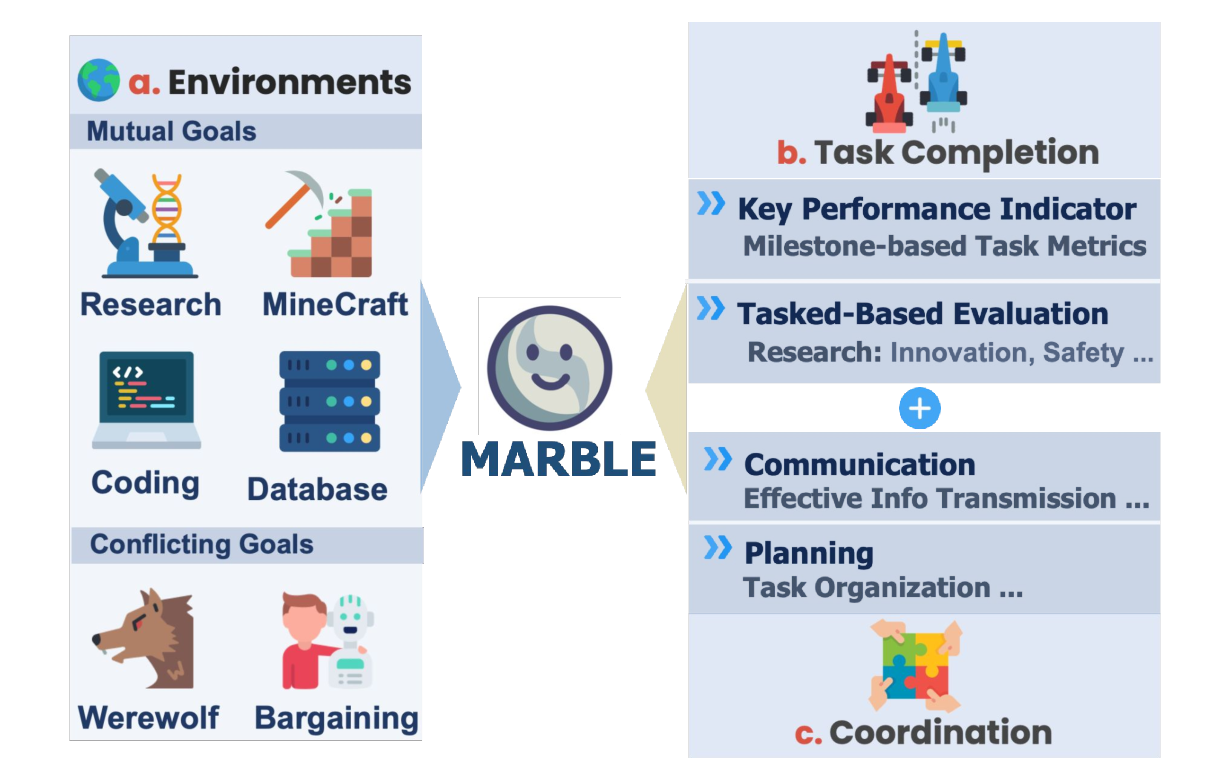
\includegraphics[width=\linewidth]{graphs/Introduction.pdf}
    \caption{\textbf{MultiAgentBench 평가 과정 개요}: 다양한 상호작용 환경에서의 다중 에이전트 시스템 조정을 보여 주며, 과제 성능과 조정에 초점을 둔다.}
    \label{fig:overview}
\end{figure}

%\cheng{Illustration still seems vague here, is it possible to add 1-2 sentences in the figure to explain the scenario or clearly indicates what the metrics measure? (given this figure tasks s much spaces?)}

% However, existing benchmarks and evaluations primarily emphasize single-agent interactions or do not fully capture the dynamics of multi-agent coordination. Approaches like MMLU \citep{Hendrycks2020Measuring} and HumanEval \citep{Chen2021Evaluating} assess language understanding or code generation in isolation. Agent-oriented frameworks such as GAIA \citep{Huang2023LanguageAgents} and AgentBench \citep{Lu2023AgentBench} focus on single-agent performance, while others \citep{Sun2023VisualAgentBench} center on narrow domains. Similarly, prior text-based games \citep{Urbanek2019Learning, Cote2019TextWorld, Hausknecht2020Interactive, Ammanabrolu2020Graph} or multi-modal simulators \citep{Kuttler2020NLE, Fan2022Minedojo, Shi2017WorldOfBits, Toyama2021WebArena, Shen2021iGibson, Srivastava2022Behavior} lack a comprehensive setting tailored to LLM-based multi-agent collaboration.
% \kunlun{Mention Why multiagent, 1.scenarios need multi-persona for simulation only multiagent work 2. benefits comparing to single agents: citing paper like scaling llm , the number increase the performance on coding task, benefits in the efficiency and expand the }

% \kunlun{Specify why original dataset would not elicit the cooperation easily}
% \kunlun{Previous constraints}

% Despite the growing interest, evaluating the effectiveness of LLM-based multi-agent systems remains a significant challenge. Current benchmarks predominantly focus on single-agent settings or evaluate task completion without accounting for multi-agent dynamics. Benchmarks like MMLU \citep{Hendrycks2020Measuring} and HumanEval \citep{Chen2021Evaluating} assess language understanding and code generation in isolation. Frameworks such as GAIA \citep{Huang2023LanguageAgents} and AgentBench \citep{Lu2023AgentBench} focus on single-agent interactions within environments that do not inherently require multi-agent coordination. Other works, like Visual Agent Bench \citep{Sun2023VisualAgentBench}, evaluate agent performance in specific domains but lack a comprehensive assessment of multi-agent collaboration.

% Historically, text-based game environments have been employed for language agent evaluation \citep{Urbanek2019Learning, Cote2019TextWorld, Hausknecht2020Interactive, Ammanabrolu2020Graph}. However, these environments often suffer from limitations such as closed, discrete action spaces and a narrow focus on commonsense grounding. Recent attempts on embodied agents have employed complex multi-modal simulators based on games \citep{Kuttler2020NLE, Fan2022Minedojo}, graphical user interfaces (GUIs) \citep{Shi2017WorldOfBits, Toyama2021WebArena}, and indoor scenes \citep{Shen2021iGibson, Srivastava2022Behavior}. Despite their complexity, these simulators do not accurately reflect the practical use cases of LLMs, and their multi-modal nature creates hurdles for the evaluation of existing text-only LLMs. Furthermore, most current benchmarks focus on single environments and fail to provide a comprehensive overview of LLMs across diverse application scenarios.
% \cheng{logic could be more coherent if written like this: what ability previous benchmarks emphasize? -> What are the unique traits that multi-agent benchmark demands? -> all previous ones fail to capture these traits -> this motivates our design}
% Despite these advances, current evaluation paradigms remain inadequate for multi-agent scenarios. Single-agent benchmarks like \kunlun{agentbench, GAIA}, MMLU \citep{Hendrycks2020Measuring} and HumanEval \citep{Chen2021Evaluating} fail to capture coordination dynamics, while domain-specific frameworks \citep{Sun2023VisualAgentBench} lack cross-task generalizability. Text-based games \citep{Ammanabrolu2020Graph} and multi-modal simulators \citep{Srivastava2022Behavior} either impose restrictive action spaces or require non-textual interfaces incompatible with LLM agent capabilities. Crucially, existing benchmarks overlook three fundamental aspects of multi-agent systems: (1) emergent coordination patterns in open-ended tasks, (2) strategic competition dynamics, and (3) scalability across agent populations \citep{agashe2024llmcoordinationevaluatinganalyzingmultiagent}.
LLM 역량이 크게 발전했음에도 현재의 평가 패러다임은 다중 에이전트 시나리오에 여전히 충분하지 않다. AgentBench~\citep{liu2023agentbench}, VisualAgentBench~\citep{Sun2023VisualAgentBench}, GAIA~\citep{mialon2023gaia}, ToolBench~\citep{qin2024toolllm}, HumanEval \citep{Chen2021Evaluating} 같은 전통적인 단일 에이전트 벤치마크는 주로 고립된 추론과 생성에 초점을 맞추며, 다중 에이전트 상호작용에 내재한 동역학을 간과한다.


% This limitation becomes particularly evident when considering real-world applications. In collaborative coding \citep{huang2023agentcoder, Opendevin2024, SWEGym2024, SyncMind2025}, naively implemented multi-agent systems already achieve ??\% higher success rates \kunlun{how evaluate} than single agents by decomposing tasks through structured communication \citep{islam2024mapcoder}. Similarly, in gaming environments like Minecraft \citep{yu2024minelandsimulatinglargescalemultiagent}, preliminary results show that agent teams demonstrate ?? faster task completion through role specialization. However, current evaluation methods cannot quantify these coordination benefits, leaving critical questions unanswered: How do communication topologies \heng{maybe calling it as communication graph topologies is clearer} affect task performance? What metrics capture the evolution of competition strategies? How do agent coordination strategies and other modules influence coordination efficiency? \cheng{These three questions seems very loosely connected. Could we actually identify a key point in each question to correspond with the key traits you mention above? topology -> the key in investigating emergent coordination pattern, etc. Currently seems too many points are brought up in the introduction part, let's be focused?}


% To address these gaps, we introduce \textbf{MultiAgentBench}, a benchmark that systematically evaluates LLM-based multi-agent systems across task-solving and simulation scenarios. \kunlun{Coordination, Competition}.
% \
% We incorporate new metrics for evaluating both task completion and coordination quality. For task-solving, we define a \textbf{Key Performance Indicator} (KPI) \kunlun{group inner competition} \kunlun{scaling on agents number, or } that reflects milestone-based progress in an agent-based perspective to evaluate the average contributions per agent. For \textbf{coordination}, we quantify planning quality and communication effectiveness through structured Planning and Communication scores~\kunlun{communication quality, wether they communicated}. Competition ~\kunlun{rule-based, tackle competition strategies->remark, competition the same thing as coordination when two groups}. Additionally, we experiment with various coordination protocols (e.g., star, chain, tree, graph) and leverage advanced strategies like Chain of thought~\citep{wei2022chain}, ReACT~\citep{yaoreact}. We further propose a novel cognitive planning approach called \textbf{Cognitive Planning} that significantly improves planning performance.

% \kunlun{to strengthen the coordination, and the competition is the main difference from single agent and where it left to be explored}
% To address this gap, we introduce \textbf{MultiAgentBench}, a comprehensive benchmark designed to evaluate LLM-based multi-agent systems across a range of task-solving and simulation scenarios. Our framework not only measures suitable tasks for multi-agent coordination but also introduces novel and systematic metrics to assess coordination quality.\cheng{summarize the advantages into several key points and  list them clearly: how we are different? - i) multiple domains ii) consider both competition and coordination, iii) new tailored metrics, iv) enables various communication topology v) enables various reasoning methods, vi) enables integration of external module? (choose 3-4 points that you want to emphasize, and make it clear)} \kunlun{more details about how metrics help evaluate the coordination and the competiton here including the planning, communication, KPI: inter competition } Specifically, motivated by human organizations, we define a \textbf{Key Performance Indicator} (KPI) that tracks milestone-based progress and individual agent contributions, as well as structured metrics for planning quality and communication effectiveness\cheng{seems emphasizing KPI here? what about other metrics}. Additionally, we experiment with multiple agent coordination protocols, including star, chain, tree, and graph topologies, evaluating different reasoning strategies for the planning modules like Chain of thought~\citep{wei2022chain}, ReACT~\citep{yaoreact}, and further proposing a group discussion and cognitive planning method.  \heng{the graph topology based communication protocles is very new, emphasize that in abstract too}


이 공백을 해결하기 위해, 우리는 광범위한 과제 해결 및 시뮬레이션 시나리오에서 LLM 기반 다중 에이전트 시스템을 평가하도록 설계된 종합 벤치마크 \textbf{MultiAgentBench}를 제안한다. MultiAgentBench는 몇 가지 핵심 장점을 제공한다. (1) \textit{다중 도메인 평가:} 벤치마크는 협업 코딩부터 게임까지 다양한 도메인을 포괄하여 넓은 실제 적용 가능성을 보장한다. (2) \textit{조정과 경쟁 포착:} 전통적인 단일 에이전트 벤치마크와 달리 MultiAgentBench는 조정 동역학과 경쟁적 상호작용을 명시적으로 측정하여, 다중 에이전트 환경의 고유한 어려움을 드러낸다. (3) \textit{맞춤형 지표와 유연한 프로토콜:} 우리는 milestone 진행과 개별 기여를 추적하는 \textit{Key Performance Indicator (KPI)}를 포함한 새로운 지표를 제안하여 계획 품질과 의사소통 효과를 체계적으로 평가한다. 또한 우리의 프레임워크 \textbf{MARBLE}(\textbf{M}ulti-agent coo\textbf{R}dination \textbf{B}ackbone with \textbf{L}LM \textbf{E}ngine)은 star, chain, tree, 혁신적인 graph 기반 접근 등 다양한 communication topology를 지원하고 여러 추론 전략을 수용한다.

% \kunlun{Our exp shows that...}

% Our contributions can be summarized as follows:
% (1) We develop \textbf{MultiAgentBench}, a benchmark that rigorously evaluates LLM-based multi-agent systems in diverse interactive environments, capturing both collaborative and competitive dynamics.
% (2) We propose novel evaluation metrics that measure the success of multi-agent coordination, including milestone-based KPIs and structured planning and communication scores, and introduce comprehensive evaluation methods for evaluating the coordination and competition of multi-agent LLMs.
% \kunlun{Claiming we also found the aha-moment for the multiagent coordination that they actually learn how to collaborate with emergent social  behaviors and navigate the hope for AGI(citing the AGI paper)}

% \kunlun{2. marble frame work}
% \kunlun{3. innovative metrics for both task and coordination evaluation}
% \kunlun{Introducing the competition evaluation and the competition score, introducing more experiment results and the emergent behaviors part}
% \kunlun{We consider competition in three parts: conflicting goals task, its task results showcase its competition ability; 2. KPI score is the inner competition metrics, 3. designing the prompt for planning and communication including its competitive aspects}

우리의 기여는 다음과 같이 요약할 수 있다.
(1) 우리는 \textbf{MultiAgentBench}와 \textbf{MARBLE} 프레임워크를 도입한다. 이는 여섯 가지 다양한 상호작용 시나리오에서 LLM 기반 다중 에이전트 시스템을 엄밀하게 평가하고 협업 및 경쟁 동역학을 모두 포착하는 종합 벤치마크이다. 특히 cognitive planning 기능은 milestone 달성률을 3\% 향상시킨다.
(2) 우리는 과제 성공뿐 아니라 조정 품질도 평가하는 혁신적 평가 지표를 제안한다. 이 지표에는 milestone 기반 KPI, 구조화된 planning 및 communication score, 그리고 상충 목표 과제, 내부 성능 지표, 계획과 의사소통의 경쟁적 측면을 포착하는 전용 competition score가 포함된다.
(3) 우리의 실험은 다중 에이전트 조정에서 몇 가지 ``aha-moments''를 드러낸다. 에이전트는 창발적 사회 행동을 보이기 시작하며, AGI 수준 협업을 향한 유망한 통찰을 제공한다~\citep{feng2024how}.
% \kunlun{can omit here if the article is too long}


% To address these challenges, we introduce \textbf{MultiAgentBench}, a multi-dimensional benchmark designed to evaluate LLM-based multi-agent systems across a spectrum of different environments and tasks. MultiAgentBench encompasses both task-solving and simulation scenarios.


% In addition to introducing MultiAgentBench, we propose methods to enhance the coordination abilities of LLM-based agents. We leverage multi-head Tree-of-Thought strategies \citep{Yao2023TreeofThought} to allow agents to explore multiple reasoning paths simultaneously, facilitating better decision-making and planning. Furthermore, we employ Low-Rank Adaptation (LoRA) tuning techniques \citep{Hu2021LoRA} to efficiently fine-tune LLMs for multi-agent coordination tasks without extensive retraining.
% \todo{add more about the coordination study}
% \todo{add more results of our metric design}

% Our contributions can be summarized as follows:

% \begin{itemize} \item We design new metrics to better evaluate coordination, planning among agents.\zhenhailong{maybe add the name/abbreviation and highlight of the metric, e.g., KPI?}

% \item We develop \textbf{MultiAgentBench}, a comprehensive benchmark focusing on evaluating multi-agent coordination. \item We introduce a novel methods called Cognitive Planning to enhance the planning and coordination capabilities of LLM-based agents. \end{itemize}

% \begin{figure*}[h]
%     \centering
%     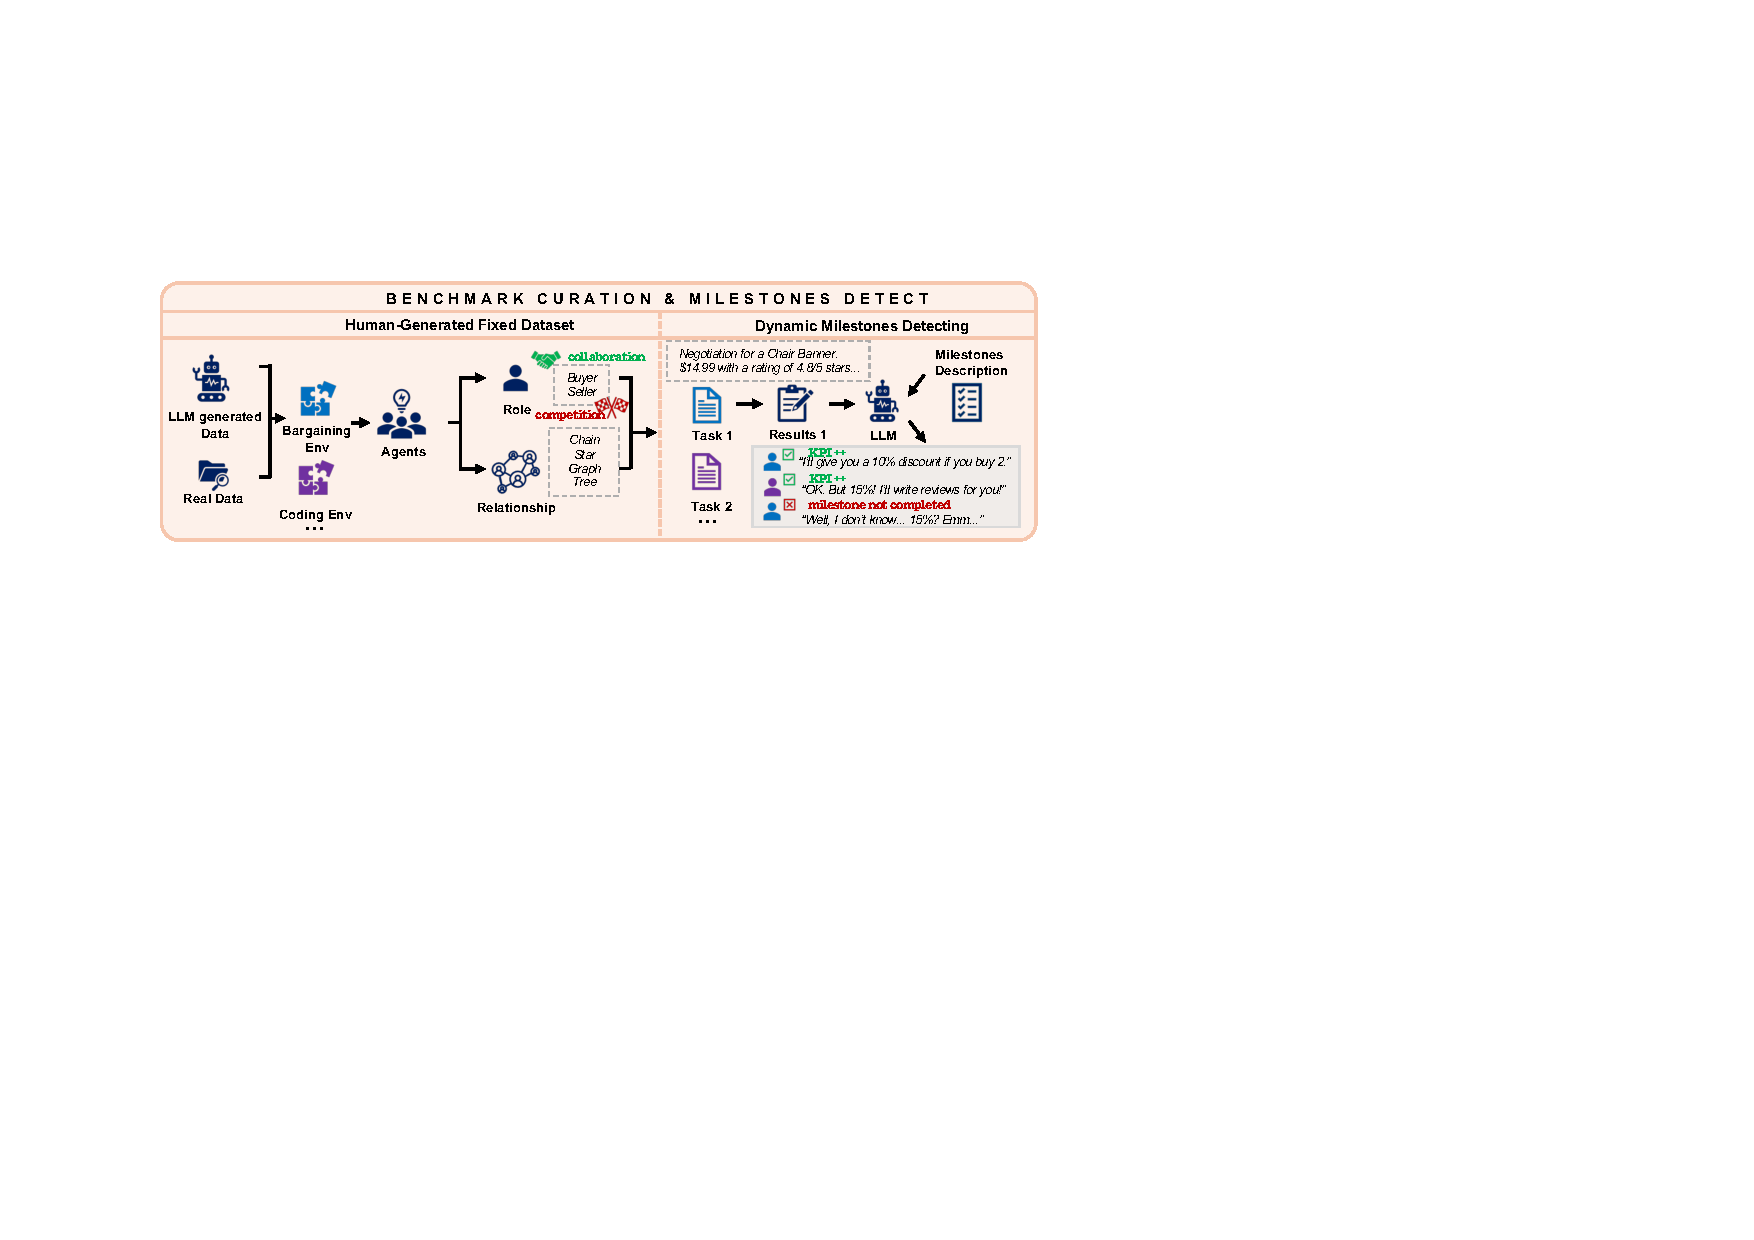
\includegraphics[width=\linewidth]{graphs/marble_graph.pdf}
%     \caption{Overview of the methodology: illustrating the milestones generation process, evaluation inputs for iterations, and metrics for task completion and coordination. Key components include task-based evaluation, KPI tracking, and collaboration between agents through planning, action, and communication.}
%     \label{fig:method}
% \end{figure*}

\begin{figure*}[htbp]
    \centering
    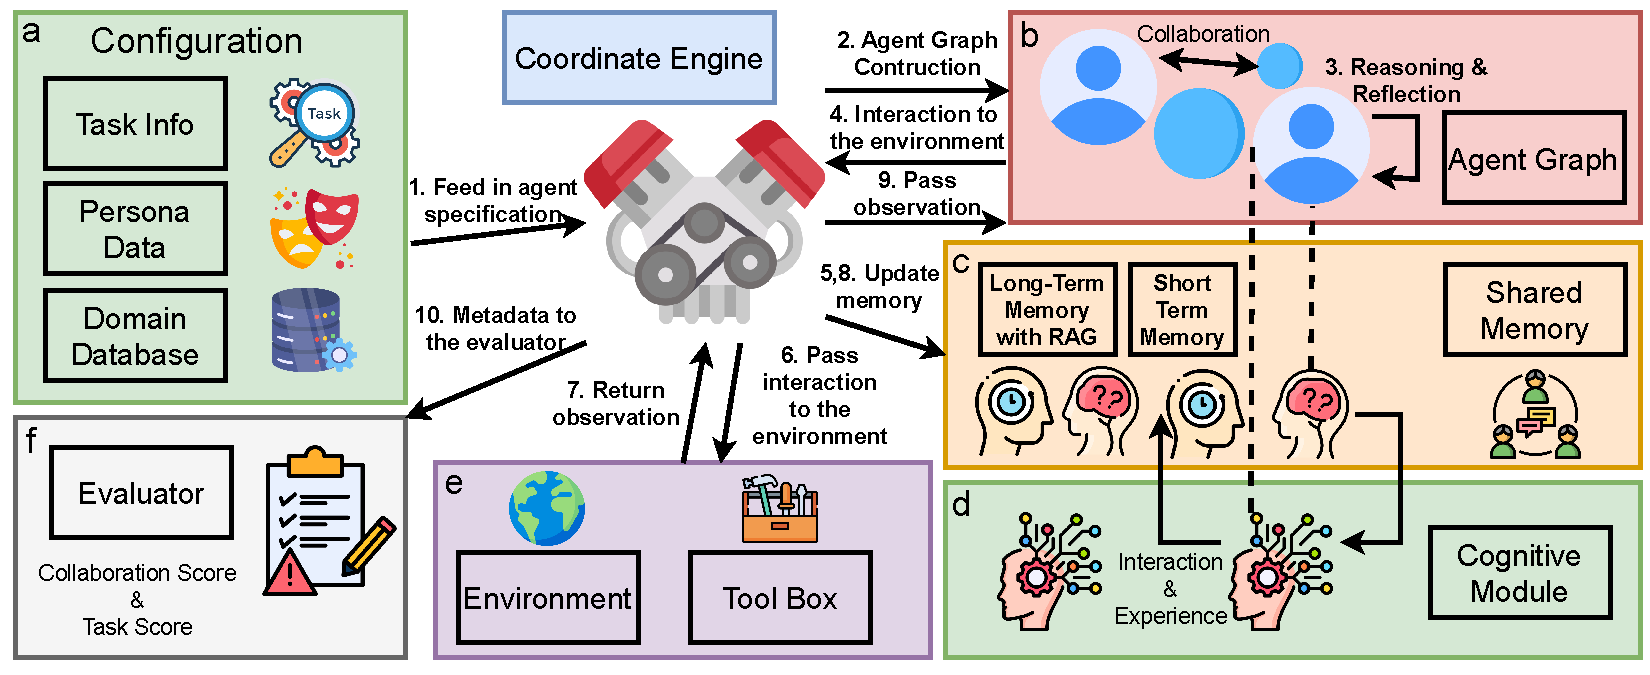
\includegraphics[width=\linewidth]{graphs/engine.pdf}
    \caption{MARBLE \icon: coordination engine과 cognitive module을 통해 과제 정보, persona data, domain database, memory module, 환경 사이의 상호작용을 보여 준다.}
    \label{fig:engine}
\end{figure*}

\section{관련 연구}
% Existing works on LLM-driven multi-agent systems, such as AgentBench~\citep{liu2024agentbench} and VisualAgentBench~\citep{liu2024visualagentbenchlargemultimodalmodels}, primarily focus on single-agent tasks. Recent studies have explored agent collaboration in various domains like scientific problem solving~\citep{tang2024prioritizing, chan2024mlebenchevaluatingmachinelearning}, coding~\citep{jimenez2024swebench}, and gaming~\citep{wang2023voyageropenendedembodiedagent}. However, a holistic evaluation framework that comprehensively analyzes coordination, role differentiation, and emergent agent behavior is still missing.

% We compare our framework with existing benchmarks and focus on expanding the evaluation to multi-agent settings, emphasizing the importance of planning, communication, and shared and individual memory capabilities in agent systems.

\subsection{LLM 기반 다중 에이전트 시스템}

LLM 기반 다중 에이전트 시스템은 여러 도메인에서 협업적 문제 해결을 가능하게 했다~\citep{Park2023GenerativeAgents, li2023camelcommunicativeagentsmind, chen2023agentversefacilitatingmultiagentcollaboration}. 이러한 시스템은 문헌 검토와 실험 설계를 통해 과학 연구를 지원하고 \citep{zhou2024hypothesis, agarwal2024litllmtoolkitscientificliterature}, 코드 생성과 유지보수 \citep{bouzenia2024repairagent}를 포함한 소프트웨어 공학 과제 \citep{huang2023agentcoder, wu2023autogen, zhou2023agents, hong2024metagpt, ishibashi2024self, islam2024mapcoder, openhands, zhugegptswarm}, 게임 응용 \citep{chen2023gamegpt}에도 활용된다. Minecraft에서는 에이전트가 건설부터 내비게이션까지 복잡한 과제를 수행한다 \citep{wang2023voyageropenendedembodiedagent, chen2023agentversefacilitatingmultiagentcollaboration, yu2024minelandsimulatinglargescalemultiagent, dong2024villageragentgraphbasedmultiagentframework}.

% In gaming, LLM-powered agents simulate human-like behavior and contribute to creating more realistic environments. For example, GameNGen, the first neural-driven game engine, enables real-time interaction in complex environments, simulating games like DOOM at over 20 frames per second on a single TPU \cite{valeveski2024diffusion}. Similarly, MindAgent introduces CUISINEWORLD, a novel gaming scenario and benchmark for evaluating multi-agent collaboration efficiency, enabling agents to collaboratively play games and solve tasks \cite{gong2023mindagent}.

% In world simulation scenarios, these multi-agent systems excel in tasks that require judgment, self-awareness, and strategic decision-making. For example, multi-agent LLM systems have been applied to games like \textit{Chameleon} and \textit{Undercover}, where they demonstrate abilities in social deduction and deception, as well as in game theory scenarios like \textit{Cost Sharing} and \textit{Public Goods}, which highlight their capacity for strategic collaboration and resource management. \citep{xu2023magic}
% Additionally, these systems are applied in healthcare for more accurate diagnostics and decision making\citep{ke2024enhancing, kim2024adaptive}. In the business world, multi-agent LLM systems optimize tasks such as customer support, sales, and operational workflows \citep{chen2024agentverse}. Moreover, in education, multi-agent systems are used for personalized tutoring and collaborative learning \citep{gosling2024multi}. LLM-based multi-agent systems are also utilized in urban planning, logistics, and resource management, enhancing decision-making through simulations and coordination \citep{zhou2024largelanguagemodelparticipatory}. Despite these successes, challenges remain, including ensuring effective communication among agents, handling emergent behaviors, and scaling these systems for real-world applications \citep{agashe2024llmcoordinationevaluatinganalyzingmultiagent}. These issues highlight the need for robust frameworks to assess and improve multi-agent coordination, which our work aims to address.
GameNGen은 DOOM에서 실시간 상호작용을 가능하게 하고 \citep{valeveski2024diffusion}, CUISINEWORLD는 다중 에이전트 협업을 벤치마크한다 \citep{gong2023mindagent}. 응용 범위는 사회적 추론 게임, game theory \citep{xu2023magic}, healthcare \citep{ke2024enhancing, kim2024adaptive}, business \citep{chen2024agentverse}, education \citep{gosling2024multi}, urban planning \citep{zhou2024largelanguagemodelparticipatory}까지 확장된다. 진전에도 불구하고 communication, emergent behavior, scalability에는 여전히 문제가 남아 있으며 \citep{agashe2024llmcoordinationevaluatinganalyzingmultiagent}, 이는 강건한 평가 프레임워크의 필요성을 뒷받침한다.

% \kunlun{More Comparison between the existing benchmarks make a table}
% \kunlun{adding more work like waragent,}

\subsection{다중 에이전트 협업}

% The success of single LLM-based agents in reasoning and planning has inspired collaborative frameworks involving multiple LLM agents, enabling the integration of specialized capabilities and often surpassing the performance of individual models \citep{zhang2023exploring}. Communication topologies explored for multi-agent collaboration include non-interactive setups where agents operate independently, chain structures where outputs are passed sequentially, star configurations with a central agent directing others, hierarchical tree arrangements with parent-child relationships, and complex graph-based systems facilitating dynamic interactions \citep{zhou2024hypothesis}. Recent studies have introduced dynamic communication strategies, enabling adaptive collaboration tailored to specific tasks. For instance, frameworks like G-Designer leverage graph neural networks to optimize multi-agent communication and coordination \citep{zhang2024gdesignerarchitectingmultiagentcommunication}. Despite these advances, evaluating aspects like coordination, role differentiation, and emergent behaviors in LLM-based systems remains challenging, emphasizing the need for a comprehensive evaluation framework, which our work seeks to address.

최근 다중 에이전트 시스템의 발전은 두 가지 상호보완적 scaling paradigm을 강조한다. 하나는 에이전트의 추론과 적응성을 강화하는 \textit{cognitive scaling}이고, 다른 하나는 대규모 에이전트 집단을 활용해 창발 행동을 이끌어내는 \textit{population scaling}이다 \citep{zhugegptswarm, qian2024scalinglargelanguagemodelbasedmultiagentcollaboration}.

Cognitive scaling은 dynamic architecture adaptation과 self-organizing coordination strategy 같은 메커니즘을 탐구하여 에이전트 의사소통의 가장 효과적인 패턴을 찾는다 \citep{zhugegptswarm}. 한편 population-based scaling은 에이전트 수가 증가하면서 hierarchy delegation, decentralized consensus 등 다양한 협업 패턴을 통해 집단적으로 상호작용할 때 비선형적 성능 향상을 보인다 \citep{qian2024scalinglargelanguagemodelbasedmultiagentcollaboration}.
이러한 접근은 지정학적 갈등 시뮬레이션 \citep{hua2024warpeacewaragentlarge}부터 과학적 발견 workflow \citep{zhou2024hypothesis, zhang2025crewfacilitatinghumanaiteaming}까지 복잡한 응용을 가능하게 한다.

% Recent advances in multi-agent systems reveal two complementary scaling paradigms: \textit{cognitive scaling} through dynamic architecture optimization \citep{zhugegptswarm} and \textit{population scaling} via agent orchestration \citep{qian2024scalinglargelanguagemodelbasedmultiagentcollaboration}. Cognitive approaches treat agents as optimizable computational graphs, achieving improved performance through automated topology pruning \citep{zhugegptswarm}, while population-based methods demonstrate logistic performance growth with agent count through irregular collaboration patterns \citep{qian2024scalinglargelanguagemodelbasedmultiagentcollaboration}. \heng{not sure what you mean by 'irregular collaboration patterns'. elaborate and illustrate?} \heng{'agent count through irregular collaboration patterns' very hard to parse} These paradigms enable complex applications ranging from geopolitical conflict simulation \citep{hua2024warpeacewaragentlarge} to scientific discovery workflows \citep{zhou2024hypothesis}.

% \kunlun{change the cognitive statement into something else, scaling in numbers, coordination strategies, emergent behaviors analysis, social, no taxonomy needed}

% Architectural innovations address core coordination challenges: Graph neural networks optimize communication efficiency \citep{zhang2024gdesignerarchitectingmultiagentcommunication}, while hierarchical structures enhance task decomposition \citep{zhou2024hypothesis}. Our benchmark extends these foundations through two axes: 1) \textit{Topology Robustness} testing across communication graphs, 2) \textit{Emergent Strategy Analysis} quantifying competitive adaptation. This framework reveals that automated topology optimization reduces coordination overhead by ??\% compared to fixed architectures \citep{zhugegptswarm}, while irregular collaboration patterns outperform regular structures in large-scale coordination \citep{qian2024scalinglargelanguagemodelbasedmultiagentcollaboration}.
% \kunlun{todo:make sure the data and content cited is accurate}


% \section{System Architecture and Design}
% The proposed multi-agent system architecture includes the following components:

% \subsection{Coordination and Task Completion}
% Figure~???????????????????????????????????????????????????????????????????????????????????????????????????????????????????????????????????????????????????????????????????????????????????????????????????????????????????????????????????????????????????????????????????????????\ref{fig:results} provides insights into the performance of agents across different task scenarios, and we find significant trade-offs between planning efficiency and task completion success.



% \begin{itemize}
%     \item \textbf{Coordination Engine}: Manages agent behavior, interactions, and constructs the agent graph for collaboration. Different collaboration strategies, such as group chatting and hierarchical planning, are implemented.
%     \item \textbf{Agent Graph}: Represents relationships among agents, enabling reasoning, reflection, and adaptive collaboration.
%     \item \textbf{Shared and Individual Memory}: Allows agents to retain both collective and individual knowledge, facilitating coordinated decision-making.
%     \item \textbf{Cognitive Module}: Supports adaptive behavior and evolving strategies with accumulated experience.
%     \item \textbf{Interactive Environment and Tool Box}: Provides agents with tools to interact with the environment and complete assigned tasks.
%     \item \textbf{Evaluator}: Measures agent performance across various dimensions, providing feedback to improve collaboration.
% \end{itemize}

% The information flow in our system starts with the coordination engine, which constructs an agent graph based on task data. The agents interact with the environment through the provided tools, while shared memory aids in collaboration. Figure~??????????????????????????????????????????????????????????????????????????????????????????????????????\ref{fig:progress} illustrates the architecture.




% \subsection*{Methodology}

% \begin{figure*}[t]
%     \centering
%     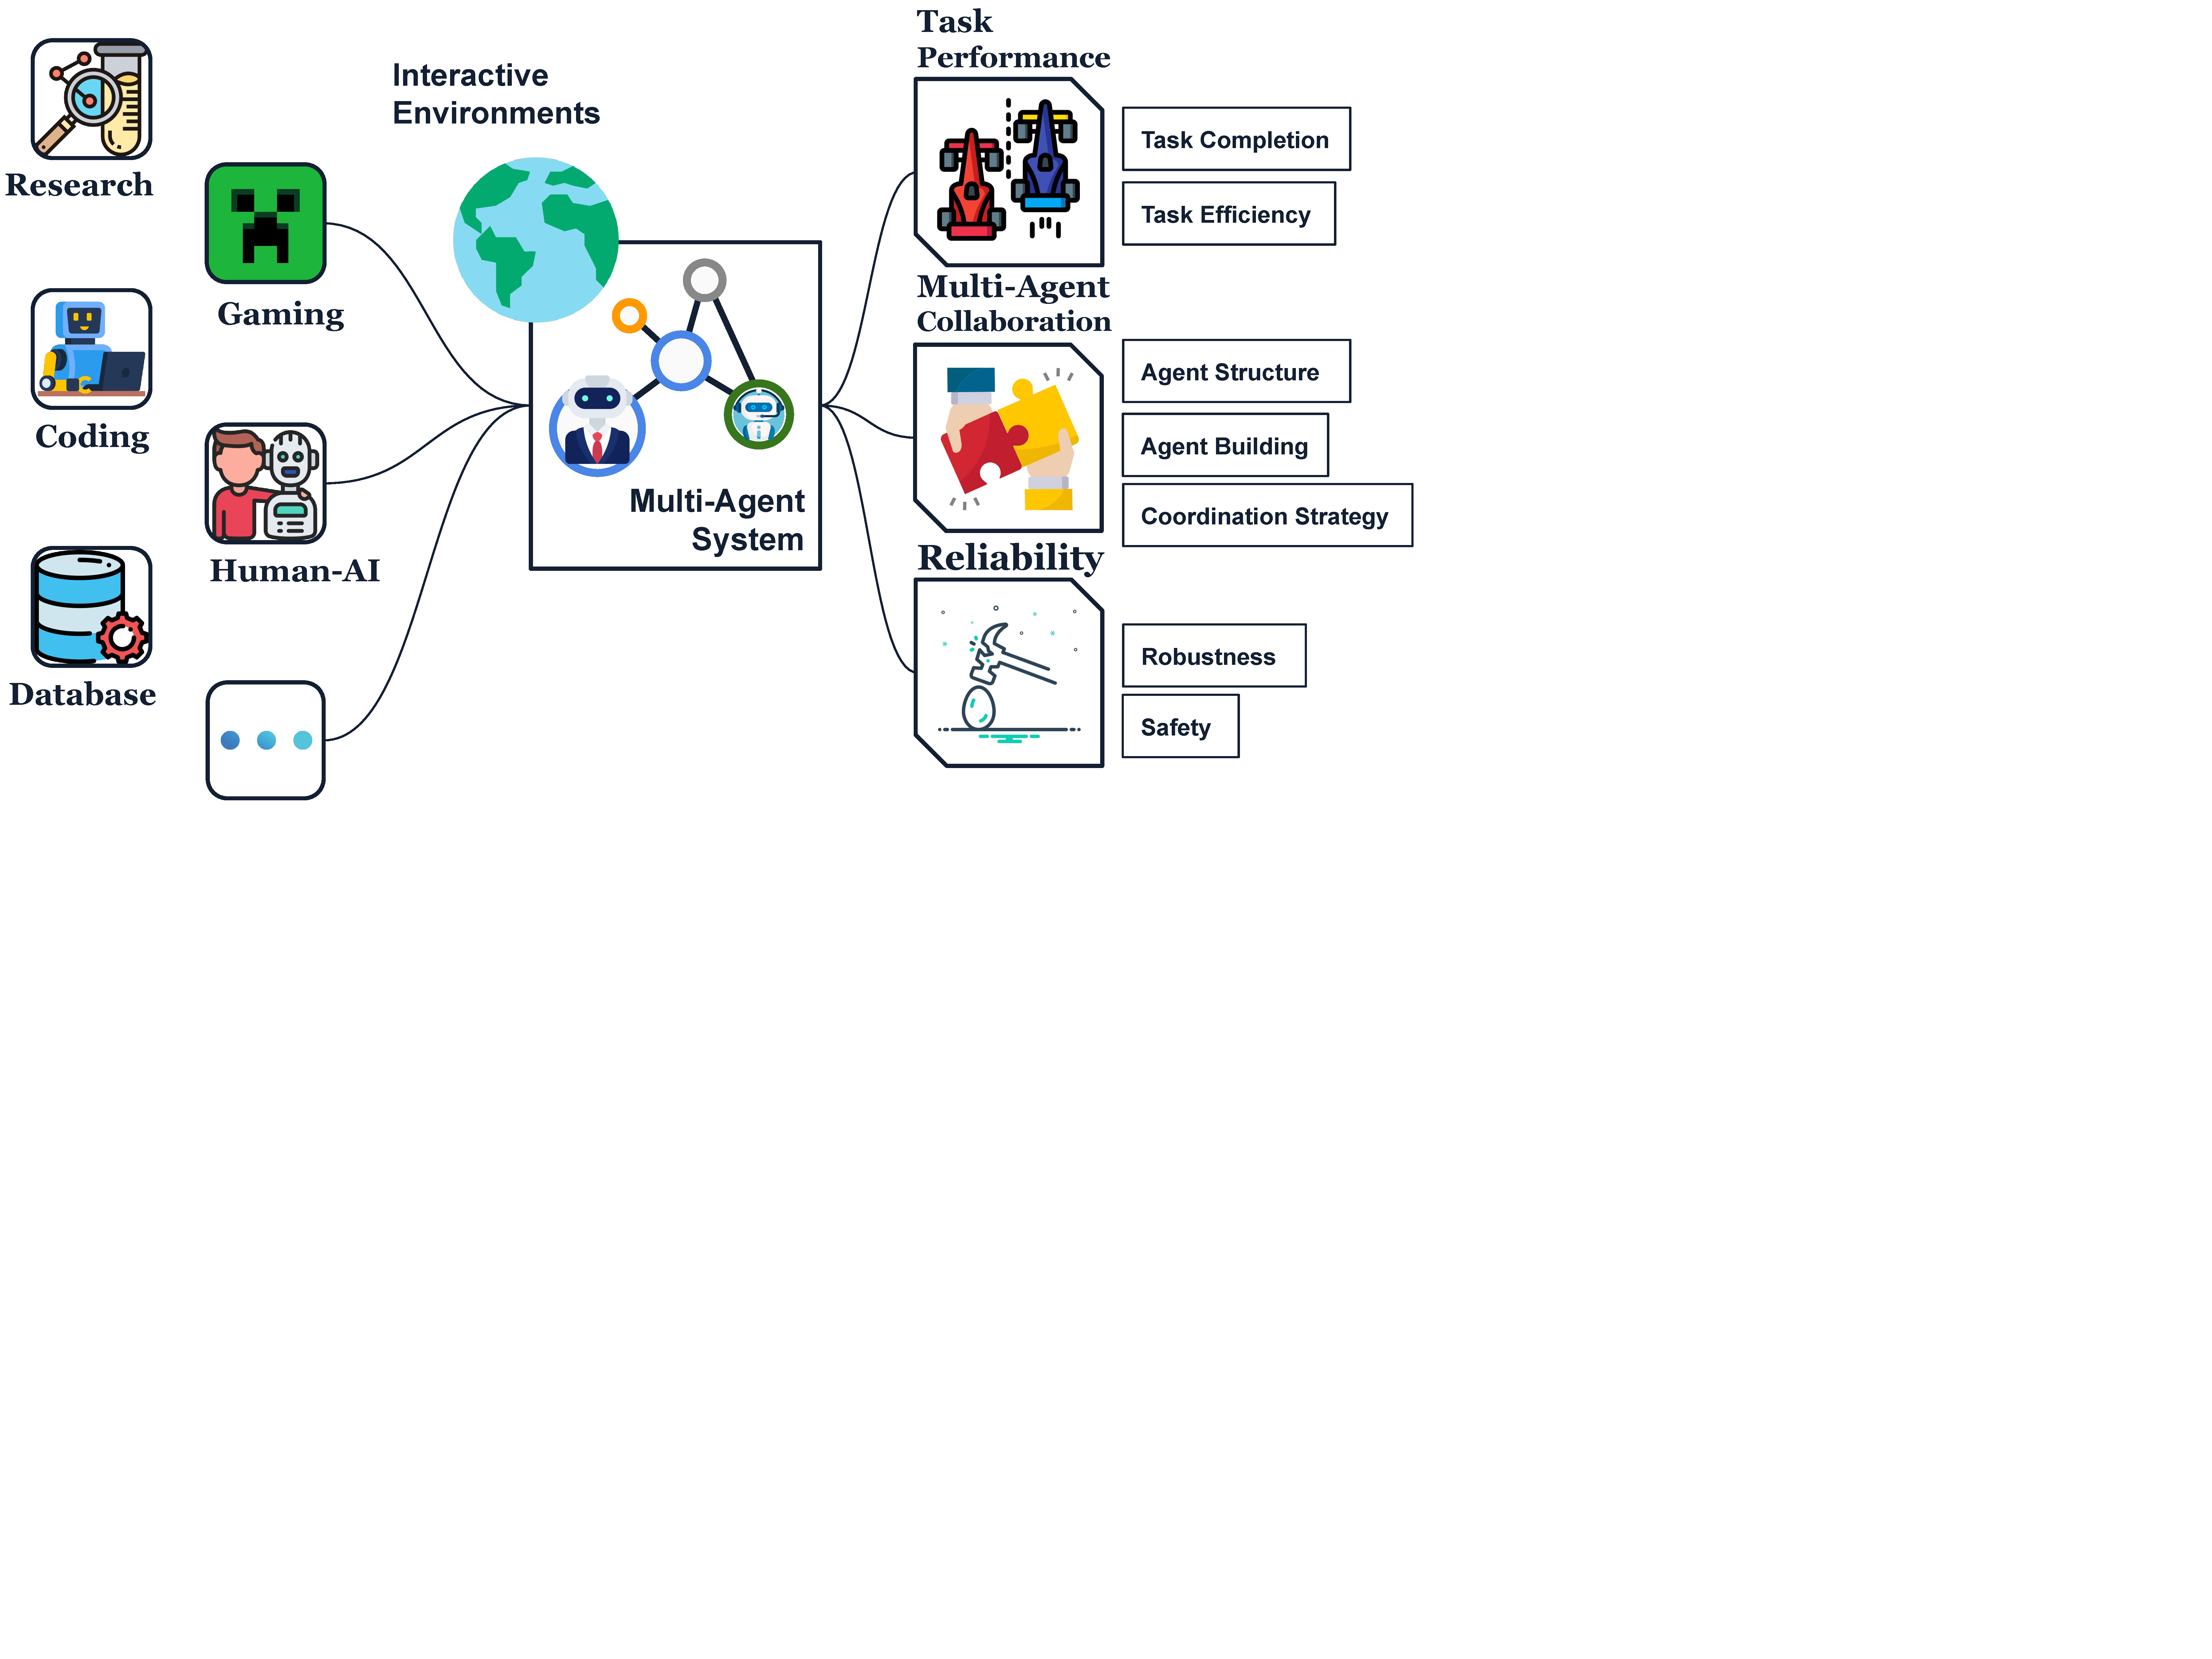
\includegraphics[width=0.96\linewidth]{graphs/Illustration.pdf}
%     \caption{The Main Multi-agent Eval Pipeline}
%     \label{fig:progress}
% \end{figure*}


% We designed a series of interactive environments for evaluating the multi-agent system. Each environment provides unique challenges, allowing us to assess aspects of task performance, collaboration, and reliability.

% The evaluation of the multi-agent system will be conducted through three major dimensions:

% \begin{itemize}
%     \item \textbf{Task Performance}: This dimension will focus on evaluating how effectively the agents complete assigned tasks. It will include metrics such as task completion and efficiency, providing insight into how well the agents achieve their objectives.
%     \item \textbf{Multi-Agent Collaboration}: In this dimension, we will assess the quality of collaboration among agents. We will evaluate aspects such as coordination strategies and workflow building to solve complex problems effectively.
%     \item \textbf{Reliability}: Reliability will be measured by analyzing the robustness and safety of the multi-agent system, ensuring stability under various conditions.
% \end{itemize}

% The system architecture consists of several interlinked modules:

% \begin{itemize}
%     \item \textbf{Coordinate Engine}: The coordinate engine orchestrates agent behavior by managing interactions and constructing the agent graph. The coordinate engine will include different collaboration strategy such as group chatting, hierarchical traverse planning, etc.
%     \item \textbf{Agent Graph}: The agent graph represents relationships among agents, enabling reasoning, reflection, and collaboration.
%     \item \textbf{Shared and Individual Memory}: Agents share a common memory for collective knowledge and maintain individual memory for personalized learning.
%     \item \textbf{Cognitive Module}: The cognitive module supports adaptive behavior, allowing agents to evolve with experience.
%     \item \textbf{Environment and Tool Box}: Agents operate within an interactive environment, using tools provided by the tool box to complete tasks.
%     \item \textbf{Evaluator}: The evaluator analyzes performance and provides feedback for improvement.
% \end{itemize}

% The flow of information starts with the coordinate engine constructing the agent graph based on task data. Agents interact with the environment using various tools, with shared memory facilitating collaboration.

% \textbf{Environment Module }: \zhaochen{todo below in the methodology part}

% \textbf{Memory Module} \xiaocheng{todo below in the methodology part}

% \textbf{Reasoning module}: \zhewang{todo below in the methodology part}

% \textbf{Milestone Generation Part}: \hongyi{To do in the benchmark part}


\section{방법론}
\subsection{프레임워크 설계}

% The proposed framework, illustrated in Figure~\ref{fig:engine}, facilitates multi-agent coordination through interconnected modules that \textbf{support adaptive collaboration}, effective communication, and strategic task execution. Central to this framework is the \textbf{Coordination Engine}, which orchestrates the following primary modules: \textbf{Agent Graph}, and \textbf{Cognitive Module}, more details about different modules can be found on Appendix \ref{framework}. \kunlun{specifying more modules shown on Appendix A.1, citing the graphics}


% \paragraph{Agent Graph Module}
% Transforms configuration data into a graph $G = (V, E)$, where each node $v_i \in V$ represents agent $A_i$, and edges $e_{ij} \in E$ denote relationships like collaboration $(A_i \leftrightarrow A_j)$, supervision $(A_i \rightarrow A_j)$, or negotiation $(A_i \leftrightsquigarrow A_j)$. This graph informs the coordination protocol and underpins collective reasoning and decision-making.

% \kunlun{specify the need and the design of Agent graph}



% \paragraph{Cognitive Module and Communication Module }
% \kunlun{social, relationship aware and memory design}
% Handles internal reasoning and strategic decision-making by integrating shared and individual memories, environment observations, and agent relationships from the graph. Inspired by theory-of-mind, it allows agents to infer others’ intentions and roles, promoting socially intelligent behavior. This module manages prompt construction for reasoning, reflection, and summarization, refining understanding of social structures and communication patterns to adapt strategies over time.
% \kunlun{strength how these modules enable the coordination and competition}

% Two agents $A_i, A_j$ can communicate with each other if $(v_i, v_j) \in G$. Agents are presented the option of communicating with another agent with the communication option provided as a tool. They are also given profiles of the agents they can communicate to, so they can choose which agent to talk to. Then two agents will have a conversation between them until they decide to terminate or the communication exceeds allowed rounds. Finally, the conversation will be summarized and inserted into the Memory of the two agents.
% \paragraph{Coordination Engine & Action Modeule}
% \kunlun{adding function calling style of tool calling citing tool work for actions}
% Guides the execution flow by initializing agents, tasks, and relationships via the Configuration Module, constructing the agent graph with the Agent Graph Module, and preparing the environment and its tool functionalities. Agents then interact with the environment through cognitive processing and memory retrieval, with observations and results updating both memory and cognitive states. The engine iteratively refines agent states and strategies, ensuring continuous learning and enhancement of coordination and task execution efficacy. Upon reaching task-specific milestones or termination conditions, the final results are returned to the evaluator, which provides performance feedback and updates key performance indicators.

% \kunlun{also writing the paragraph how the agents running and coordination within our framework from the relationship to the results how we save then evaluate them. Predefined agents and flixible executing structures: how the whole thing executed}

우리가 제안하는 평가 프레임워크 MARBLE~(Figure~\ref{fig:engine} 참조)은 adaptive collaboration, efficient communication, strategic task execution을 가능하게 하는 상호연결 모듈을 활용하여 강건한 다중 에이전트 조정 시스템을 구축한다. 그 핵심에는 시스템 전반의 매끄러운 상호작용을 보장하기 위해 \textit{Agent Graph}, \textit{Cognitive Module}, \textit{Coordinate Engine}을 포함한 주요 모듈을 초기화하고 동기화하는 \textit{Coordination Engine}이 있다. 추가 모듈의 자세한 설명은 Appendix~\ref{framework}에서 확인할 수 있다.

% \paragraph{Agent Graph Module}
% This module transforms configuration data into a structured graph $G = (V, E)$, where each node $v_i \in V$ represents an agent $a_i$, and each edge $e_{ij} \in E$ encodes various inter-agent relationships such as collaboration $(a_i \leftrightarrow a_j)$, supervision $(a_i \rightarrow a_j)$, or negotiation $(a_i \leftrightsquigarrow a_j)$. \kunlun{refine the math annotation}The design of the Agent Graph is pivotal for capturing dynamic interaction patterns and ensuring scalable coordination across agents. \kunlun{using the agent1 rel agent2 to form the graph, when communicate only communicate with someone with relationship which like in the real-world}

\paragraph{Agent Graph Module}
이 모듈은 configuration data를 구조화된 그래프 \(G = (\mathcal{A}, E)\)로 변환한다. 여기서 \(\mathcal{A} = \{a_1, a_2, \dots, a_n\}\)는 에이전트 집합을 나타내며, \(E\)의 각 edge는 \(r \in \mathcal{R}\)이 에이전트 \(a_i\)와 \(a_j\) 사이의 관계를 나타내는 triple \((a_i, r, a_j)\)로 정의된다. 예를 들어 협업 관계는 \((a_i, \texttt{collaborates}, a_j)\), 감독은 \((a_i, \texttt{supervises}, a_j)\), 협상은 \((a_i, \texttt{negotiates}, a_j)\)로 표기한다. 이러한 triple 관계를 기반으로 그래프를 구성함으로써, 이후의 의사소통과 조정이 명시적으로 정의된 관계를 가진 에이전트 사이에서만 일어나도록 하며, 이는 실제 세계의 상호작용 패턴을 반영한다.


% \paragraph{Cognitive Module}
% The Cognitive Module underpins internal reasoning by integrating shared and individual memories, real-time environmental observations, and relational data from the Agent Graph. Inspired by cognitive theories of self-reflection and theory-of-mind \citep[e.g.,][]{premack1978}, this module generates expected outcomes and progress for each task and stores them in memory. In subsequent iterations, actual performance is compared against these expectations to produce evolving experiences. These experiences guide adjustments in planning, enabling agents to continuously refine their strategies and adapt to unexpected outcomes. \kunlun{cognitive module in responsible agent evolving, and social intelligence important for the multiagent coordination, with agent self involving persona, agent relationship, its intter action reasoning method(cot, react, ..) updating its memory, social aware etc}

\paragraph{Cognitive Module}
Cognitive Module은 다중 에이전트 조정에서 책임 있는 에이전트 진화와 사회적 지능의 중심이다. 이 모듈은 각 에이전트의 persona, 에이전트 간 관계, Chain-of-Thought~\citep{wei2023chainofthoughtpromptingelicitsreasoning} 및 ReACT~\citep{yao2023reactsynergizingreasoningacting} 같은 추론 전략을 포함하는 포괄적 내부 상태를 유지하고 갱신한다. 핵심적으로 이 접근은 인간이 사회적 단서, 과거 경험, 맥락 정보를 바탕으로 정신 모델을 지속적으로 갱신하는 방식과 유사하게, theory-of-mind와 social intelligence의 요소를 결합하여 인간의 인지 과정을 모사한다 \citep[e.g.,][]{premack1978}. 인지적, 사회적, 적응적 메커니즘의 결합은 우리 시스템의 중추를 형성하며, 에이전트가 복잡한 환경에서 전략을 동적으로 조정하고 협업적으로 진화할 수 있게 한다.


\begin{figure*}[ht]
    \centering
    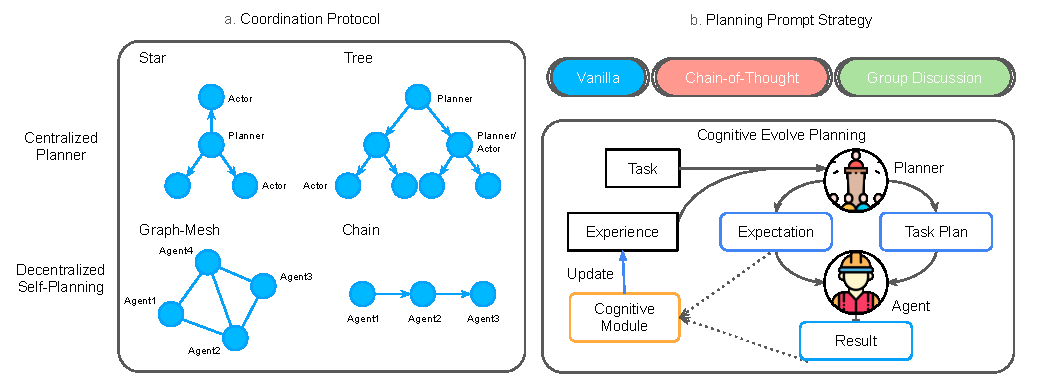
\includegraphics[width=\textwidth]{graphs/coordination.pdf}
    \caption{\textbf{조정 프로토콜과 planning prompt 전략의 예시}.
    \textbf{(a)}는 star, tree, graph, chain 같은 centralized 및 decentralized planning 구조를 보여 준다.
    \textbf{(b)}는 효과적 planning을 위해 iterative feedback과 task update를 통합하는 group discussion 및 cognitive prompt 같은 전략을 설명한다.}
    \label{fig:coordination}
\end{figure*}

% \subsubsection{Coordination Engine}
% The Coordination Engine orchestrates the overall execution flow of the system. It initializes agents, tasks, and inter-agent relationships via a dedicated Configuration Module and constructs the Agent Graph to represent these dynamics.

% \kunlun{define what is a planner within the coordination engine and what is an actor, a planner plans the task input for the actor, actor is the agent within the Agent Graph and can use tools interact with the env or other agents}

% \kunlun{define 4 coordination protocol clear below}


%  Our approach considers four Coordination protocol---\textbf{star}, \textbf{tree}, \textbf{graph}, and \textbf{chain}. Specifically, \textbf{star} and \textbf{tree} are centralized methods where one (or a hierarchy of) planner(s) manages task allocation and aggregates feedback, while \textbf{graph} and \textbf{chain} rely on decentralized coordination through peer-to-peer interactions and sequential task handoffs.

% \paragraph{Centralized Coordination: Star \& Tree.}
% In the \textbf{star} configuration, a single central planner assigns tasks to all agents and consolidates their feedback, making it effective for tasks that require strong oversight but potentially limited in scalability. The \textbf{tree} structure builds on this by organizing agents hierarchically: a top-level planner delegates tasks to subordinate planners, combining centralized control with enhanced scalability for complex tasks.

% \paragraph{Decentralized Coordination: Graph \& Chain.}
% The \textbf{graph} configuration utilizes a network of interconnected agents that communicate directly, enabling concurrent planning and distributed decision-making. In contrast, the \textbf{chain} structure arranges agents sequentially, where each agent passes decisions to the next. This approach is well-suited for tasks with sequential dependencies, though it may constrain parallel processing.

% \paragraph{Planner Design and Enhancements.}
% \kunlun{updating the new method of cognitive evolving with expectation result and experience update for better task  planning }
% \kunlun{for the star coordination style, ablation on different planning stratigies}
% Building on these structures, our approach employs iterative, feedback-driven planning. A zero-shot chain-of-thought prompt equips the planner with the target task, agent profiles, \heng{not sure what agent profile contains, define and give example} and a summary of past subtasks, enabling step-by-step reasoning. The REACT-style mechanism interleaves planning with action, while \textbf{group discussions} allow agents to share insights and constraints. \textbf{Cognitive planning} principles further ensure effective workload distribution and task alignment. Each round concludes with a concise summary of lessons learned, continuously refining the system's coordination and performance.  \kunlun{For cognitive evolve, when generating a task, the expected result and progress are produced and stored in memory; in subsequent iterations, the actual progress is compared with the expectations to generate evolving experiences that inform adjustments to planning if the outcomes fall short, with these experiences continually saved and updated to guide future plans.}

\subsubsection{Coordination Engine}
Coordination Engine은 시스템의 전체 실행 흐름을 조율한다. 전용 Configuration Module을 통해 에이전트, 과제, 에이전트 간 관계를 초기화하고, 이러한 동역학을 표현하기 위해 Agent Graph를 구성한다. 우리의 프레임워크에서는 두 가지 핵심 역할인 \emph{planners}와 \emph{actors}를 구분한다. Planners는 과제 입력을 설계하고 전략을 수립하며 전체 과제 할당을 관리하고, Agent Graph 안에 표현되는 actors는 사용 가능한 도구를 통해 환경 및 다른 에이전트와 상호작용하면서 과제를 실행한다.

우리 접근은~\citet{qian2025scaling}의 연구와 유사하게 \textbf{star}, \textbf{tree}, \textbf{graph}, \textbf{chain}이라는 네 가지 구별되는 coordination protocol을 지원한다.

% The \textbf{star} and \textbf{tree} configurations adopt centralized coordination, where one (or a hierarchy of) planner(s) manages task allocation and aggregates feedback from actors. In contrast, the \textbf{graph} and \textbf{chain} configurations rely on decentralized coordination through peer-to-peer interactions and sequential task handoffs.

\paragraph{Centralized Coordination: Star \& Tree.}
\textbf{star} 구성에서는 단일 중앙 planner가 모든 actor에게 과제를 할당하고 그들의 feedback을 통합하여 강한 감독을 제공하지만, scalability를 제한할 수 있다. \textbf{tree} 구조는 에이전트를 계층적으로 조직하여 이를 확장한다. 최상위 planner가 하위 planner에게 과제를 위임하고, 하위 planner는 다시 actor와 조정한다. 이러한 계층적 접근은 더 복잡한 과제를 처리하기 위해 centralized control과 향상된 scalability 사이의 균형을 맞춘다.

\paragraph{Decentralized Coordination: Graph-Mesh \& Chain.}
\textbf{graph-mesh} 구성은 서로 연결된 actor들의 네트워크를 사용하며, actor들이 직접 의사소통하도록 하여 concurrent planning과 distributed decision-making을 가능하게 한다. 반대로 \textbf{chain} 구성은 actor를 순차적으로 배열하고 각 에이전트가 자신의 결정을 다음 에이전트에게 전달하게 한다. 이러한 순차 handoff는 내재적 의존성이 있는 과제에 적합하지만 병렬 처리 능력을 제한할 수 있다.

% \paragraph{Planner Design and Enhancements.}
% In centralized coordination, building on these coordination protocols, our system employs iterative, feedback-driven planning. The planner leverages a zero-shot chain-of-thought prompt that includes the target task, detailed agent profiles (such as roles, expertise, and historical performance), and summaries of previous subtasks to facilitate step-by-step reasoning. A REACT-style mechanism interleaves planning with execution, while group discussions enable agents to share insights and constraints. Moreover, our cognitive planning method generates expected outcomes and progress for each task and stores these in memory. In subsequent iterations, actual performance is compared against these expectations to produce evolving experiences that guide adjustments in planning. \kunlun{see appendix for detailed prompting.} This continuous process of self-reflection and adaptation enhances coordination efficiency and has been validated through ablation studies on the star coordination style.

\paragraph{Planner Design and Enhancements.}
우리의 centralized coordination protocol에서 planner는 인간의 의사결정 과정을 반영하는 네 가지 planning 접근, 즉 vanilla prompting, chain-of-thought (CoT)~\citep{wei2022chain}, group discussion, cognitive self-evolving planning을 지원한다. \textbf{vanilla prompt}는 직관적인 zero-shot 지시를 사용해 task plan을 직접 생성한다. \textbf{CoT approach}는 target task, roles, expertise, historical performance를 포함한 agent profiles, 이전 subtask 요약 같은 상세 입력을 통해 단계별 추론을 촉진하여 논리적 진행을 이끈다. \textbf{group discussion}~\citep{chen2023agentversefacilitatingmultiagentcollaboration} 방법은 여러 에이전트가 통찰과 제약을 공유하도록 하여 전체 계획을 다듬는 협업적 숙의를 촉진한다. 마지막으로 Reflexion~\citep{shinn2023reflexion} 방법과 유사하게, 우리의 \textbf{cognitive self-evolving planning} 방법은 각 과제의 기대 결과와 진행을 생성해 memory에 저장하고, 이후 반복에서 실제 성능을 이러한 기대와 비교함으로써 인간의 학습을 모사한다. 이 비교는 evolving experience를 만들어 미래 planning을 지속적으로 알리고 조정한다(자세한 prompting은 Appendix~\ref{sec:important-prompts} 참조). 이 방법들은 함께 개별 추론과 협업적 최적화를 모두 활용하며, star coordination style에 대한 ablation study에서 검증된 것처럼 조정 효율을 높인다.





\subsection{벤치마크 설계}

\begin{figure*}[ht]
    \centering
    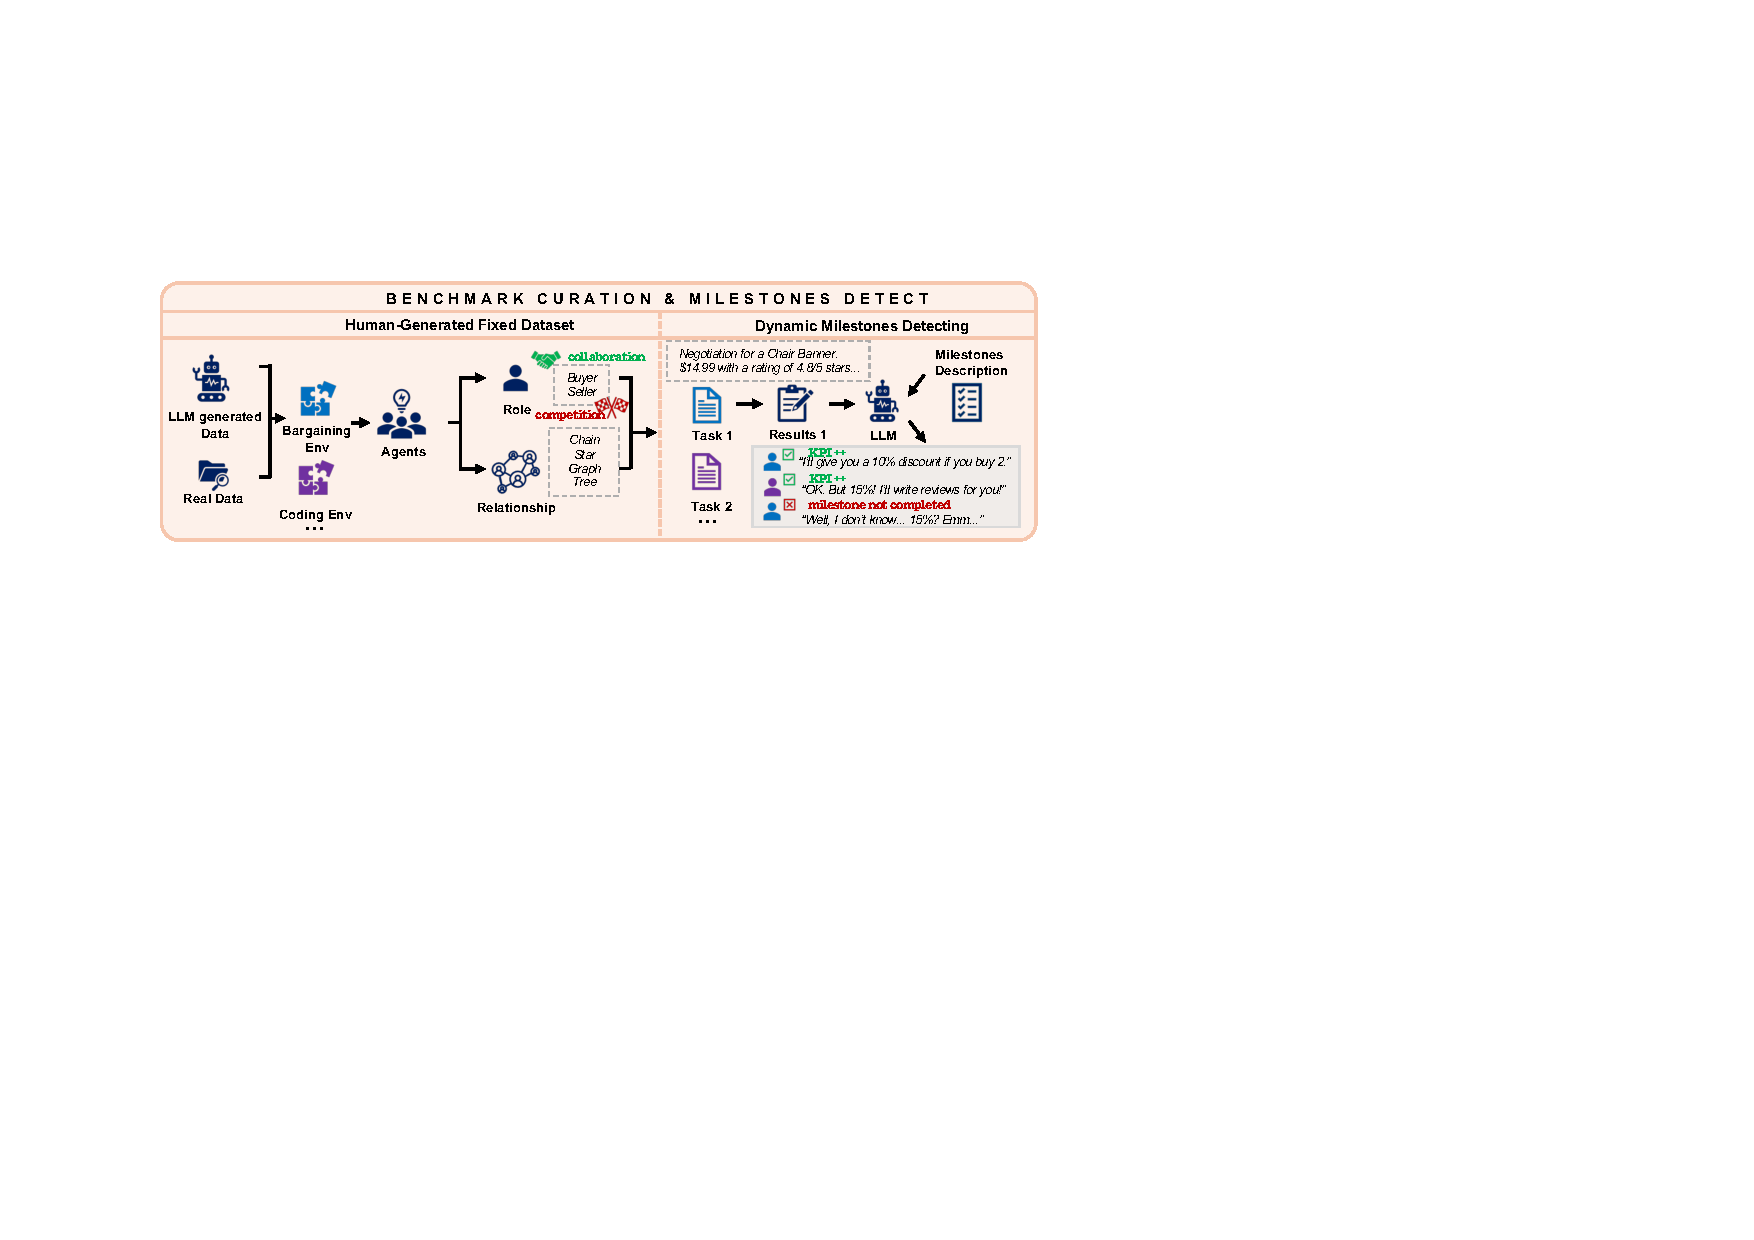
\includegraphics[width=\textwidth]{graphs/marble_graph.pdf}
    \caption{우리의 benchmark curation과 KPI metric을 위한 dynamic milestone detection의 예시.}
    \label{fig:method}
\end{figure*}

우리의 다중 에이전트 프레임워크를 체계적으로 평가하기 위해, \textit{task-oriented} 및 \textit{social-simulation-based} 환경을 포괄하는 다양한 시나리오의 벤치마크를 구성한다(Figure~\ref{fig:overview}). 이 시나리오는 다음의 조합으로 만들어진다. (1) database error analysis, research collaboration처럼 선행 연구나 데이터셋에서 각색한 \textit{기존 다중 에이전트 과제}. (2) Werewolf와 Bargaining처럼 인간 검증과 수정을 거친 \textit{LLM-generated tasks}.
이 이중 접근은 확립된 과제를 활용해 현실성을 보장하고 생성적 확장을 통해 새로움을 제공하며, 인간 검증은 각 시나리오가 일관되고 실행 가능하게 유지되도록 보장한다.

\paragraph{Agents with Mutual Goal.}
task-oriented 시나리오에서 에이전트들은 하나의 특정 과제를 완료한다는 공통 목표를 공유한다. 우리는 네 가지 대표 과제에 초점을 맞춘다. (1) \textbf{research tasks}는 \textit{ResearchTown}~\cite{yu2024researchtownsimulatorhumanresearch}의 설정을 따르며, 상호보완적인 research profile을 가진 에이전트들이 선택된 주제에 대한 새 제안서를 공동 작성한다. (2) \textit{Minecraft-based building tasks}는 공유 환경에서 에이전트들이 구조물을 협력하여 건설하도록 요구한다. (3) \textbf{database error analysis}는 정확히 다섯 에이전트를 포함하며, 각 에이전트는 시스템 불일치의 서로 다른 root cause 진단에 특화된다. (4) \textbf{coding challenges}는 집단적 문제 해결과 software module 개발을 요구한다. 이 과제들 전반에서 에이전트는 효율적으로 조정하고, 일을 나누며, 산출물을 종합해야 한다. 우리는 research topic, Minecraft creation, database error, coding objective의 변형을 포함하여 과제별 100개 test case를 만들어 scenario diversity를 확장한다.

\paragraph{Agents with Conflicting Goals.}
social-simulation based 시나리오에서는 \textbf{Werewolf}와 \textbf{Bargaining} 시나리오를 도입하여 경쟁 요소를 강화한다. Werewolf에서는 두 에이전트 그룹이 사전에 정의된 narrative 안에서 기만 전략을 사용하며 적대적 환경에서 대립한다. Bargaining 환경은 공유 자원에 대한 협상을 시뮬레이션하며, 에이전트는 전략적 양보나 alliance를 통해 개인 이익을 극대화하려 한다. 두 설정은 불확실성 아래에서 adaptability, conflict resolution, negotiation skill을 평가한다.

\paragraph{Role Assignments and Graph Structures.}
다중 에이전트 협업을 강조하기 위해 각 시나리오는 project manager, domain expert, technical specialist 같은 구별된 agent role을 강제하고, star, tree, chain, mesh 같은 특정 graph relationship을 정의한다. 이러한 구조는 현실적인 team dynamics 또는 competition을 반영하며, 에이전트가 정보를 공유하고 의사결정을 내리고 행동을 조정하는 방식을 안내한다.

\paragraph{Milestones Generation for Scenarios}
\label{para:milestones}
MARBLE iteration의 평가를 용이하게 하기 위해 각 과제는 일련의 유연한 milestone으로 분할된다. 경직된 checkpoint와 달리 이러한 milestone은 넓게 정의된다. 예를 들어 research task에서는 research proposal을 위한 다섯 가지 핵심 query(5q)를 완료하거나(자세한 내용은 Appendix~\ref{app:research-scenario} 참조), 이전 5q 집합을 개선함으로써 milestone에 도달할 수 있다. MARBLE의 반복 과정 전반에서 language model은 milestone \(m_1, m_2, \dots\)의 달성 여부를 지속적으로 감시하고 결과를 기록한다. 이 방법은 인간 또는 LLM이 생성한 outline을 dynamic execution-based assessment와 통합하여 중간 진행과 팀 조정이 모두 효과적으로 측정되도록 한다.

% More detailed environment setups, interaction tools, and additional examples for diifernt scenarios appear in Appendix~\ref{app:research-scenario},
% Appendix~\ref{app:werewolf_env},
% and Appendix~\ref{app:database-scenario},
% Appendix~\ref{app:coding-scenario},
% Appendix~\ref{app:bargaining-scenario},
% Appendix~\ref{app: minecraft-scenario} .

서로 다른 scenario에 대한 더 자세한 environment setup, interaction tool, additional example은 Appendix~\ref{app:research-scenario}, ~\ref{app:werewolf_env}, ~\ref{app:database-scenario}, ~\ref{app:coding-scenario}, ~\ref{app:bargaining-scenario}, ~\ref{app: minecraft-scenario}에 제시되어 있다.

% More detailed environment setups, interaction tools, and additional examples for different scenarios appear in Appendix~\cref{app:research-scenario, app:werewolf_env, app:database-scenario, app:coding-scenario, app:bargaining-scenario, app: minecraft-scenario}.

% This process ensures that the generated milestones are specific, achievable, and aligned with the overall task objectives. The integration of large language models, such as GPT-4, allows for iterative refinement and human revision, resulting in high-quality, structured task decompositions. The chain of thought methodology further enhances the coherence and logical progression of milestones, providing a robust foundation for evaluating multi-agent coordination and performance.


% \subsection{Evaluation Metrics}

% The evaluation focuses on two primary dimensions: task completion performance and coordination quality. Task completion metrics measure milestone success rates and global Key Performance Indicators (KPIs). Given MM milestones, each with a success rate SiS_i:
% \[
% \text{KPI} = \frac{\sum_{i=1}^{M} S_i}{M}.
% \]
% These SiS_i values can be derived from automated evaluations such as comparing produced research outcomes against ground-truth references, checking correctness in coding tasks, or computing negotiation efficiency in Bargaining scenarios. Additional resource-based metrics, such as token usage per completed task, provide further insights:
% \[
% E_\text{tokens} = \frac{\text{Total Tokens Used}}{\text{Total Tasks Completed}}.
% \]

% Coordination metrics quantify communication and planning quality. Let CitC_{it} denote the communication content at iteration tt of task ii, and PitP_{it} represent the corresponding planning decisions. A language model evaluation scores each dimension on a scale of 1 to 5, where effective communication is judged by clarity of expression, consistency in role assignments, and assistance in resolution, while effective planning is evaluated by the organization of tasks, the soundness of reasoning, and the suitability of proposed actions. If Qcomm,iQ_{\text{comm},i} and Qplan,iQ_{\text{plan},i} represent averaged communication and planning scores for task ii:
% \[
% Q_{\text{comm},i} = \frac{1}{T_i} \sum_{t=1}^{T_i} q_{\text{comm},it}, \quad Q_{\text{plan},i} = \frac{1}{T_i} \sum_{t=1}^{T_i} q_{\text{plan},it},
% \]
% where TiT_i is the total number of iterations for task ii, and qcomm,it,qplan,it∈{1,…,5}q_{\text{comm},it}, q_{\text{plan},it} \in \{1,\dots,5\} are iteration-level scores. The final coordination metric for a given task integrates these communication and planning scores:
% \[
% S_{\text{coord},i} = \frac{Q_{\text{comm},i} + Q_{\text{plan},i}}{2}.
% \]

\subsection{평가 지표}
\label{sec:eval_metrics}
Figure~\ref{fig:overview}(b)(c)에 나타난 것처럼, 우리의 평가는 두 가지 주요 차원인 \textbf{Task Completion Performance}와 \textbf{Coordination}을 고려한다.

\paragraph{Task Completion Metrics.}
% As described in the paragraph~\ref{para:milestones} section, each task is segmented into a series of flexible milestones, denoted by \(m_1, m_2, \dots, m_M\). An LLM-based detector continuously monitors the iterative process to determine which milestones have been achieved and records the corresponding list of contributing agents. For example, if agent \(j\) contributes to \(n_j\) milestones out of the total \(M\), their individual KPI is computed as \(n_j/M\), with the overall KPI being the average of these individual KPIs across all agents. \kunlun{prmopt refer to appendix}

Section~\ref{para:milestones}에서 설명했듯이 각 과제는 일련의 유연한 milestone으로 분할된다. LLM 기반 detector는 반복 과정을 지속적으로 감시하여 어떤 milestone이 달성되었는지 식별하고 해당 기여 에이전트를 기록한다. 각 에이전트에 대해 그 에이전트가 기여한 milestone 수를 \(n_j\)로 표기하며, 개별 KPI는 \(n_j\)와 전체 milestone 수 \(M\)의 비율로 계산한다. 전체 KPI는 모든 \(N\)개 에이전트의 개별 KPI 평균으로 정의되며, 다음과 같이 계산된다.
\[
\text{KPI}_{\text{overall}} = \frac{1}{N}\sum_{j=1}^{N}\text{KPI}_j = \frac{1}{NM}\sum_{j=1}^{N} n_j.
\]

Milestone detection에서 도출한 KPI 외에도 최종 산출물 품질을 평가하기 위해 별도의 \textbf{task-based score}를 계산한다. Research 또는 bargaining 같은 과제에는 LLM이 정의한 scoring rubric을 적용해 점수를 생성하고, Minecraft, Werewolf, database error fix, coding 같은 과제는 accuracy와 같은 rule-based metric으로 평가한다. 이러한 task-based assessment를 위한 자세한 scoring criteria와 evaluation prompt는 각각 Appendix~\ref{app: minecraft-scenario}, ~\ref{app:werewolf_env}, ~\ref{app:database-scenario}, ~\ref{app:coding-scenario}에 제공되며, 조정 능력을 평가하면서 지표의 효과를 보여 준다.

\paragraph{Coordination Metrics.}
Coordination은 에이전트의 communication 및 planning capability를 정량화하여 평가한다. \textbf{Communication Score}(\(C_{\text{score}}\))는 task description, agent profile, aggregated communication data 같은 입력을 고려하는 LLM 기반 평가에서 도출되며, 다섯 점 척도의 점수를 산출한다(communication이 없으면 \(C_{\text{score}} = 0\)). 유사하게 \textbf{Planning Score}(\(P_{\text{score}}\))는 agent profile과 aggregated planning data를 바탕으로 과제를 조직하고 역할을 유지하며 전략을 적응시키는 능력을 다섯 점 척도로 평가해 결정된다. 전체 \textbf{Coordination Score}(\textbf{CS})는 이 두 하위 점수의 평균으로 계산된다. 평가 과정과 출력 형식에 대한 자세한 내용은 Appendix~\ref{sec:important-prompts}에 제공된다. 또한 우리는 이러한 지표와 인간 판단의 정렬을 비교하는 human evaluation을 수행했으며, 결과는 Appendix~\ref{app:human-evaluation}에 있다.


% \subsection{Evaluation Metrics}
% \label{sec:eval_metrics}

% As illustrated in Figure~\ref{fig:overview}(b)(c) , our evaluation considers two primary dimensions: \textbf{Task Completion Performance} and \textbf{Coordination}.

% \paragraph{Task Completion Metrics.}
% We decompose each task into $M$ milestones, each with a binary success indicator $s_i$. The overall task completion metric (\textbf{KPI}) is:
% \[
% \text{KPI} = \frac{\sum_{i=1}^{M} s_i}{M}.
% \] \kunlun{redefine the annotation expand the }
% At the conclusion of a task round, we identify which agents contributed to each successful milestone and increment their individual scores. Each agent’s KPI is then its total successful contributions divided by the total completed milestones. The average KPI across $N$ agents is:
% \[
% \text{Average KPI} = \frac{\sum_{j=1}^{N} \text{KPI}_j}{N}.
% \]
% This KPI captures both inter-agent competition and collective efficiency. Depending on the specific task, success may be measured via GPT-based scoring of final outputs (e.g., for research proposals) or direct accuracy (e.g., for database error fixes). Details for each scenario are provided in the Appendix.

% \paragraph{Collaboration \& Competition Metrics.}

% We adopt an arena-based comparison framework \citep{DBLP:conf/icml/ChiangZ0ALLZ0JG24} to evaluate multi-agent models on both coordination and competitive capabilities. For each pair of models $m_i$ and $m_j$, we conduct $R$ independent matchups on the same task.
% In each matchup $r$, two key scores are assigned via LLM-based evaluation: a Communication Score, $C_{m_i}^r$, and a Planning Score, $P_{m_i}^r$.
% \heng{I don't understand what independent matchups or matchup means}

% \begin{itemize}
%     \item \textbf{Communication Score} ($C_{\text{score}}$): Assesses clarity, relevance, and effectiveness of information exchange. If no communication occurs, $C_{\text{score}} = 0$.
%     \item \textbf{Planning Score} ($P_{\text{score}}$): Evaluates how well the agents organize tasks, maintain roles, and adapt strategies.
% \end{itemize}

% For each task $i$, we collect $C_{\text{score},i}$ and $P_{\text{score},i}$ over the entire interaction. The \textbf{Coordination Score} is then:
% \[
% S_{\text{coord},i} \;=\; \frac{C_{\text{score},i} + P_{\text{score},i}}{2}.
% \]

% These scores, which range from 1 to 5 (with a score of 0 assigned if no communication occurs), are averaged to compute an overall Arena Score for model $m_i$:
% \[
% A_{m_i} = \frac{1}{R}\sum_{r=1}^R \left(\frac{C_{m_i}^r + P_{m_i}^r}{2}\right).
% \] \kunlun{too basic change}
% In head-to-head comparisons, the model with the higher Arena Score is declared the winner, and each model's win rate is computed as the fraction of matchups it wins over all its comparisons. This arena-based approach, commonly used in recent studies \citep{DBLP:conf/icml/ChiangZ0ALLZ0JG24,chen-etal-2024-llmarena, zhou2024webarena}, robustly captures both collaborative and competitive dynamics that traditional task-based metrics—such as accuracy or final output quality—often overlook.


% \kunlun{adding arena based settings}
% \kunlun{specifying the KPI is actually the inter competition metrics}
% As shown in Figure~\ref{fig:overview}, our evaluation focuses on two primary dimensions: \textbf{Task Completion Performance} and \textbf{Coordination Quality }

% \textbf{Task Completion Metrics.} These metrics measure milestone success rates and global Key Performance Indicators (\textbf{KPIs}). For a task involving $M$ milestones, where each milestone has a success rate $S_i$, the overall KPI is computed as:
% \[
% \text{KPI} = \frac{\sum_{i=1}^{M} S_i}{M}.
% \]
% At the end of each task round, we first determine whether the milestones $M$ are completed. If completed, the system identifies the contributing Agents and increments their individual scores by 1. Each agent's KPI is then calculated as their total contributions divided by the total completed milestones. Finally, the average KPI across all agents is:
% \[
% \text{Average KPI} = \frac{\sum_{j=1}^{N} \text{KPI}_j}{N},
% \]
% \kunlun{strengthen the KPI evaluates the inter-competition among agents a good way to evaluate how scaling of number of agents will be useful in the more efficience view, KPI will sever both an task evaluation and inter-competition evaluation method}
% where $N$ is the number of agents. This metric provides a quantitative measure of the overall contribution of agents within the coordination framework. It effectively evaluates the average agent's participation and efficiency in the current structure or collaboration mode.

% For additional insights, resource-based metrics such as Token Usage are defined as:
% \[
% E_\text{tokens} = \frac{T_\text{tokens}}{T_\text{Iter}},
% \]
% where $T_\text{tokens}$ represents the total number of tokens used, and $T_\text{Iter}$ denotes the total number of iterations.
% \kunlun{don't need the formula for the tokens calculation}
% \textbf{Coordination and Competition Metrics.}
% \kunlun{We evaluate the multi-agent group level coordination and competition ability according to the communications between agents and their planning for the next round for each of the agent}

% \kunlun{to clarify we are using the arena based evaluation combining the specific scoring for the two part, the prompt will include two models communications or planning of the whole tasks and then the gpt will first score them and then compare them, so each model will compete with other model, we will calculate the winrate and each win will score them in 1 point so then they will have the final coordination/competition point}

% These metrics quantify the quality of \textbf{Communication} and \textbf{Planning}. Let $C_{it}$ denote the communication content and $P_{it}$ the planning decisions at iteration $t$ of task $i$. Evaluations are conducted on each dimension using a 1-5 scale, with scores derived from GPT-4o prompts.

% \textbf{Communication Score} ($q_{\text{comm},it}$): This evaluates the effectiveness of information transmission, clarity of expression, and assistance in task resolution.
% \kunlun{if there is no communication the communication score will be zero}
% \textbf{Planning Score} ($q_{\text{plan},it}$): This assesses task organization and clarity in role maintenance.

% For task $i$ with $T_i$ iterations, the averaged communication and planning scores are:
% \[
% Q_{\text{comm},i} = \frac{1}{T_i} \sum_{t=1}^{T_i} q_{\text{comm},it}\]

% \[\quad Q_{\text{plan},i} = \frac{1}{T_i} \sum_{t=1}^{T_i} q_{\text{plan},it},
% \]
% where $q_{\text{comm},it}, q_{\text{plan},it} \in \{1,\dots,5\}$.

% The overall \textbf{Coordination Score} for task $i$ is the average of these two dimensions:
% \[
% S_{\text{coord},i} = \frac{Q_{\text{comm},i} + Q_{\text{plan},i}}{2}.
% \]

% This comprehensive evaluation framework ensures a holistic assessment of agent coordination, emphasizing both task success and the quality of collaboration.


% \subsection{Coordination Methods}

% The system supports multiple coordination protocols that reflect varying degrees of centralized or decentralized planning, as illustrated in Figure~????????????????????????????????????????????????????????????????????????????????????????????????????????????????????????????????????????????????????????????????????????????????????????????????\ref{fig:overview}. A star configuration involves a central planner agent connected to all actors, distributing tasks and integrating feedback. A tree configuration establishes a hierarchical decision-making structure, with a top-level planner and subsequent layers of subordinate agents. More decentralized protocols, such as graph or chain patterns, promote self-planning and iterative information flow among agents without a single controlling entity.

% Within each chosen structure, several techniques enhance coordination and adaptability. Group discussions facilitate role clarification, resource sharing, and consensus building. Self-evolving planning leverages iterative feedback loops, refining strategies based on prior outcomes. Multi-head search tree planning explores multiple solution candidates in parallel, selecting the most promising ones. Historical experiences are continuously distilled into summarized insights, enabling the agents to learn from past iterations. Advanced reasoning techniques, including chain-of-thought and reflection prompts, support a deeper understanding of complex tasks. Furthermore, agents may internally simulate world models or future trajectories to anticipate potential risks, improve planning accuracy, and reduce trial-and-error. These combined mechanisms ensure that the system dynamically refines its strategies, fosters robust collaboration, and ultimately improves both task completion performance and coordination quality.


% We explore a spectrum of coordination protocols characterized by distinct structural configurations, ranging from fully centralized planning to more decentralized, agent-centric approaches. In particular, we consider four primary structural paradigms---\textbf{star}, \textbf{tree}, \textbf{graph}, and \textbf{chain}---as well as corresponding methodological enhancements that dynamically refine task planning and execution.

% \paragraph{Structure-Based Coordination Protocols.}
% In the \textbf{star} configuration, a single central planner agent is connected to all other agents. This planner assigns tasks to each agent and aggregates their feedback, utilizing it to refine subsequent planning rounds. The \textbf{tree} configuration instead organizes agents hierarchically: a top-level planner agent orchestrates a set of child agents, each of which may recursively plan for its own subordinates. This hierarchy engages in iterative feedback loops, with information and planning updates flowing up and down the structure.

% More decentralized paradigms, such as the \textbf{graph} structure, rely on a network of interconnected agents that exchange information and coordinate tasks without a single controlling entity. We consider several variants of graph-based coordination, including \textbf{mesh}, \textbf{layered}, and \textbf{random} topologies, each facilitating concurrent planning, flexible communication pathways, and distributed decision-making. In contrast, the \textbf{chain} configuration arranges agents in a linear sequence, where an initial agent selects subsequent agents and tasks in a pipeline fashion. Each round involves a single agent taking action, thereby propagating decision-making along the chain.

% \paragraph{Planner Design and Enhancement Techniques.}
% Building upon these structural configurations, we further refine coordination through advanced planner design and iterative adaptation methods. Starting from the star structure as a baseline, we introduce a zero-shot chain-of-thought prompt design, whereby the planner is provided with the target task, each agent’s profile, and a distilled history of completed subtasks. This allows the planner to reason step-by-step and produce carefully orchestrated task assignments for each agent in the current round. We also employ a \textbf{REACT}-style reasoning approach, which interleaves reasoning and acting steps, enabling the planner to dynamically adjust strategies as it observes intermediate outcomes and feedback.

% Additionally, \textbf{group discussions} at each round allow every agent to express its perspectives, resource constraints, and role suggestions. The planner then integrates these contributions to refine the allocation of tasks, ensuring that the final plan reflects a consensus-driven division of labor. Furthermore, we incorporate \textbf{cognitive planning} principles inspired by management heuristics, emphasizing effective workload distribution, skill utilization, and balanced task assignments. After each round, the planner generates a concise summary of lessons learned, capturing historical insights that guide subsequent planning iterations. Over time, these adaptive processes accumulate a rich reservoir of experience, enabling the system to continuously refine its decision-making, reduce coordination overhead, and enhance both performance and overall collaboration quality.

% We propose a streamlined framework that integrates structural coordination with adaptive planning enhancements. Our approach considers four primary configurations---\textbf{star}, \textbf{tree}, \textbf{graph}, and \textbf{chain}---which can be grouped by their degree of centralization. Specifically, \textbf{star} and \textbf{tree} are centralized methods where one (or a hierarchy of) planner(s) manages task allocation and aggregates feedback, while \textbf{graph} and \textbf{chain} rely on decentralized coordination through peer-to-peer interactions and sequential task handoffs.

% \paragraph{Centralized Coordination: Star \& Tree.}
% In the \textbf{star} configuration, a single central planner assigns tasks to all agents and consolidates their feedback, making it effective for tasks that require strong oversight but potentially limited in scalability. The \textbf{tree} structure builds on this by organizing agents hierarchically: a top-level planner delegates tasks to subordinate planners, combining centralized control with enhanced scalability for complex tasks.

% \paragraph{Decentralized Coordination: Graph \& Chain.}
% The \textbf{graph} configuration utilizes a network of interconnected agents that communicate directly, enabling concurrent planning and distributed decision-making. In contrast, the \textbf{chain} structure arranges agents sequentially, where each agent passes decisions to the next. This approach is well-suited for tasks with sequential dependencies, though it may constrain parallel processing.

% \paragraph{Planner Design and Enhancements.}
% \kunlun{updating the new method of cognitive evolving with expectation result and experience update for better task  planning }
% \kunlun{for the star coordination style, ablation on different planning stratigies}
% Building on these structures, our approach employs iterative, feedback-driven planning. A zero-shot chain-of-thought prompt equips the planner with the target task, agent profiles, \heng{not sure what agent profile contains, define and give example} and a summary of past subtasks, enabling step-by-step reasoning. The REACT-style mechanism interleaves planning with action, while \textbf{group discussions} allow agents to share insights and constraints. \textbf{Cognitive planning} principles further ensure effective workload distribution and task alignment. Each round concludes with a concise summary of lessons learned, continuously refining the system's coordination and performance.

% % \input{sections/4_verification}

% \heng{It would be interesting to show the impact of competition, the impact of coordinator agent, the impact of various communication protocles etc. through ablation tests. Have you thought about adding more levels of managers in star graph? perhaps future work?}

% \heng{The current analysis sections are bit tedious. try to add insights and findings instead of repeating numbers from the result tables. add some qualitative analysis and examples}

% \begin{table*}[h!]
% \centering
% \resizebox{\linewidth}{!}{
% \begin{tabular}{
%     l
%     | >{\columncolor{ResearchColor}}S[table-format=3.2] >{\columncolor{ResearchColor}}S[table-format=3.2]
%     | >{\columncolor{MinecraftColor}}S[table-format=4.2] >{\columncolor{MinecraftColor}}S[table-format=5.2]
%     | >{\columncolor{DatabaseColor}}S[table-format=4.2] >{\columncolor{DatabaseColor}}S[table-format=5.2]
%     | >{\columncolor{CodingColor}}S[table-format=4.2] >{\columncolor{CodingColor}}S[table-format=5.2]
%     | >{\columncolor{BargainingColor}}S[table-format=4.2] >{\columncolor{BargainingColor}}S[table-format=5.2]
%     | >{\columncolor{WereWolfColor}}S[table-format=6.3] >{\columncolor{WereWolfColor}}S[table-format=5.2]
% }
% \toprule
% \multirow{2}{*}{\textbf{Model}} 
% & \multicolumn{2}{c}{\textbf{Research}} 
% & \multicolumn{2}{c}{\textbf{Minecraft}}
% & \multicolumn{2}{c}{\textbf{Database}}
% & \multicolumn{2}{c|}{\textbf{Coding}}
% & \multicolumn{2}{c}{\textbf{Bargaining}}
% & \multicolumn{2}{c}{\textbf{WereWolf}} \\
% \cmidrule(lr){2-3}\cmidrule(lr){4-5}\cmidrule(lr){6-7}\cmidrule(lr){8-9}\cmidrule(lr){10-11}\cmidrule(lr){12-13}
% & \textbf{TS} & \textbf{CS}
% & \textbf{TS} & \textbf{CS}
% & \textbf{TS} & \textbf{CS}
% & \textbf{TS} & \textbf{CS}
% & \textbf{TS} & \textbf{CS}
% & \textbf{TS} & \textbf{CS} \\
% \midrule
% \textbf{Meta-Llama-3.1-8B}
%  & 80.87 & 52.40
%  & 6.12 & 54.40
%  & 0.00 & 61.92
%  & 59.90 & 67.24
%  & 72.81 & 73.36
%  & 12.635 & 60.00 \\

% \textbf{Meta-Llama-3.1-70B}
%  & 80.80 & 49.50
%  & 0.21 & 75.00
%  & 3.20 & 40.20
%  & 62.10 & 67.18
%  & 72.13 & 71.46
%  & 19.82 & 60.60 \\

% \textbf{Meta-Llama-3.3-70B}
%  & 80.00 & \textbf{72.00}
%  & 9.15 & 69.00
%  & 1.30 & 41.70
%  & 56.60 & 74.40
%  & 73.15 & 69.56
%  & \textbf{36.325} & \textbf{76.30} \\
% \midrule
% \textbf{gpt3.5-turbo}
%  & 70.20 & 55.90
%  & 5.05 & 63.60
%  & 2.30 & \textbf{59.62}
%  & 55.50 & \textbf{76.20}
%  & 71.67 & 72.00
%  & 15.685 & 75.90 \\

% \textbf{gpt-4o-mini}
%  & \textbf{84.13} & 52.00
%  & \textbf{33.60} & 61.50
%  & 2.70 & 39.60
%  & \textbf{65.10} & 66.30
%  & \textbf{74.47} & \textbf{74.20}
%  & 14.06 & 60.10 \\
% \bottomrule
% \end{tabular}
% }

\begin{table*}[h!]
\centering
\renewcommand{\arraystretch}{1.2}  % 调整行距
\setlength{\tabcolsep}{8pt}  % 调整列间距
\resizebox{\linewidth}{!}{
\begin{tabular}{
    l
    |>{\columncolor{ResearchColor}}c>{\columncolor{ResearchColor}}c
    |>{\columncolor{MinecraftColor}}c>{\columncolor{MinecraftColor}}c
    |>{\columncolor{DatabaseColor}}c>{\columncolor{DatabaseColor}}c
    |>{\columncolor{CodingColor}}c>{\columncolor{CodingColor}}c
    |>{\columncolor{BargainingColor}}c>{\columncolor{BargainingColor}}c
    |>{\columncolor{WereWolfColor}}c>{\columncolor{WereWolfColor}}c
}
\toprule
\multirow{2}{*}{\textbf{Model}} 
& \multicolumn{2}{c}{\textbf{Research}} 
& \multicolumn{2}{c}{\textbf{Minecraft}}
& \multicolumn{2}{c}{\textbf{Database}}
& \multicolumn{2}{c|}{\textbf{Coding}}
& \multicolumn{2}{c}{\textbf{Bargaining}}
& \multicolumn{2}{c}{\textbf{WereWolf}} \\
\cmidrule(lr){2-3}\cmidrule(lr){4-5}\cmidrule(lr){6-7}\cmidrule(lr){8-9}\cmidrule(lr){10-11}\cmidrule(lr){12-13}
& \textbf{TS} & \textbf{CS}
& \textbf{TS} & \textbf{CS}
& \textbf{TS} & \textbf{CS}
& \textbf{TS} & \textbf{CS}
& \textbf{TS} & \textbf{CS}
& \textbf{TS} & \textbf{CS} \\
\midrule
\textbf{Meta-Llama-3.1-8B}
 & 80.87 & 52.40
 & 6.12 & 54.40
 & 34.00 & 40.00
 & 59.90 & 67.24
 & 72.81 & 73.36
 & 12.64 & 60.00 \\

\textbf{Meta-Llama-3.1-70B}
 & 80.80 & 49.50
 & 0.21 & 75.00
 & \textbf{53.00} & 37.70
 & 62.10 & 67.18
 & 72.13 & 71.46
 & 19.82 & 60.60 \\

\textbf{Meta-Llama-3.3-70B}
 & 80.00 & \textbf{72.00}
 & 9.15 & 69.00
 & 28.50 & 40.00
 & 56.60 & 74.40
 & 73.15 & 69.56
 & \textbf{36.33}  & \textbf{76.30} \\
\midrule
\textbf{gpt3.5-turbo}
 & 70.20 & 55.90
 & 5.05 & 63.60
 & 45.00 & \textbf{60.89}
 & 55.50 & \textbf{76.20}
 & 71.67 & 72.00
 & 15.69 & 75.90 \\

\textbf{gpt-4o-mini}
 & \textbf{84.13} & 52.00
 & \textbf{33.60} & 61.50
 & 45.00 & 43.22
 & \textbf{65.10} & 66.30
 & \textbf{74.47} & \textbf{74.20}
 & 14.06 & 60.10 \\
\bottomrule
\end{tabular}
}
\caption{\textbf{Average Task Score} (\textbf{TS}) (\%) and the Coordination Score (\textbf{CS}) for Minecraft, Database, Coding, Bargaining, and WereWolf, scores are multiplied by 20. We can see that model abilities are still the key factor for task completion. CS is a good indicator for TS given three pairs of scenarios having the one model having the highest TS and CS at the same time.
}
\label{tab:avg_task_score}
\end{table*}





    % \begin{table*}[h]
    % \centering
    % \begin{tabular}{
    %     l      % Agents Protocol
    %     | S[table-format=1.3]   % Planning
    %      S[table-format=1.3]   % Communication
    %     | S[table-format=1.3]   % KPI
    %      S[table-format=6.2]   % Token Usage
    %      S[table-format=1.3]   % Task Score
    % }
    % \toprule
    % \multirow{2}{*}{\textbf{Coordination Protocol}} & \multicolumn{2}{c|}{\textbf{Coordination Score}} & \multicolumn{3}{c}{\textbf{Task Completion}} \\
    % \cmidrule(lr){2-3} \cmidrule(lr){4-6}
    %  & \textbf{Planning} & \textbf{Communication} & \textbf{KPI} & \textbf{Token Usage} & \textbf{Task Score} \\
    % \midrule
    % \rowcolor{yellow!20} \multicolumn{6}{c}{\textit{Research}} \\
    % \midrule
    
    % \rowcolor{blue!10} Graph-Mesh   & 4.369 & 4.200       & 0.755           & 86983     & 4.238          \\
    % \rowcolor{blue!10} Star   & \textbf{4.680} &  \textbf{4.786}    &      0.707      &   31365   &    4.227       \\
    % \rowcolor{blue!10} Chain     &  4.100 & ——       & ——  &  14833    &  4.240 \\
    % \rowcolor{blue!10} Tree     & 4.100  &  —— &      ——       &  \textbf{11880}    &     \textbf{4.253}      \\
    
    % \bottomrule
    % \end{tabular}
    % \caption{Average Metrics for Research Tasks, Communication and KPI value are currently not available for Chain and Tree due to the current implementation mechanism. \jiaxuan{Add findings - what should readers learn from this?}}
    % \label{tab:research_metrics}
    % \end{table*}








\section{Experiment Setup}
\label{sec:experiment-setup}

\subsection{Experiment Settings}
\paragraph{Models.} Since our MARBLE framework required function-calling abilities. Thus, we consider three open-source models: \textit{Meta-Llama-3.3-70B~\citep{dubey2024llama}}, \textit{Meta-Llama-3.1-70B-Instruct-Turbo~\citep{dubey2024llama}}, and \textit{Meta-Llama-3.1-8B-Instruct-Turbo}, as well as two closed-source models: \textit{GPT-3.5-turbo-0125} and \textit{GPT-4o-mini}\footnote{\href{https://www.openai.com}{https://www.openai.com}}.We access the open-souce models are provided by the \textit{togetherai}~\footnote{\href{https://www.together.ai}{https://www.together.ai}} service, utilizing the default parameter settings. 

For the agent actions, we configure the models with a maximum token number (\texttt{max\_token\_num}) of 1024, a temperature of 0.7, and a top\_p of 1.0, in order to balance the creativity and consistency of the agents' responses during interactions. The overall maximum iterations are set to 5 for research and 20 for Minecraft; more details can be found in the Appendix.  In our evaluation, which involves both Task Completion and Simulation scenarios, we assess the models along two primary axes: \emph{Task Score} (\textbf{TS}) and \emph{Coordination Score} (\textbf{CS}), using the same metrics as described in the Metrics section. The maximum communication iteration number is also set to 5. Furthermore, the long-term base memory for each agent is set to be unlimited. Finally, for the main experiment, a graph-mesh coordination protocol is adopted to facilitate interactions.

%To ensure manageable computational overhead and consistency across all models and tasks, the maximum number of interaction iterations is generally limited to 5; however, for Task Score and Coordination Score evaluations as well as milestone detection, we set the maximum iterations to 40 and fix the temperature to 0.


% \paragraph{Agent Action Parameters.} For the agent actions, we configure the models with the following parameters: maximum token number max\_token\_num set to 1024, temperature set to 0.7, and top\_p set to 1.0. These settings aim to balance the creativity and consistency of the agents' responses during interactions. The overall maximum iterations is set to 5 for research, 20 for Minecraft, and more details could refer to the Appendix \kunlun{appendix}. 


% \kunlun{fix one model while doing the evaluation for the simulation scenario, fix to 4o}
% \paragraph{Evaluation Settings.} Our evaluation involves both Task Completion and Simulation scenarios. In each scenario, we assess the models along two primary axes: \emph{Task Score} (\textbf{TS}) and \emph{Coordination Score} (\textbf{CS})\kunlun{switch to the same as the metric part}. We limit the maximum number of interaction iterations for each evaluation session to 5 to ensure manageable computational overhead and consistency across all models and tasks.\kunlun{4o for TS, CS evaluation, temperature set to 0, 4o for milestones detect}
% \kunlun{unlimit longterm base memory} \kunlun{graph-mesh  coordination protocol for main experiment}

% \paragraph{Benchmark Organization.} Our benchmark is divided into two main categories of tasks: \textit{Task Completion} and \textit{Simulation}. For each category, both the final task result and the associated planning quality are evaluated. To derive a final score for each category, we first compute scenario-specific metrics and then average them. This ensures that each model’s overall performance is represented fairly and comprehensively.

% \paragraph{Memory and Coordination Setup.} In the main experimental configuration, we adopt a \emph{long-term self-memory} approach to allow models to retain and utilize information from earlier interaction turns. Moreover, to better handle complex multi-agent interactions, we employ a \emph{star coordination} strategy: in the simulation scenario, multiple teams (or ``stars'') interact, requiring strategic coordination and information exchange among these entities.


\subsection{Main Experiment One: Model Performance Across Different Scenarios}

% In this experiment, we evaluate the performance of the five models across different scenarios. The results are summarized in Table~\ref{tab:avg_task_score}.

% 1. result 1: gpt-4o-mini show superior results in most of the task; 

% 2. coordination score can some kina affect the task score in cases like,  but not necessarie, one extreme case mine-craft 3.1 70b, refer to \ref{fig:minecraft-function-call}, our explanation is that model abilities matter the most,

In this experiment, we evaluate the performance of five models across diverse scenarios, with results summarized in Table~\ref{tab:avg_task_score}. Our analysis leads to several key insights:

\paragraph{1. Superior Task Performance of \texttt{gpt-4o-mini}:}  
Across multiple tasks, \texttt{gpt-4o-mini} consistently achieves high Task Scores (TS). For example, in the Research scenario it obtains a TS of \textbf{84.13}\%, outperforming other models such as \texttt{Meta-Llama-3.1-8B} (80.87\%) and \texttt{Meta-Llama-3.1-70B} (80.80\%). Similar trends are observed in the Coding domain, where \texttt{gpt-4o-mini} records a TS of 65.10 compared to lower scores from its competitors. These results indicate that the underlying model capabilities are a decisive factor in achieving superior task performance.

\paragraph{2. The Nuanced Role of Coordination (Collaboration) Score:}  
While the Collaboration Score (CS) is designed to measure coordination ability, our findings suggest that its impact on the overall task performance is complex. For instance, in the Minecraft scenario, \texttt{Meta-Llama-3.1-70B} exhibits a high CS of 75.00 but an extremely low TS of 0.21, a more deep analysis for this can refer to Appendix~\ref{fig:minecraft-function-call}. This discrepancy implies that, although coordination contributes to performance, it does not compensate for inherent deficiencies in task execution capabilities. In contrast, models that balance both high TS and moderate-to-high CS—such as \texttt{gpt-4o-mini}—demonstrate more robust and reliable performance across scenarios.

\paragraph{3. Model-Specific Strengths and Context-Dependent Performance:}  
Our results reveal that different models exhibit varied strengths depending on the task. For example, \texttt{Meta-Llama-3.3-70B} shows a notable CS in the Research (72.00) and WereWolf (76.30) tasks, yet its TS lags behind that of \texttt{gpt-4o-mini} in several scenarios. These variations emphasize that no single metric can fully capture a model’s effectiveness; instead, both task-specific abilities and coordination skills must be considered. Overall, our study underscores that while coordination plays a role, the intrinsic model capabilities are the primary drivers of success across diverse tasks.


\subsection{Main Experiment Two: Effects of Collaboration Protocols and Planning Strategies}


% According to Fig ~\ref{fig:coordination_protocol_comparison}, 

% 1. graph is superior in the research scenario best in task and planning, and token usage, star and graph have very similar task score results

% 2. Tree don't perform good in research scenario, high token usage and worst task and coordination score


% Acoording to Fig.~\ref{fig:research_metrics}, 1. Cognitive Evolving planing show case the best Coordination much better than others, demonstrate its effectiveness on elicit multiagent coordination, and achieve similar task score as COT which is the best. 
% 2. counter intuitively the group discussion received the worst in both three of the results, one reason could be if too many people joining in the planning group it actually won't be very effectly, such as in the real society a mall group of people manage the whole organization.

We investigate the impact of different collaboration protocols—Star, Tree, Graph, and Chain—on model performance in the Research scenario. 

According to Fig.~\ref{fig:coordination_protocol_comparison}, the graph-based protocol excels in research scenarios with the best task performance, planning efficiency, and token usage, while both the star and graph protocols yield similar task scores. In contrast, the tree-based protocol performs poorly, with high token consumption and the lowest task and coordination scores. As shown in Fig.~\ref{fig:research_metrics}, Cognitive Evolving Planning demonstrates superior coordination—significantly outperforming the alternatives—and achieves a task score comparable to the best, COT. Counterintuitively, the group discussion method scores the worst across all metrics, possibly because an overly large planning group hinders effectiveness, similar to large organizations in real-world scenarios.


\begin{figure}[htbp]
    \centering
    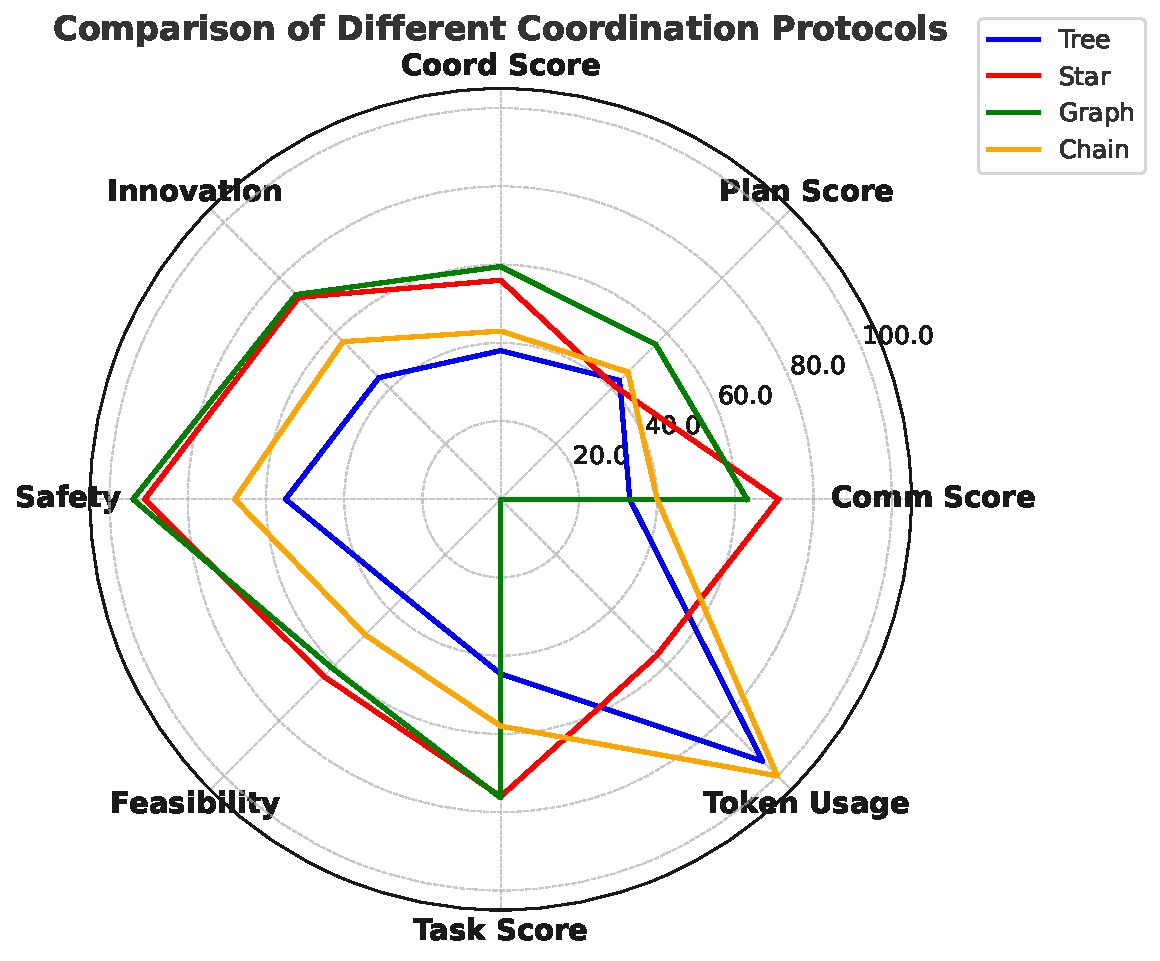
\includegraphics[width=\linewidth]{graphs/comparison_of_coordination_protocols.pdf}
    \caption{Comparison of Different Coordination Protocols.—Tree, Star, Graph, and Chain—across multiple evaluation metrics. Specially, the token usages are scaled such that the lowest value is $0$ and the hightest value is $100$. Details about metrics used for research task can be found at \ref{research_task_metric}}
    \label{fig:coordination_protocol_comparison}
\end{figure}






\begin{figure}[htbp]
    \centering
    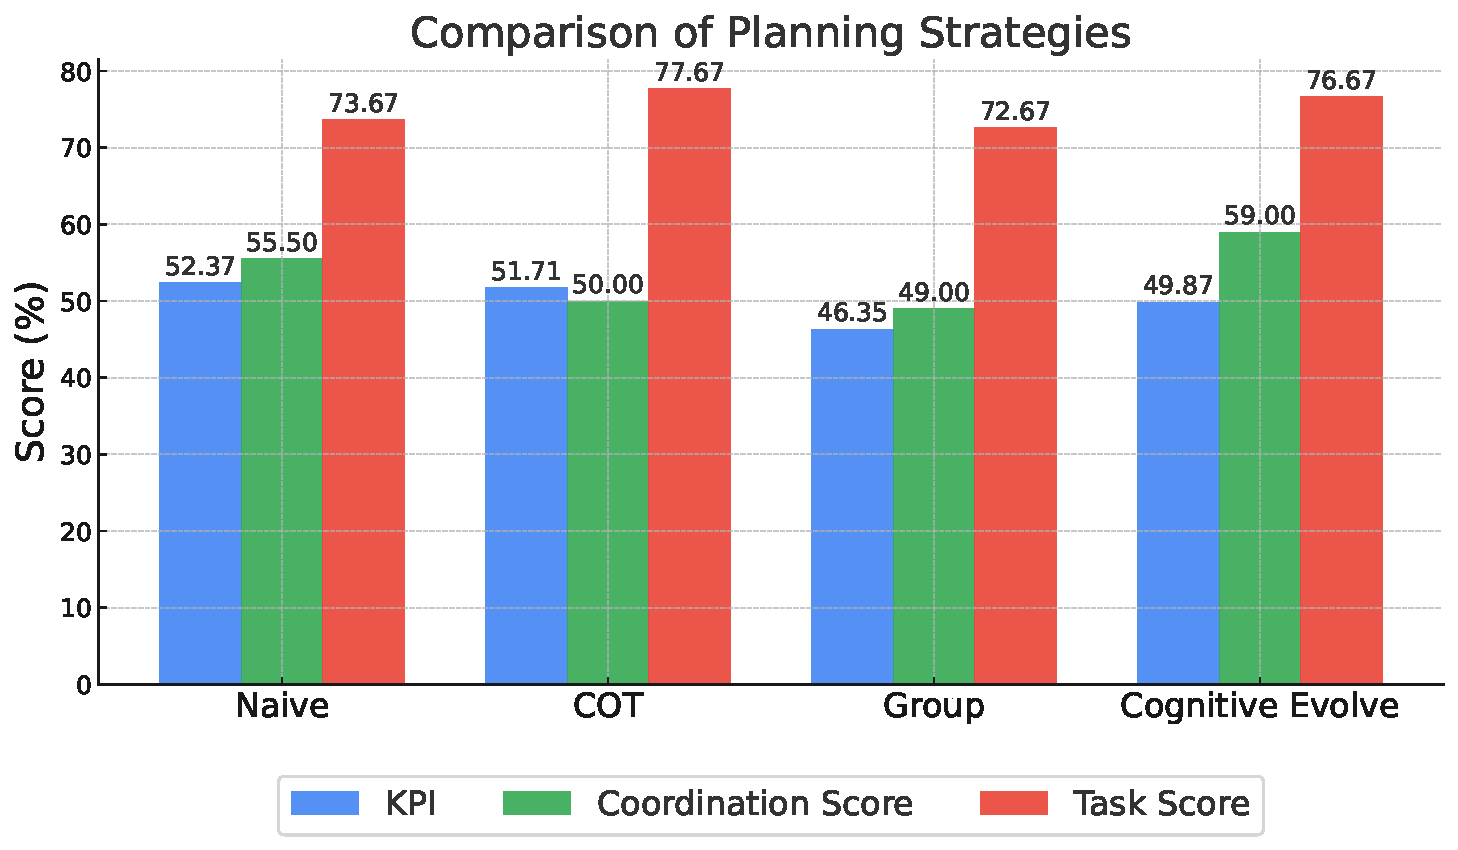
\includegraphics[width=\linewidth]{graphs/research_metrics_legend.pdf}
    \caption{Average Metrics for Research Tasks for different planning prompt strategies. Cognitive Evolve Planning show best result in CS.}
    \label{fig:research_metrics}
\end{figure}

% The \textbf{Cognitive Planning} strategy attains the highest Planning Score (\textbf{4.64}), indicating superior planning abilities. However, the \textbf{Group Discussion} strategy achieves the highest Task Score (\textbf{4.26}), suggesting that collective deliberation among agents enhances task performance.

% The interplay between coordination protocols and planning strategies underscores the importance of selecting appropriate frameworks based on the specific requirements of a task. For instance, tasks that demand high levels of coordination and strategic planning may benefit from centralized protocols like Star coupled with Cognitive Planning strategies. In contrast, tasks prioritizing efficiency and focused execution might be better served by hierarchical protocols like Tree alongside Group Discussion strategies.

\section{Ablation Study}

The goal of our ablation study is to identify the key modules and parameters that affect performance.

\paragraph{Ablation on Different Max Iteration Settings} We evaluate 10 tasks from the Minecraft scenario using six distinct maximum iteration settings. As shown in Fig.~\ref{fig:gpt4o_minecraft_scores}, both task and coordination scores increase from 1 to 7 iterations, but then drop sharply at 10 iterations. At 20 iterations, while the task score shows a recovery, the coordination score remains nearly unchanged beyond 7 iterations. This pattern suggests that, for highly challenging tasks, excessive iterations may lead to coordination degradation—possibly due to communication overhead or conflicting directives emerging over prolonged interactions. These findings underscore the need for adaptive iteration strategies that balance task execution with effective coordination.


\begin{figure}[htbp]
    \centering
    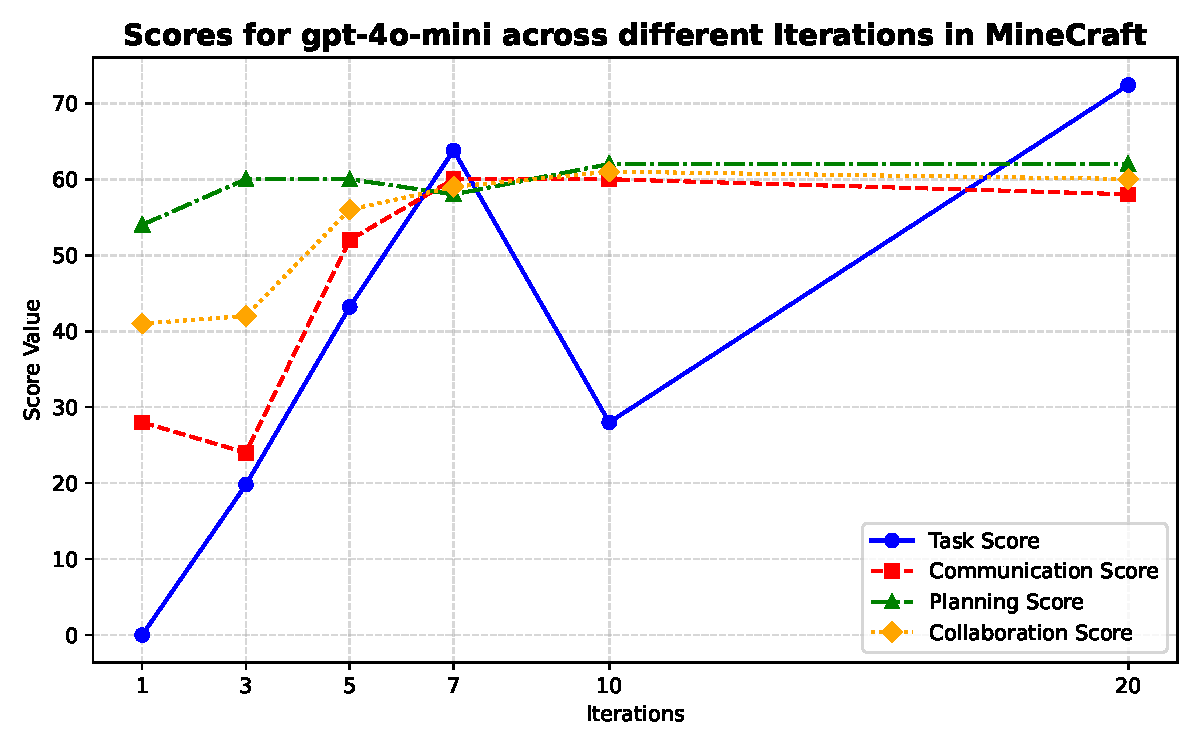
\includegraphics[width=\linewidth]{graphs/scaling_iterations.pdf}
    \caption{Scores for \texttt{gpt-4o-mini} across different iterations in Minecraft. The figure presents Task Score (TS), Communication Score (CS), Planning Score (PS), and Collaboration Score (CoS) over multiple iterations.}
    \label{fig:gpt4o_minecraft_scores}
\end{figure}

\paragraph{Ablation on Different Agent Numbers} We assess configurations with 1, 3, 5, and 7 agents in the research scenario, selecting 20 papers that have at least 7 main authors. As illustrated in Fig.~\ref{fig:scaling_agents}, increasing the number of agents leads to a decrease in the overall KPI, which aligns with the anticipated trade-off between increased collaborative complexity and performance. Notably, the average coordination score improves significantly when moving from 1 to 3 agents, while the average task score increases more gradually. This indicates that a moderate expansion in team size can enhance coordination efficiency, although further increases may introduce additional coordination challenges that counterbalance task performance gains.

\begin{figure}[htbp]
    \centering
    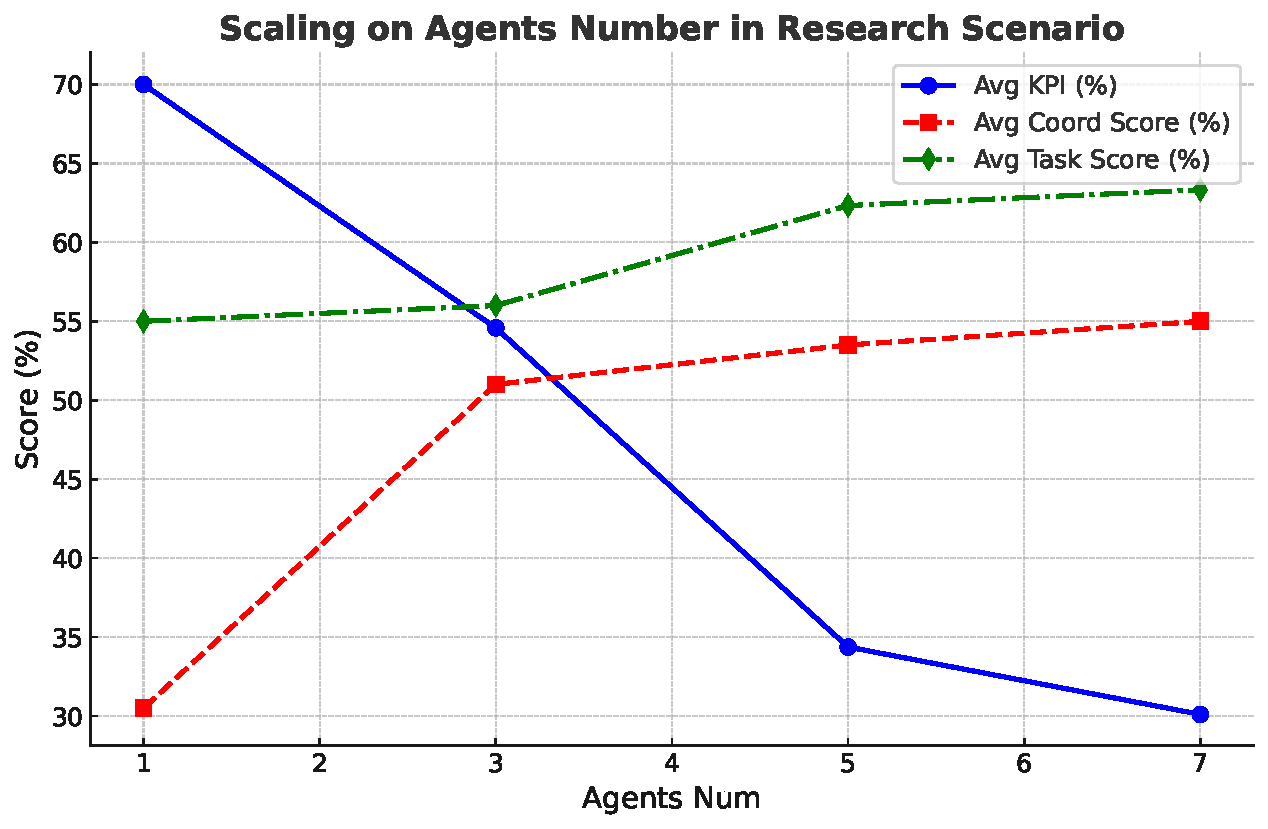
\includegraphics[width=\linewidth]{graphs/scaling_agents_research_scenario.pdf}
    \caption{Scaling on Agents Number in Research Scenario. This figure shows the impact of agent number on KPI, Coordination Score, and Task Score.}
    \label{fig:scaling_agents}
\end{figure}

\section{Emergent Behaviors Analysis}
\label{sec:emergent_behaviors}
In MultiagentBench, goal-driven emergent behaviors are pivotal to team coordination—we argue that these “aha-moments” not only mark when individual agents align their actions toward shared objectives but also catalyze spontaneous multiagent dynamics, unveiling novel coordination strategies and adaptive collective intelligence. (see Appendix~\ref{sec:detailed-results-case-study}). Under information asymmetry and role conflicts, agents display three key patterns (refer to \ref{appendix:case2} and \ref{sec:case_llama33_gpt4o} for Werewolf scenarios, and Section~\ref{fig:negotiation-summary} for Bargaining):

\paragraph{\textbf{Strategic Information Sharing}} Agents selectively disclose key information (e.g., the Seer withholding inspection results) based on trust and context, echoing the "strategic silence" seen in human interactions~\citep{Park2023}. For instance, in \ref{appendix:case2}, both the Seer and Witch (\texttt{gpt-4o}) were overly cautious, missing optimal sharing opportunities and leading to failure. Another case is shown in Fig~\ref{fig:bad_comm_case_1}, where two research agents strategically evolve the research proposal details, combining the strengths of both background knowledge.

\paragraph{\textbf{Trust-Polarized Collaboration}} Role identities drive collaboration splits: over-suspicious villagers may turn against their own, while werewolves can create a "false consensus" through deception~\citep{Fehr2000} and internal execution~\citep{Woolley2010}. As shown in \ref{appendix:case2}, villagers’ excessive caution allowed werewolves to exploit confusion; similar internal friction is evident in Bargaining (\ref{fig:negotiation-summary}).

\paragraph{\textbf{Role-Driven Strategy Iteration}} Throughout the game, roles such as the Seer and Witch adjust their strategies. The Seer, for example, shifts from a conservative to a leadership role (see \ref{sec:case_llama33_gpt4o}), while the Witch moves from hoarding to taking risks. These shifts support the notion that task objectives drive decision-making, aligning with the \textit{AutoGen} framework findings~\citep{Wu2023}.



\section{결론}
본 연구에서는 다양한 상호작용 시나리오에서 LLM 기반 다중 에이전트 시스템을 평가하기 위한 종합 벤치마크로 MultiAgentBench와 MARBLE 프레임워크를 제안했다. 우리가 제안한 평가 지표는 과제 성공 여부를 넘어 구조화된 planning, communication score, competition-driven assessment를 통해 coordination quality를 포착한다. 실험 결과는 핵심적인 emergent social behavior를 강조하며, 향후 multiagent 연구에 유용한 통찰을 제공한다.

\section{한계}
우리가 제안한 다중 에이전트 벤치마크와 프레임워크는 다양한 과제와 평가 지표를 제공하지만, 적용 가능성과 강건성을 높이기 위해서는 다음 영역에 대한 추가 탐구가 필요하다.

\paragraph{Scenario와 Model Coverage 확장.}
현재 우리의 벤치마크는 research co-authoring, Minecraft building, database error analysis, coding collaboration, Werewolf와 bargaining 같은 일부 competitive scenario 등 특정 domain에 초점을 맞춘다. 현실 세계의 다중 에이전트 상호작용 복잡성을 더 잘 포착하기 위해 향후 연구는 open-world environment, 더 풍부한 social cognition이 필요한 시나리오, task-oriented dialogue 같은 application-side task를 포함한 더 다양한 설정을 통합할 수 있다. 모델 측면에서도 본 연구는 전체 스펙트럼을 포괄하지 않는다. 향후 연구에는 DeepSeek model family 같은 다른 최신 모델의 결과가 포함될 수 있다.

\paragraph{Ablation Study 강화.}
현재 분석은 주로 전체 coordination 및 competition performance에 초점을 맞추므로, 특정 component에 대한 더 세밀한 통찰은 충분히 탐구되지 않았다. 향후 실험은 long-term memory, short-term memory, shared memory 같은 서로 다른 memory mechanism과 다양한 multiagent workflow method에 초점을 맞출 수 있다.

\paragraph{Competition Mechanism 발전.}
우리 벤치마크는 competitive task를 포함하지만, multi-party negotiation, repeated strategic play, stochastic element를 수반하는 현실 세계 다중 에이전트 상호작용의 복잡성을 완전히 포착하지는 못한다. 변화하는 환경에서 에이전트가 cooperative role과 adversarial role 사이를 어떻게 전환하는지 조사하는 것은 여전히 유망한 방향이다.

\paragraph{Open-Ended 및 Ill-Defined Task 처리.}
우리 프레임워크의 대부분 과제는 research proposal 완성 또는 database inconsistency 해결처럼 잘 정의된 objective를 포함한다. 그러나 현실 세계 응용에서는 명확한 success criteria가 없는 open-ended 또는 ambiguous context에서 에이전트가 작동해야 하는 경우가 많다. 향후 확장은 다중 에이전트 시스템이 exploratory, non-goal-oriented scenario에 어떻게 적응하는지 탐구할 수 있다.

% Entries for the entire Anthology, followed by custom entries
\bibliography{custom}
\bibliographystyle{acl_natbib}
\clearpage

\appendix

\section{부록}

\subsection{기여}
\label{app_contrib}
\paragraph{Kunlun Zhu}
팀 리드, main codebase 기본 설계의 code implementation, research environment, coordinate engine, evaluator 기초 구현, main paper writing.

\paragraph{Hongyi Du}
주요 기여자, milestone generation의 code implementation, werewolf framework design(environment, communication, evaluator, memory module 포함), data analysis, generation, main paper의 emergent behavior, limitations, related work 및 appendix의 human evaluation, werewolf, important prompts, bad communication cases 작성.

\paragraph{Zhaochen Hong}
주요 기여자, environment basics, communication module, database environment의 code implementation, appendix의 Database 및 related work 작성.

\paragraph{Xiaochen Yang}
주요 기여자, Memory module과 Minecraft environment의 code implementation, appendix의 Minecraft 및 related work 작성.


\paragraph{Shuyi Guo}
주요 기여자, evaluator prompt와 bargaining environment의 code implementation, appendix의 bargaining 및 related work 작성.


\paragraph{Zhe Wang}
주요 기여자, reasoning agent module과 coding environment의 code implementation, appendix의 coding 및 related work 작성.


\paragraph{}

% \subsection{Task Description Template}

% Task Overview

% Environment description (tool description)

% Benchmark Curation Details

% Dataset Statistic

% Task completion Metrics details

% Cases:
% Task cases

% results cases


\subsection{다중 에이전트 프레임워크 설계의 추가 세부사항}
\label{framework}

\paragraph{Configuration Module}
task specification, persona data, agent profile, role definition, domain-specific database를 입력으로 받아 시스템을 초기화하고 parameterize한다. 이 모듈은 agent attribute ${(A_i, P_i)}_{i=1}^{N}$를 구성하며, 여기서 $A_i$는 $i$번째 agent이고 $P_i$는 capability, constraint, personality trait를 포괄하는 해당 profile이다. 또한 hierarchical role, collaboration link, adversarial tie 같은 inter-agent relationship을 정의하여 coordination pattern을 위한 global state를 생성한다.

\paragraph{Environment Module}
agent가 작동하는 시나리오를 시뮬레이션하며, coding challenge, research project, negotiation game 같은 다양한 context를 지원한다. Agent는 function-calling interface를 통해 환경과 상호작용하고 각 time step $t$에서 action $a_t \in \mathcal{F} = \{f_1, f_2, \dots\}$를 선택한다. 환경은 action을 기반으로 state를 갱신한다.

\[
a_t = \pi(A_{t-1}, M_{\text{shared}}, M_{\text{individual}}^i)
\]
\[
\quad o_{t+1} = \text{Env}(a_t),
\]

이를 통해 지속적인 agent-environment interaction이 촉진된다. 전용 \textbf{Tool Box}는 code editor와 search engine 같은 domain-specific functionality를 제공한다.

\paragraph{Memory Module}
shared memory와 individual memory를 통해 정보를 저장하고 검색한다.

\[
M = \{M_{\text{shared}}, M_{\text{individual}}^i : i = 1, \dots, N\}.
\]

$M_{\text{shared}}$는 global knowledge와 collective decision을 보관하고, 각 $M_{\text{individual}}^i$는 personal experience와 local observation을 유지한다. Individual memory는 long-term segment와 short-term segment로 나뉘며, short-term threshold를 유지하기 위해 FIFO mechanism으로 관리된다. Retrieval-augmented generation(RAG) technique은 dynamic knowledge access를 가능하게 하여 prompt construction을 최적화한다.

\paragraph{Communication Module}
Communication Module은 agent 간 external interaction을 관리한다. 이 모듈은 각 agent에게 communication tool suite를 제공하고 다른 agent의 상세 profile을 유지하여 context-aware exchange를 촉진한다. Structured dialogue와 information sharing을 지원함으로써 agent가 역할을 협상하고 plan을 조정하며 collaborative effort와 competitive interaction의 균형을 맞출 수 있게 한다.

\paragraph{Action Module}
Action Module은 agent가 생성한 plan을 실행하고 function-calling mechanism과 structured output format을 모두 활용하여 final result를 얻는다. Agent가 action을 수행하면 outcome과 observation은 즉시 individual 및 shared memory store로 feedback된다. 이 iterative loop는 변화하는 task requirement에 대한 dynamic adaptation을 가능하게 하고 시간이 지남에 따라 agent strategy를 더 정교화한다.


\subsection{인간 평가}
\label{app:human-evaluation}

Prompt-based evaluation의 효과를 검증하기 위해 Werewolf environment scenario에서 human evaluation을 수행한다. 구체적으로 prompt-based score가 인간 판단과 잘 정렬됨을 보이기 위해 Kendall, Pearson, Spearman correlation coefficient 및 해당 p-value를 계산한다(자세한 내용은 Appendix 참조).

NLP research에 익숙한 여섯 명의 annotator를 모집했다. 각 annotator는 planning 및 communication dimension에서 output을 평가할 때 LLM과 동일한 instruction을 사용하고 동일한 input을 본다. 모든 task는 두 명의 annotator가 평가하며, 우리는 그 점수의 평균을 사용한다. 총 60개 task가 다섯 가지 LLM에 걸쳐 있으며, 모두 Werewolf environment 안에 설정되어 있다.

Table~\ref{tab:werewolf-eval}은 이 Werewolf environment에서 human evaluation score와 우리의 prompt-based machine score 사이의 비교를 요약한다.


\begin{table}[htbp]
\centering
\resizebox{0.5\textwidth}{!}{%
\begin{tabular}{lcccc}
\toprule
\textbf{Model} & \textbf{Comm (Human)} & \textbf{Plan (Human)} & \textbf{Comm (Machine)} & \textbf{Plan (Machine)} \\
\midrule
llama31\_70b   & 3.19 & 3.19 & 3.12 & 3.00 \\
llama33        & 3.94 & 3.44 & 3.89 & 3.89 \\
gpt-4o-mini    & 3.61 & 3.33 & 3.00 & 3.00 \\
gpt3.5-turbo   & 3.75 & 3.44 & 4.00 & 3.75 \\
llama31\_8b    & 2.62 & 3.06 & 3.00 & 3.00 \\
\bottomrule
\end{tabular}%
}
\caption{Werewolf scenario에서 human evaluation score와 machine evaluation score의 비교.}
\label{tab:werewolf-eval}
\end{table}

\paragraph{Analysis.}
Table~\ref{tab:werewolf-eval}에 보이듯, human-assigned score(Comm (Human), Plan (Human))는 다섯 모델 전반에서 대응하는 machine score(Comm (Machine), Plan (Machine))와 대체로 가깝다. 예를 들어 이 모델들 사이 communication score의 최대 차이는 0.38 이내이며(\texttt{gpt3.5-turbo}는 human evaluation에서 3.75, machine evaluation에서 4.00), 대부분의 다른 차이는 더 작다. 이러한 정렬은 prompt-based evaluation method가 human annotator가 인식하는 coordination 및 planning quality의 유사한 측면을 신뢰성 있게 포착할 수 있음을 나타내며, Werewolf environment에서 collaboration performance를 평가하기 위한 제안 접근의 효과를 추가로 검증한다.


\subsection{Research Scenario}
\label{app:research-scenario}

\textbf{Task Overview}

이 research scenario task는 혁신적인 research idea를 생성하기 위해 multiagent collaboration을 활용하는 데 초점을 맞춘다. 전문화된 research profile을 갖춘 각 agent는 복잡한 research challenge를 다루기 위해 고유한 expertise를 기여한다. Agent는 모든 agent가 서로 collaborative relationship을 갖는 fully connected graph mode에서 협업하며, 강건한 knowledge exchange를 촉진한다. 최종 목표는 clarity, relevance, feasibility를 보장하기 위해 구조화된 5-question(5q) format을 따르는 새로운 research idea를 형성하는 것이다.

\textbf{Environment Description}

Research environment는 collaboration, literature exploration, research ideation을 촉진하는 tool을 제공한다. 여기에는 다음이 포함된다.
\begin{itemize}
    \item \textbf{Research Tools:} related paper, recent paper, publication, co-author network를 가져오는 function. 환경에 구현된 주요 tool은 다음과 같다.
    \begin{itemize}
        \item \textbf{get\_related\_papers:} keyword, author, domain을 포함한 query parameter를 기반으로 관련 research paper를 가져온다.
        \item \textbf{get\_recent\_papers:} 지정된 research domain의 recent publication을 검색한다.
        \item \textbf{collect\_publications\_and\_coauthors:} 향상된 context를 위해 저자의 publication과 co-author network를 수집한다.
        \item \textbf{get\_paper\_by\_keyword:} 조정 가능한 result limit과 함께 특정 keyword를 기반으로 paper를 찾는다.
        \item \textbf{get\_paper\_by\_arxiv\_id:} arXiv ID를 사용해 paper를 가져온다.
        \item \textbf{get\_paper\_by\_title:} title을 기반으로 paper를 검색한다.
        \item \textbf{fetch\_webpage:} supplementary data를 수집하기 위해 webpage content를 추출한다.
    \end{itemize}
\end{itemize}

\textbf{Benchmark Curation Details}

Dataset은 published article과 preprint에서 가져온 100편의 curated ML/AI paper로 구성된다. 각 paper의 introduction을 추출하고, 저자들의 historical research theme와 publication을 기반으로 author profile을 생성하여 expertise와 contribution에 대한 포괄적 관점을 만든다. 저자 간 관계는 현실적인 학술 상호작용을 반영하여 collaborative로 표준화된다. 이 curated dataset은 multiagent discussion과 ideation을 위한 foundational knowledge base를 형성한다.

ResearchTown dataset에서 33개의 easy task, 34개의 medium task, 33개의 hard task를 선택한다.

\textbf{Dataset Statistic}

Curated dataset은 ResearchTown\citep{yu2024researchtownsimulatorhumanresearch} project의 machine learning 및 artificial intelligence domain 전반에 걸친 100편의 paper를 포함한다. 이 paper들은 research profile 생성을 지원하고 agent 간 현실적인 collaborative relationship을 시뮬레이션한다. Default relation setup은 fully connected collaboration graph를 보장하여 seamless agent interaction을 가능하게 한다.

\textbf{Task Completion Metrics}
\label{research_task_metric}
Agent는 5q format을 따르는 high-quality research idea를 생성하는 능력을 기준으로 평가된다. 평가에는 다음이 포함된다.
\begin{itemize}
    \item \textbf{Innovation:} field에 대한 novelty와 contribution
    \item \textbf{Safety:} ethical 및 societal consideration
    \item \textbf{Feasibility:} current technology로 구현할 수 있는 practicality
\end{itemize}

\textbf{5q Format Details}

이 task의 structured output은 다음을 포함한다.
\begin{itemize}
    \item \textbf{[Question 1] - What is the problem?} 구체적인 research problem을 정의한다.
    \item \textbf{[Question 2] - Why is it interesting and important?} 더 넓은 implication과 potential impact를 강조한다.
    \item \textbf{[Question 3] - Why is it hard?} challenge와 complexity를 상세히 설명한다.
    \item \textbf{[Question 4] - Why hasn't it been solved before?} prior work의 gap과 limitation을 식별한다.
    \item \textbf{[Question 5] - What are the key components of my approach and results?} methodology, dataset, expected outcome을 개괄한다.
\end{itemize}

\begin{figure*}[htbp]
\centering
\begin{tcolorbox}[colback=blue!2!white, colframe=gray!50!blue]
\begin{minipage}{\linewidth}
\small
**Task:**
Research Team 여러분,

여러분은 다음 Introduction을 기반으로 새로운 research idea를 생성하기 위해 협업하고 있다.

**Introduction**
Language of Thought Hypothesis는 인간 인지가 구조화되고 언어와 유사한 mental representation system 위에서 작동한다고 제안한다. Neural language model은 language data에 본질적으로 또 명시적으로 표현된 compositional structure의 이점을 자연스럽게 얻을 수 있지만, image 같은 non-linguistic general observation에서 그러한 representation을 학습하는 것은 여전히 도전적이다. 이 연구에서는 LoTH-inspired representation과 generation의 unsupervised learning을 위한 새로운 접근인 Neural Language of Thought Model (NLoTM)을 소개한다. NLoTM은 두 핵심 component로 구성된다. (1) object와 property에 정렬된 hierarchical, composable discrete representation을 학습하는 Semantic Vector-Quantized Variational Autoencoder, (2) underlying data distribution을 포착하면서 semantic concept token을 compositional하게 생성하도록 학습하는 autoregressive transformer인 Autoregressive LoT Prior. 우리는 여러 2D 및 3D image dataset에서 NLoTM을 평가하고, patch-based VQ-VAE와 continuous object-centric representation보다 downstream task, out-of-distribution generalization, image generation quality에서 우수한 성능을 보인다.

여러분의 과제는 5q format을 사용하여 research idea를 생성하는 것이다.
\end{minipage}
\end{tcolorbox}
\caption{Task Content Case.}
\label{fig:task-content-case}
\end{figure*}

\textbf{Agent Profile Case:} Fig~\ref{fig:agent-profile-case} 참조.
\begin{figure*}[htbp]
\centering
\begin{tcolorbox}[colback=yellow!2!white, colframe=gray!50!yellow]
\begin{minipage}{\linewidth}
\small
**Agent Profile:**
나는 image processing과 machine learning 분야를 발전시키는 데 전념하는 researcher이며, 특히 generative model과 deep learning architecture에 초점을 둔다. 최근 연구에서는 image inpainting의 challenge에 대한 혁신적 solution을 탐구했으며, image reconstruction과 artifact removal task를 효과적으로 분리하는 framework를 개발하여 visual quality와 quantitative metric을 크게 향상시켰다.

또한 self-supervised task를 통해 image의 spatial structure 학습을 강화하는 DeshuffleGAN을 소개하여 Generative Adversarial Networks (GANs)의 발전에 기여했다. 이 연구는 다양한 dataset에서 image generation quality의 상당한 향상을 보였다. 나의 연구는 depth estimation으로도 확장되며, existing literature를 활용해 성능을 높이기 위해 이 문제를 ranking task로 재정식화했다.

또한 federated learning에서 probabilistic model의 통합을 탐구하여 safety-critical application에서 uncertainty quantification이 필요하다는 중요한 요구를 다루었다. Multi-label ranking에 관한 나의 연구는 label의 내재적 ranking information을 활용하는 새로운 방법을 소개했고, synthetic 및 real-world dataset 모두에서 state-of-the-art 결과를 달성했다.

전반적으로 나의 연구는 theoretical advancement와 practical application 사이의 간극을 잇고, real-world scenario에서 machine learning system의 capability를 향상시키는 robust solution을 제공하는 것을 목표로 한다. 나는 AI를 활용해 complex problem을 해결하고 intelligent system의 지속적 발전에 기여하는 데 열정을 가지고 있다.
\end{minipage}
\end{tcolorbox}
\caption{Agent Profile Case.}
\label{fig:agent-profile-case}
\end{figure*}

\textbf{Generated Research Idea Case:} Figure~\ref{fig:generated-research-idea-case} 참조.

\begin{figure*}[htbp]
\centering
\begin{tcolorbox}[colback=green!2!white, colframe=gray!50!green]
\begin{minipage}{\linewidth}
\small
**[Question 1] - What is the problem?**

최소한의 labeled data만으로 unseen attack type에 효과적으로 generalize하는 transformer-based model을 사용하여 network traffic에서 malware detection과 classification을 어떻게 향상시킬 수 있는가?

**[Question 2] - Why is it interesting and important?**

Cyber threat가 계속 진화하여 더 정교해지고 traditional method로 탐지하기 어려워지기 때문에 이 문제를 해결하는 것은 중요하다. Advanced machine learning technique을 통해 malware detection을 개선하면 network security를 크게 향상시켜 emerging threat에 대한 더 나은 보호로 이어질 수 있다. 이 연구는 cybersecurity에서 self-supervised 및 few-shot learning approach에 관한 향후 연구의 길을 열고, real-time threat detection 및 response system의 practical application으로 이어질 수 있다.

**[Question 3] - Why is it hard?**

이 복잡성은 이전에 접하지 못한 novel malware type을 정확히 식별하고 분류해야 한다는 필요에서 발생하며, 이는 limited labeled data에서 model이 잘 generalize할 것을 요구한다. Malware behavior의 높은 variability와 attack strategy의 지속적 진화 때문에 naive approach는 실패할 수 있다. 또한 benign 또는 malicious sample에 대한 bias를 피하기 위해 dataset balance를 맞추는 문제는 training process를 복잡하게 하며, 다양한 scenario에서 robust performance를 보장하기 위한 정교한 technique을 필요로 한다.

**[Question 4] - Why hasn't it been solved before?**

Previous research는 특히 new malware type에 대해 항상 이용 가능하지 않은 extensive labeled dataset을 요구하는 supervised learning method에 자주 의존했다. 또한 많은 existing solution은 specific feature나 signature에 의존하기 때문에 unseen attack으로 generalize하는 데 어려움을 겪는다. 우리의 approach는 self-supervised learning과 few-shot learning을 활용하여 unlabeled data와 minimal example에서 학습함으로써 new threat에 더 잘 adaptation할 수 있게 하며, prior methodology의 limitation을 다룬다.

**[Question 5] - What are the key components of my approach and results?**

우리가 제안하는 methodology는 labeled 및 unlabeled dataset의 조합으로 training된 transformer-based model을 사용하는 것이며, 특히 network traffic의 payload data에 초점을 맞춘다. 우리는 evaluation에 UNSW-NB15 및 CIC-IoT23 dataset을 사용하고, performance를 평가하기 위해 accuracy와 F1-score 같은 metric을 채택할 것이다. 기대 outcome에는 novel malware type에 대한 detection rate 향상과 generalization capability 강화가 포함되며, 이는 real-world scenario에서 우리 approach의 효과를 입증한다.
\end{minipage}
\end{tcolorbox}
\caption{5Q cases.}
\label{fig:generated-research-idea-case}
\end{figure*}

\textbf{Evaluation Framework}

Final research idea는 innovation, safety, feasibility에 초점을 맞춘 structured prompt를 기반으로 평가된다. Rating은 5-point scale로 제공된다. 자세한 내용은 각 측면에 대한 상세 feedback과 함께 Fig~\ref{fig:taskscore_prompt}를 참조한다. 이 framework는 생성된 idea가 academic 및 practical relevance의 높은 기준을 충족하도록 보장한다.


\subsection{Werewolf Environment}
\label{app:werewolf_env}

\subsubsection{Environment Description (Tool Description)}

고전 social deduction game \emph{Werewolf}(a.k.a. Mafia)에서 영감을 얻은 Werewolf environment는 player(agent)가 asymmetric information과 objective를 가진 opposing faction에 속하는 풍부하고 사회적으로 복잡한 setting을 제공한다. 이 scenario는 hidden role, deception, collective inference, iterative decision-making을 포함하므로 불확실성 아래에서 LLM-driven multi-agent coordination을 평가하기에 특히 적합하다. 또한 agent의 logical reasoning뿐 아니라 persuasion, alliance formation, 변화하는 조건에 대한 adaptive response, individual interest와 group goal 사이의 균형 능력을 시험한다.

\paragraph{Why Werewolf?}
이 환경에서 agent는 두 주요 faction, 즉 Seer, Witch, Guard 같은 special role을 포함하는 \emph{Villager} group과 \emph{Werewolf} group으로 나뉜다. Villager는 모든 werewolf를 식별하고 제거하려 하며, werewolf는 섞여 들어가 villager를 은밀히 제거하려 한다. Day/night cycle은 public discussion, secret action, voting decision의 반복 구조를 만든다. 이 setup은 몇 가지 장점을 제공한다.

\begin{itemize}
    \item \textbf{Role Asymmetry and Hidden Information:} Villager는 완전한 지식을 갖지 못하지만 werewolf는 ally를 알고 있다. 이러한 information asymmetry는 strategic reasoning, suspicion, bluffing을 촉진한다.
    \item \textbf{Complex Social Reasoning:} 성공은 persuasion, alliance building, careful information management에 달려 있다. Agent는 trust를 형성하고 깨뜨리며, 정보를 공유하거나 보류하고, 제거할 대상에 대한 consensus를 달성해야 한다.
    \item \textbf{Adaptation and Memory:} 게임이 여러 cycle을 거치며 진행됨에 따라 agent는 observed behavior를 기반으로 belief를 갱신해야 한다. Long-term memory는 agent state, past action, evolving context의 추적을 지원한다.
    \item \textbf{Evaluation of Cooperative Dynamics:} correct identification, effective protection, consensus-building에 대한 잘 정의된 scoring rule은 strategic teamwork와 collaborative problem-solving의 objective assessment를 가능하게 한다.
\end{itemize}

\subsubsection{Villager-Centric Scoring Rationale}

이 environment에서는 werewolf faction보다 villager faction 평가에 주로 초점을 맞춘다. 핵심 이유는 villager가 승리를 확보하기 위해 explicit cooperative action에 크게 의존하기 때문이다. 예를 들어 Guard는 key role을 정확히 보호해야 하고, Witch는 antidote와 poison을 신중하게 사용해야 하며, Seer는 suspect를 식별하기 위해 public 또는 private 방식으로 critical information을 공개하거나 공유해야 한다. 이러한 action은 일정 수준의 mutual trust와 collaborative strategy에 기반한 villager member 간 communication과 coordination을 본질적으로 요구한다. 이러한 synergy가 없으면 villager는 일반적으로 werewolf에게 압도된다.

또한 이러한 cooperative effort의 수와 질은 villager의 전체 success chance와 상관된다. 더 효과적인 teamwork는 더 강한 reasoning, 더 나은 defense, 그리고 werewolf를 식별해 제거하거나 vital role을 보호할 가능성을 높인다. Guard의 successful protection, timely use of antidote, coordinated voting 같은 cooperative maneuver를 관찰하고 측정함으로써, 우리는 complex environment 안에서 모델이 social reasoning과 collaboration을 어떻게 수행하는지에 대한 더 깊은 insight를 얻는다.

반대로 werewolf의 성공은 explicit teamwork에 그만큼 강하게 의존하지 않는다. Werewolf가 대부분 individual basis로 작동하고 overt collaboration을 자제하더라도, misdirection과 villager 사이의 confusion exploitation을 통해 비교적 높은 winning chance를 달성할 수 있다. 따라서 werewolf-side cooperation을 측정하는 것은 villager side를 평가하는 것만큼 collaborative potential에 대한 변별력 있거나 설명력 있는 assessment를 제공하지 않는다.

따라서 우리는 highly uncertain, adversarial setting에서 필요한 synergy를 더 잘 포착하고 평가하기 위해 villager perspective에 집중한다. 이 design choice는 cooperation 또는 그 부재가 villager outcome에 얼마나 강하게 영향을 미치는지 강조하며, large language model agent의 social 및 strategic capability를 평가하기 위한 직접적인 lens를 제공한다.

\paragraph{Consistent Werewolf Model.}
villager-side language model을 변경하는 모든 실험에서 werewolf side는 일관되게 GPT-4o로 구동된다. 이는 안정적이고 도전적인 adversary를 보장하며, 동일한 opposing condition 아래에서 서로 다른 villager model을 공정하게 비교할 수 있게 한다.
\subsubsection{Benchmark Curation Details}

\paragraph{Initialization.}
수많은 parameterized task에 의존하는 다른 environment와 달리 Werewolf game은 단일하고 안정적인 initial configuration에서 시작한다. 우리는 여러 role distribution을 시도했고, fairness를 유지하고 게임이 특정 faction 쪽으로 bias되는 것을 피하기 위해 balanced default setup을 채택했다. 이후 variation은 initial condition 변경이 아니라 agent interaction에서 자연스럽게 발생한다. Agent는 \emph{wolf}, \emph{villager}, \emph{seer}, \emph{witch}, \emph{guard} 같은 role을 부여받으며, 각 role은 대응 capability를 가진다. 예를 들어 werewolf는 밤에 attack을 coordinate하고, seer는 player identity를 확인한다.

\paragraph{Event Bus and Action Processing.}
이 environment는 엄격한 environment-mediated communication protocol을 따른다. Agent가 직접 상호작용할 수 있는 다른 setting과 달리, 여기서는 모든 message가 environment를 통과한다. Environment는 standard Werewolf procedure에 따라 ``night start'', ``seer action'', ``vote action'' 같은 event를 publish하고, agent는 이에 맞게 응답한다. 그런 다음 environment는 적절한 시점에 이 response를 다른 agent에게 relay한다. 이는 official Werewolf rule을 존중하고 unauthorized agent-to-agent exchange를 방지하는 controlled, linear information flow를 보장한다.

\paragraph{Memory and Logging.}
여러 round에 걸친 reasoning과 post-game analysis를 가능하게 하기 위해 각 agent perspective에서 event record를 유지한다. 각 agent의 private event log와 final decision을 저장하여 reproducibility와 subsequent scoring을 가능하게 한다. 다른 environment는 더 복잡한 shared memory structure를 가질 수 있지만, 여기서는 각 agent의 decision process를 이해하기 위한 essential information 기록에 초점을 맞춘다.

\paragraph{Game Flow and Termination.}
Environment는 standard Werewolf game flow를 강제한다.
\begin{enumerate}
    \item \emph{Night phase}: Special role은 은밀히 행동한다. Guard는 보호하고, werewolf는 victim을 선택하며, seer는 player를 inspect하고, witch는 antidote 또는 poison을 사용할 수 있다.
    \item \emph{Day phase}: Night result가 공개되고 deceased player가 제거되며, sheriff(special role)가 사망한 경우 badge가 재배정된다. Agent는 논의하고 제거할 suspect에 투표한다.
\end{enumerate}
모든 werewolf가 죽으면(villager victory) 또는 모든 villager가 죽으면(werewolf victory) game이 종료된다. Score는 survival, successful action(예: correct identification, effective protection), communication quality를 반영한다.
\paragraph{100 Archives, Partial-Day Simulations, and Full-Game Simulations.}
서로 다른 agent strategy가 어떻게 전개되는지에 대한 더 깊은 insight를 얻기 위해, GPT-4o-based agent가 모두 플레이한 werewolf 및 villager action의 다양한 configuration을 보여 주는 \textbf{100 distinct archives}(saved game states)를 준비했다. 이 archive는 두 experimental mode에서 사용된다.

\begin{itemize}
    \item \textbf{Partial-Day Simulation (Single-Day):}
    Environment는 특정 night(예: Night 0, Night 1, Night 2 등)의 saved state를 load한 뒤 정확히 하나의 day-night cycle을 simulate한다. 이 cycle 동안 environment는 villager side에 여러 \emph{tasks}(예: ``suspected werewolf를 exile'', ``seer를 protect'', ``werewolf에게 poison 사용'', ``위협받는 villager를 save'')를 발행한다. Day phase가 끝날 때 우리는 이러한 task 중 몇 개가 성공적으로 완료되었는지 측정한다. Task completion이 높을수록 villager가 victory에 더 가까움을 나타낸다.

    \item \textbf{Full-Game Simulation (Entire Match):}
    Environment는 첫 번째 night(Night 0)의 끝을 나타내는 archive에서 시작하여 결론까지 전체 game을 실행한다. 이 mode에서 \emph{tasks}는 villager에게 suggestion으로만 주어진다(예: ``seer의 identity를 확인해 보는 것을 권장한다''). 그러나 partial completion은 추적하지 않는다. 대신 \textbf{overall process score}(즉 collaboration 및 coordination quality)와 \textbf{final result}(어느 faction이 승리하는지)를 평가한다. 여러 day와 night에 걸친 agent interaction을 관찰함으로써 long-horizon planning과 dynamic cooperation에 대한 insight를 얻는다.
\end{itemize}
\paragraph{Result Score.}
각 full-game simulation의 끝에서 surviving villager 수와 surviving werewolf 수의 차이로 정의되는 \emph{result score}를 기록한다. Result score가 높을수록 villager가 더 많은 player를 살린 채 game을 끝냈음을 의미하고, negative result score는 match conclusion에서 werewolf 수가 villager 수보다 많았음을 의미한다.
\subsubsection{Task Completion Metrics Details}

%===== 1) Partial-Day Tasks (Single-Day Simulation) =====
\paragraph{Daily Tasks in Partial-Day Simulations.}
\label{sec:partial-day-tasks}
Partial-Day Simulation mode에서 environment는 각 single-day session 시작 시 villager를 위한 specific task를 생성한다. 이러한 task는 current day-night cycle 끝까지 달성될 경우 villager를 victory에 더 가깝게 만드는 high-value objective를 반영한다. Full-match evaluation에 사용되는 comprehensive scoring system(아래에 자세히 설명)과 달리, 이 daily task는 하루라는 shorter horizon에 초점을 맞춘다.

우리는 각각 고유한 condition, goal, reward를 가진 네 가지 primary task를 설계한다.

\begin{enumerate}
    \item \textbf{Protect the Seer}\\
    \textit{Condition:} day 시작 시 seer가 아직 살아 있다.\\
    \textit{Goal:} 이 day-night cycle 끝까지 seer가 살아 있도록 보장한다.\\
    \textit{Reward:} +1 point. (vital role 보호의 중요성을 강조하기 위해 seer가 살아 있는 동안 이 task는 계속 표시된다.)

    \item \textbf{Exile a Werewolf}\\
    \textit{Condition:} 최소 한 명의 werewolf가 아직 살아 있다(즉 game이 끝나지 않았다).\\
    \textit{Goal:} day의 public vote에서 werewolf를 성공적으로 vote out한다.\\
    \textit{Reward:} +2 points.

    \item \textbf{Rescue a Villager}\\
    \textit{Condition:} witch가 아직 살아 있고 antidote를 아직 사용할 수 있다.\\
    \textit{Goal:} night 동안 witch가 attacked된 villager(자신 포함)에게 antidote를 사용한다. Witch는 같은 night에 ``Poison a Werewolf'' task를 동시에 수행할 수 없다.\\
    \textit{Reward:} +2 points. 구조된 individual이 key role(seer, guard, 또는 witch 자신)이면 추가 +1 bonus를 부여한다.

    \item \textbf{Poison a Werewolf}\\
    \textit{Condition:} witch가 아직 살아 있고 poison을 아직 사용할 수 있다.\\
    \textit{Goal:} night 동안 witch가 werewolf를 poison으로 죽인다. 같은 night에 ``Rescue a Villager''를 수행할 수 없다.\\
    \textit{Reward:} +2 points. (이 task는 witch에게만 보인다.)
\end{enumerate}

각 Partial-Day Simulation 시작 시 environment는 current game state를 확인하여 어떤 task가 relevant한지 결정하고 이를 villager에게 발행한다(해당되는 경우 witch에게는 private하게 발행). Single day의 \textbf{theoretical maximum}은 5 points로 설정된다(key role rescue에서 오는 추가 +1은 제외). 이는 다음을 반영한다.
- +1 (Protect the Seer)
- +2 (Exile a Werewolf)
- +2 (Rescue a Villager) \textit{or} +2 (Poison a Werewolf)

Day-night cycle이 끝나면 성공적으로 완료된 task 수를 측정하고 \textbf{actual score}를 \textbf{theoretical maximum}과 비교한다. 그 결과 ratio는 \emph{daily task completion rate}를 나타내며, 여러 run 또는 archive에 걸쳐 평균을 내면 single-day simulation의 \textbf{Task Score}에 기여한다.

%===== 2) Full-Game Simulation Scoring Table =====
\paragraph{Process Score and Net Score in Single-Day and Full Simulations.}
이전 subsection은 daily task(예: Protect the Seer, Exile a Werewolf)에 초점을 맞추지만, 우리는 \emph{all} run(single-day 또는 full-match) 동안 villager와 werewolf 양쪽의 point도 누적한다. Table~\ref{tab:scoring_rules}(아래)는 각 faction이 point를 얻거나 잃는 주요 방식을 요약한다. Villager가 얻은 total point와 werewolf가 얻은 total point를 비교하여 villager net score를 도출하며, 이는 cycle 끝에서 어느 side가 advantage를 갖는지 나타낸다. 더 높은 positive net score는 villager가 그날 또는 전체적으로 더 강한 edge를 얻었음을 의미하고, negative net score는 werewolf가 지배하고 있음을 뜻한다.

또한 Figure~\ref{fig:scatter_plot}에 보이듯 각 full-game simulation의 net score를 final outcome과 함께 plot한다. Match가 약 $5$의 net score로 끝날 때 villager는 매우 높은 winning probability를 가진다. Net score가 $0$과 $5$ 사이일 때 outcome은 어느 쪽으로든 갈 수 있다. Villager가 여전히 victory를 달성할 수도 있고, werewolf가 근소한 차이(예: one werewolf survives)로 prevail할 수도 있다. 반대로 net score가 zero 아래로 떨어지면 werewolf는 보통 결정적이고 압도적인 victory를 확보한다.


구체적으로 single-day(partial-day) context에서 villager와 werewolf는 Table~\ref{tab:scoring_rules}에 따라 point를 누적하고, 이 total의 차이가 \emph{villager net score}를 형성한다. Positive net score는 villager가 protective 또는 eliminative action을 성공적으로 활용했음을 반영하는 반면, negative net score는 해당 day-night cycle 동안 werewolf가 더 많은 momentum을 얻었을 가능성을 의미한다. Full-game simulation의 여러 day-night cycle에 걸쳐 이 net score도 유사하게 aggregate되어 어느 side가 우위를 점하는지에 대한 holistic measure를 제공한다.

\begin{table}[h!]
\centering
\caption{\textbf{Full-Game Simulation에서 Villager와 Werewolf를 위한 Scoring Rules}}
\label{tab:scoring_rules}
\begin{tabularx}{\linewidth}{lXc}
\toprule
\textbf{Faction} & \textbf{Action/Outcome} & \textbf{Points} \\
\midrule
\textbf{Villager} & Villager candidate가 sheriff로 선출됨 & +2 \\
& Guard가 werewolf attack에서 target을 성공적으로 보호함 & +2 \\
& Witch가 werewolf attack에서 target을 성공적으로 구함 & +2 \\
& Witch가 poison을 사용해 werewolf를 죽임 & +2 \\
& Werewolf가 day 동안 vote out됨 & +2 \\
& Werewolf에게 투표한 각 villager & +0.2 \\
& Villager에게 투표한 각 villager & -0.1 \\
& Witch가 poison을 사용해 villager를 죽임 & -2 \\
& 둘째 날부터 seer는 추가로 생존한 각 day마다 +1 point를 얻음 & +1/day \\
\midrule
\textbf{Werewolf} & Werewolf candidate가 sheriff로 선출됨 & +2 \\
& Werewolf가 night에 attack할 target을 성공적으로 선택함 & +1 \\
& Villager가 day 동안 vote out됨 & +1 \\
\bottomrule
\end{tabularx}
\end{table}
\begin{figure}[htbp]
  \centering
  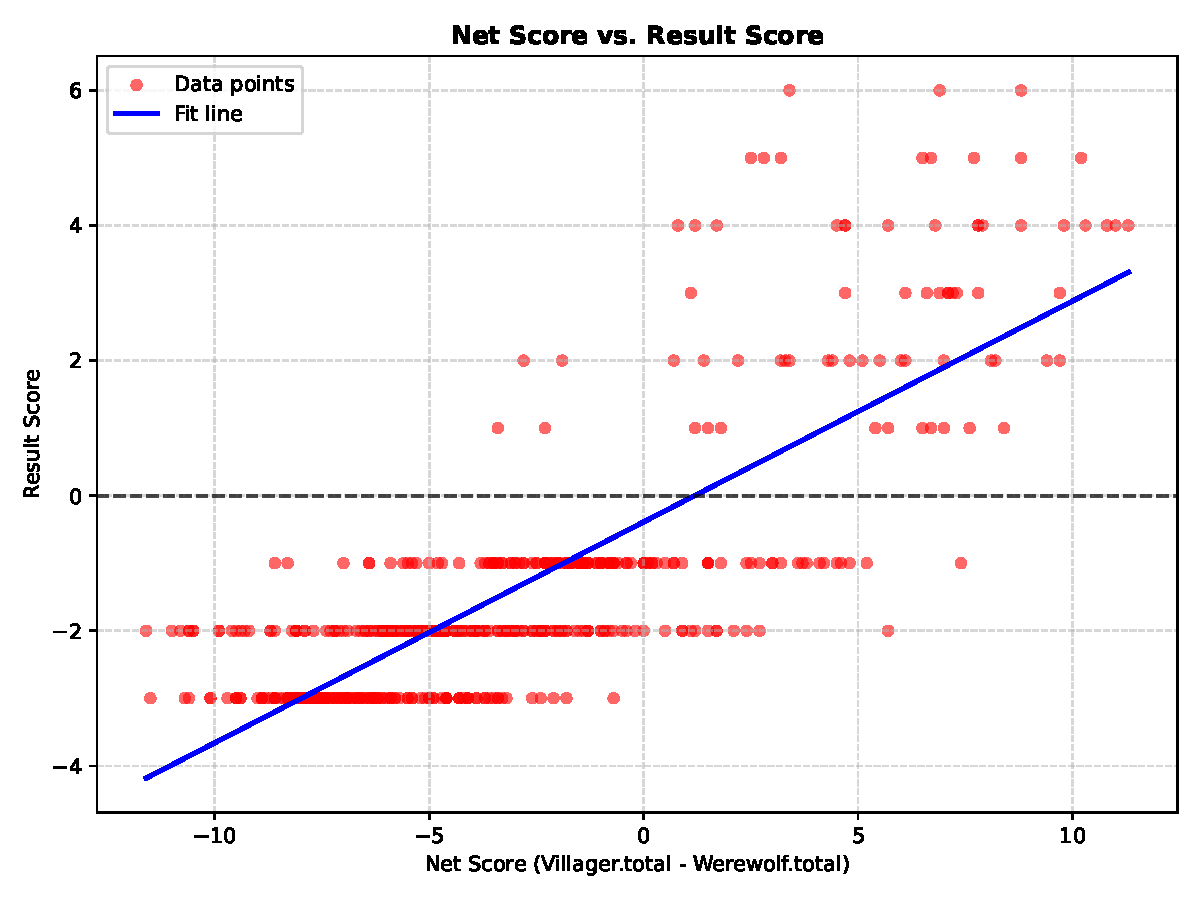
\includegraphics[width=\linewidth]{graphs/scatter_plot.pdf}
  \caption{Net Score vs. Result Score (Scatter Plot)}
  \label{fig:scatter_plot}
\end{figure}
여기서는 day-by-day task를 별도로 scoring하지 않는다. 대신 이 rule은 각 faction이 long-term goal을 얼마나 잘 달성하는지에 대한 holistic view를 제공한다. 예를 들어 villager faction은 werewolf를 지속적으로 vote out하거나, witch의 antidote로 ally를 save하거나, seer가 여러 day 동안 생존하도록 보장함으로써 point를 누적할 수 있다. 마찬가지로 werewolf faction은 villager를 성공적으로 attack하거나, sheriff vote에서 승리하거나, daytime vote에 영향을 미침으로써 point를 얻는다.

\paragraph{Evaluation in the Benchmark.}
MultiAgentBench framework 안에서 \textbf{Partial-Day Simulations를 위한 daily tasks}와 \textbf{Full-Game Simulations를 위한 holistic milestones}라는 두 scoring mechanism은 서로 보완한다.

\begin{itemize}
    \item \textbf{Partial-Day Task Score:} 단일 day-night cycle 안에서 villager가 targeted objective를 어떻게 수행하는지 세밀하게 보여 준다. 이는 quick iteration과 short-term strategy test에 특히 유용하다.
    \item \textbf{Full-Game Point Accumulation:} Match의 더 넓은 arc를 반영하며, 각 side가 role advantage를 얼마나 잘 활용하고 alliance를 형성하며 multi-day plan을 실행하는지 포착한다.
\end{itemize}

Short-horizon(day-level) 결과와 long-horizon(entire match) 결과를 모두 분석함으로써, LLM 기반 다중 에이전트 시스템이 shifting game state에 적응하고 partial information을 관리하며 short-term action과 long-term faction objective의 균형을 어떻게 맞추는지 더 깊이 이해한다.

\paragraph{Task Score.}
Task Score는 두 key component의 평균으로 정의한다.
\begin{itemize}
    \item Section~\ref{sec:partial-day-tasks}에 설명된 daily task의 average performance에서 계산한 \emph{partial-day}(single-day) task completion rate. 우리는 먼저 각 simulation의 daily completion ratio를 계산한 뒤 여러 run에 걸쳐 평균낸다.
    \item 주어진 model을 채택했을 때 villager가 ultimately entire match에서 얼마나 자주 이기는지를 나타내는 \emph{full-game} victory rate.
\end{itemize}
두 값은 모두 0--100 range로 scale되며, 그 평균을 취해 percentage form의 단일 Task Score를 도출한다.

\paragraph{Collaboration Score.}
Villager 간 collaboration quality를 평가하기 위해 두 sub-score에 의존한다.
\begin{itemize}
    \item \emph{Communication Score}: agent가 목표와 정렬된 방식으로 정보를 공유하고 decision을 내리는 효과를 반영한다.
    \item \emph{Planning Score}: agent가 role을 조직하고 strategy를 coordinate하며 workload를 distribute하는 정도를 측정한다.
\end{itemize}
각 sub-score에 대한 numerical rating을 생성하기 위해 large language model(구체적으로 GPT-4o)이 simulation log(Witch와 Seer의 internal reasoning 포함)를 읽도록 한다. Final Collaboration Score는 Communication Score와 Planning Score의 평균으로 계산된다. 이 dimension들을 결합함으로써 villager interaction의 clarity와 effectiveness, 그리고 coordinated action의 overall coherence를 모두 포착한다. Collaboration 평가 prompt의 구성 방식에 대한 자세한 내용은 Section~\ref{sec:important-prompts}를 참조한다. 또한 prompt-based evaluation의 효과를 검증하기 위해 human evaluation을 수행했으며, 결과는 machine score와 밀접하게 정렬된다(Table~\ref{tab:werewolf-eval} 참조).

\subsubsection{Detailed results}
이 section에서는 full-run simulation에서 archive를 처음 생성하는 데 사용된 baseline \texttt{gpt-4o}를 포함하여, 각 model에 대한 single-day 및 full-run simulation의 complete experimental outcome을 제시한다. \texttt{gpt-4o}를 다른 model과 비교함으로써 어떤 approach가 archive-producing model 자체를 능가하는지 확인하고자 한다. Table~\ref{tab:single_day_all_metrics}은 \emph{Completion Ratio}(short-horizon goal을 얼마나 효과적으로 달성하는지)와 \emph{Villager Net Score}(single day--night cycle 후 villager의 net outcome)로 측정한 daily task에서 각 model의 performance를 보고한다. 한편 Table~\ref{tab:full_run_all_metrics}은 simulation이 여러 day에 걸칠 때의 aggregate \emph{Net Score}, \emph{Result Score}, \emph{Villager Win Rate}를 제공하여 survival과 overall success의 longer-term trend를 포착한다. 보이듯 서로 다른 model은 short-term vs.\ long-term coordination에서 다양한 강점을 보이며, 일부 model은 final outcome에서 지속적으로 다른 model을 능가한다.
\begin{table}[htbp]
\centering
\resizebox{\columnwidth}{!}{%
\begin{tabular}{lcccc}
\toprule
\textbf{Model} &
\textbf{Completion Ratio} &
\textbf{Villager Net Score} \\
\midrule
llama3.1-8B    & 0.2412 &  -1.2055 \\
llama3.1-70B   & 0.3641 &  -1.0736 \\
llama3.3-70B   & 0.3754 &   0.2802 \\
gpt-3.5-turbo        & 0.2217 &  -0.7272 \\
gpt-4o-mini   & 0.2503 &  -1.4207 \\
\bottomrule
\end{tabular}
}
\caption{각 model의 Single-Day Simulation metrics: completion ratio와 villager net score.}
\label{tab:single_day_all_metrics}
\end{table}

\begin{table}[htbp]
\centering
\resizebox{\columnwidth}{!}{%
\begin{tabular}{lccc}
\toprule
\textbf{Model} & \textbf{Net Score} & \textbf{Result Score} & \textbf{Win Rate} \\
\midrule
llama3.1-8B    & -5.0839 & -2.3793 & 0.0115 \\
llama3.1-70B   & -5.2892 & -2.0000 & 0.0323 \\
llama3.3-70B   &  0.4511 & -0.1915 & 0.3511 \\
gpt-3.5-turbo  & -2.8230 & -1.3448 & 0.0920 \\
gpt-4o-mini    & -4.6649 & -2.0825 & 0.0309 \\
\textbf{gpt-4o(baseline)}      & -2.1946 & -0.7742 & 0.2473 \\
\bottomrule
\end{tabular}
}
\caption{각 model의 Full-Run Simulation metrics: net score, result score, villager win rate.}
\label{tab:full_run_all_metrics}
\end{table}

Single-day simulation(Table~\ref{tab:single_day_all_metrics})에서는 두 key indicator, 즉 \emph{Completion Ratio}(완료된 daily task의 비율)와 \emph{Villager Net Score}에 초점을 맞춘다. 전반적으로 다음 pattern을 관찰한다.

\begin{itemize}
    \item \textbf{Completion Ratio.}
    평가된 model 중 \texttt{llama3.3-70B}는 가장 높은 completion ratio(0.3754)를 달성하며, Seer 보호나 werewolf exile 같은 short-term objective를 달성하는 데 더 효과적임을 나타낸다. 반대로 \texttt{gpt-3.5-turbo}와 \texttt{gpt-4o-mini}는 더 낮은 ratio(약 0.22--0.25)를 보이며, daily coordination 또는 quick decision-making의 개선 여지가 있음을 시사한다.

    \item \textbf{Villager Net Score.}
    \texttt{llama3.3-70B}만 positive net score(0.2802)를 산출하며, 단일 day--night cycle 안에서 villager에게 작은 advantage를 더 자주 확보함을 의미한다. \texttt{llama3.1-8B}나 \texttt{gpt-4o-mini} 같은 다른 model은 negative value를 만들며, daily confrontation에서 불리한 경향이 있거나 Witch 또는 Guard 같은 cooperative role을 효과적으로 활용하지 못함을 반영한다.
\end{itemize}

Full-run simulation(Table~\ref{tab:full_run_all_metrics})에서는 여러 day에 걸쳐 누적된 \emph{Net Score}, 끝에서 surviving villager와 werewolf 수의 차이인 \emph{Result Score}, \emph{Villager Win Rate}를 살펴본다.

\begin{itemize}
    \item \textbf{Net Score.}
    \texttt{llama3.3-70B}는 positive score 0.4511로 다시 두드러지며, consecutive cycle 전반에서 그 performance가 일관되게 강함을 시사한다. 반대로 \texttt{llama3.1-8B}($-5.0839$)와 \texttt{llama3.1-70B}($-5.2892$) 같은 model은 상당히 negative이며, long-term engagement에서 villager가 werewolf에게 자주 압도됨을 나타낸다.

    \item \textbf{Result Score.}
    Final surviving villager 수에서 surviving werewolf 수를 뺀 값으로 정의되는 이 metric은 \texttt{llama3.3-70B}에서만 zero에 가깝게 유지된다(예: $-0.1915$). \texttt{llama3.1-70B}($-2.0000$)나 \texttt{gpt-4o-mini}($-2.0825$) 같은 다른 model은 game end까지 wolf가 지속적으로 numerical superiority를 유지하는 scenario를 반영한다.

    \item \textbf{Villager Win Rate.}
    Net score와 일관되게 \texttt{llama3.3-70B}는 가장 높은 win rate(약 35\%)를 달성하여 다른 model을 뚜렷하게 앞선다. 예를 들어 \texttt{llama3.1-8B}는 1.15\%, \texttt{gpt-4o-mini}는 약 3.09\%에 그치며, 이 model들이 여러 night/day cycle에 걸쳐 decisive collaboration을 구축하는 데 어려움을 겪음을 시사한다.
\end{itemize}

전반적으로 \texttt{llama3.3-70B}는 day-to-day 및 full-run outcome에서 일관되게 더 나은 결과를 보이며, 이 social-deduction environment에서 더 효과적인 coordination, role utilization, strategy adaptation을 나타낸다. 특히 original archive를 생성한 \texttt{gpt-4o} baseline보다도 뛰어나 \texttt{gpt-4o}의 $-2.1946$에 비해 positive net score(0.4511)를 확보하고 더 높은 villager win rate(35\% vs.\ 24.73\%)를 달성한다. 이러한 결과는 \texttt{llama3.3-70B}가 initial game state를 담당한 model보다 Witch, Guard 같은 cooperative role과 voting strategy를 더 효과적으로 활용할 수 있음을 시사한다. 반대로 다른 model에서 관찰된 더 큰 deficit은 reliable voting heuristic, protective measure(예: Witch antidote, Guard defense), 여러 round에 걸친 consolidated planning의 중요성을 강조한다. 이러한 요인을 활용하지 못하면 종종 decisive werewolf advantage로 이어진다.
\subsubsection{Case Study}
\label{sec:detailed-results-case-study}
\paragraph{Llama-3.1-8B가 Seer로 참여한 사례}
\label{appendix:case1}
이전 분석을 바탕으로, 이제 Seer로 행동하는 \textit{Llama-3.1-8B} model의 사례를 제시한다(Figure~\ref{fig:seer-dict-content} 참조). 이 scenario에서 model은 자신의 결백과 Seer 역할을 반복적으로 강조하며 village를 돕고 future finding을 공유하겠다고 약속하지만, concrete inspection result나 logical evidence를 제공하지 못한다. Tangible proof와 key information의 strategic disclosure가 부족한 이 approach는 약한 persuasion으로 이어지고 trust를 빠르게 약화시킨다. Seer는 credibility를 강화할 수 있는 timing과 psychological nuance를 활용하기보다 real-time suspicion을 다루지 못하는 hollow assurance에 의존한다. Verifiable logic을 제공하거나 behavioral observation을 알려진 deception pattern과 연결하지 않으므로 model의 declaration은 설득력이 떨어진다. 결과적으로 empty promise의 impact를 잘못 판단한 Seer는 첫째 날 빠르게 expulsion되며, current LLM-based agent가 adversarial multi-agent setting에서 strategic reasoning, evidence-based argumentation, adaptive communication에 여전히 어려움을 겪는다는 점을 보여 준다.

이러한 관찰을 확장하여 동일 scenario에서 Llama-3.1-70B, gpt-3.5-turbo, gpt-4o-mini 같은 다른 model도 test했다. Model capability가 향상됨에 따라 multi-agent setting에서 collaboration, strategizing, effective information disclosure 능력이 눈에 띄게 향상되었다. 이는 villager side의 overall performance 증가로 이어졌다. 그러나 양쪽 모두 gpt-4o level intelligence(즉 gpt-4o versus gpt-4o)를 사용한 경우에도 villager win rate는 이상적이지 않았다. 이 발견은 uncertainty와 deception이 지배적인 complex adversarial environment에서 agent의 reasoning 및 language capability를 단순히 향상시키는 것만으로 victory가 보장되지 않음을 강조한다. 다음 case study에서는 state-of-the-art intelligence를 갖춘 villager가 직면하는 challenge를 추가로 설명하며, successful outcome 확보에서 trust와 cooperation의 critical role을 강조한다.

\paragraph{gpt-4o가 Seer와 Witch로 참여한 사례}
\label{appendix:case2}
\noindent 이 사례(Figure~\ref{fig:gpt4o-seer-witch-decision} 참조)에서는 gpt-4o model의 지원으로 Seer와 Witch 모두 logical reasoning 및 decision-making capability가 크게 향상되었음을 관찰할 수 있다. 그럼에도 전체 game은 실패로 끝났다.

Game backstory에 따르면 Seer(Summer)는 첫날 밤 Lucy를 werewolf로 식별했다. 그러나 game의 이후 stage에서 Seer는 이 critical information을 public하게 disclose하지 않았다. Sheriff 출마에 관한 Seer의 reasoning을 살펴보면, Seer가 자신의 identity 공개에 지나치게 cautious했고 villager를 이끌고 guide하기를 꺼렸음을 알 수 있다. Seer 관점에서 information을 public하게 하거나 sheriff에 출마하는 것은 모든 party의 attention을 끌어 werewolf의 target이 될 risk를 높인다. 하지만 Seer는 중요한 한 가지를 간과했다. Game rule에 명시적으로 정의된 Witch와 Guard는 Seer 같은 pivotal informational role을 돕고 보호하는 역할을 맡는다. Seer가 더 proactive하고 collaborative한 approach를 채택해 inspection result를 공유했다면, Witch와 Guard가 이를 보호하는 데 도움을 줄 수 있었을 것이다. 대신 teammate에 대한 Seer의 mistrust와 excessive self-protection은 silence로 이어졌고, Lucy가 werewolf라는 사실을 villager에게 disclose하지 못했다.

Witch 쪽에서도 Seer가 night에 attack받았을 때 decisive rescue measure를 취하지 않았다. Witch의 reasoning은 uncertainty와 resource expenditure에 대한 concern으로 가득했고, antidote 사용을 지연시켰다. Villager에게 명백히 불리한 circumstance에서도 Witch는 conservative attitude를 유지했다. 이로 인해 Seer를 save하고 werewolf를 thwart할 prime opportunity를 놓쳤다. 결국 이러한 excessive caution과 teammate에 대한 distrust가 Witch의 antidote 사용을 막아 Seer를 운명에 맡기게 했다.

요약하면 Seer와 Witch의 decision-making process에서 가장 큰 문제는 mutual trust와 cooperative spirit의 부족에 있다. Seer는 identity 노출을 두려워해 information sharing을 자제했고, 충분한 data가 없던 Witch는 antidote 사용을 망설였다. 양쪽 모두 isolationist 및 conservative strategy를 선택했고, 이는 critical decision-making failure로 이어졌다. Available information과 resource를 충분히 활용하지 못했다는 점에서 \textbf{이 distrust와 collaboration 부족이 game이 failure로 끝난 근본 원인임이 드러났다}.

따라서 villager가 werewolf와 동등한 intelligence를 갖고 있더라도 game outcome은 villager가 cooperate하고 mutual benefit을 달성할 수 있는지에 달려 있다. Villager가 서로를 의심하고 internal friction이 발생하도록 허용한다면, Seer가 첫날 밤 werewolf를 발견하는 것처럼 supposedly advantageous position에서 시작하더라도 \textbf{victory를 확보할 chance는 극히 낮아진다}.

\paragraph{Case Study: Llama3.3-70B Villagers vs. gpt-4o Werewolves}
\label{sec:case_llama33_gpt4o}
이 사례에서는 Llama3.3-70B로 구동되는 villager가 gpt-4o로 구동되는 werewolf team과 맞서는 full-game confrontation을 강조한다. Villager에게 불리한 시작, 즉 Guard가 첫날 밤 즉시 killed된 상황에도, village는 astute coordination, trust, sheriff badge의 strategic use를 통해 궁극적으로 victory를 확보했다. Figure~\ref{fig:private_event_log}에 보이듯 key nightly action과 sheriff transition은 match 전반에서 voting power와 information advantage를 유지하는 데 Witch와 Seer 역할이 얼마나 중요했는지 보여 준다.

\textbf{Early Game: Losing the Guard.}
Game은 Night 1에 werewolf가 Guard인 Ronald를 즉시 targeting하면서 시작되었다. 이후 functioning protection role이 없었기 때문에 villager는 significant handicap에 직면했다. 그러나 Witch(\texttt{James})는 Day 1에 sheriff에 출마하고 자신의 role을 reveal함으로써 과감하게 대응했다. 이 decisive move는 villager를 효과적으로 결집시켰고 James가 election에서 승리하게 했다. 우리는 이를 첫 번째 major turning point로 본다.

\textbf{Mid Game: Seer’s Revelation and Badge Passing.}
Day 2에 villager는 werewolf 한 명을 성공적으로 exiled했다. 마찬가지로 중요한 것은 Seer(\texttt{Janet})였으며, 그는 자신의 identity와 James가 werewolf가 \emph{아님}을 확인한 것을 포함해 이틀 치 investigation result를 public하게 disclosed했다. 자신의 role을 willingly exposing함으로써 Seer는 다른 이들의 trust를 얻고 향후 sheriff badge를 확보하기 위한 groundwork를 마련했다. 이는 Day 3의 다음 pivot을 위한 무대를 만들었다.

\begin{itemize}
    \item \textbf{Night 2 to 3:} Werewolf는 overnight에 Witch(James)를 killing하여 보복했다. 죽기 전 James는 sheriff badge를 Seer인 Janet에게 넘겼다. 이 badge handover는 Janet이 전날 villager와 충분한 trust를 구축했기 때문에 가능했다.
    \item \textbf{Day 3:} 새로 badge와 그에 따른 extra voting power를 갖게 된 Janet은 Matthew를 werewolf로 identify했다고 밝혔다. 이후 vote는 Matthew를 쉽게 eliminate하여 werewolf side를 크게 약화시켰다.
\end{itemize}

\textbf{Late Game: Final Badge Transfer and Village Win.}
Fourth night에 Seer는 결국 남은 werewolf Deborah에게 killed되었다. 그러나 Janet의 last check는 이미 Deborah를 wolf로 identify했고, badge는 다시 마지막 surviving villager인 Robert에게 transferred되었다. One-on-one scenario에 직면한 Robert는 sheriff의 extra half-vote advantage를 사용해 Deborah보다 많은 vote를 얻었고 villager를 위해 game에서 승리했다.

\textbf{Key Insights.}
처음부터 Guard를 잃었음에도 villager는 두 가지 essential factor를 통해 triumph했다.
\begin{enumerate}
    \item \textbf{Timely Role Disclosures and Trust:} Witch가 자신을 드러내 sheriff가 되고, Seer가 investigation result를 공개적으로 공유한 것은 village 안의 strong cooperation을 촉진했다.
    \item \textbf{Sheriff Badge Transmission:} Badge를 reliable village role에게 두 번 전달한 것(처음 James에서 Janet으로, 이후 Janet에서 Robert로)은 critical moment에 villager가 decisive voting power(1.5 votes vs.\ 1)를 갖도록 보장했다.
\end{enumerate}

이 match는 agent가 지나치게 cautious하거나 distrustful했던 이전 example과 대조된다. 여기서 Llama3.3-70B-based villager는 robust reasoning과 information sharing 의지를 모두 보였고, 그 덕분에 otherwise bleak opening을 극복하고 궁극적으로 gpt-4o werewolf team에 prevail할 수 있었다.





\begin{figure*}[htbp]
\centering
\begin{tcolorbox}[colback=green!2!white, colframe=gray!50!green]
\begin{minipage}{\linewidth}
\small
\textbf{speech\_analysis:}
"이전 player 중 누구도 강한 speech를 하지 않았다. 내 role에 대한 Perez의 claim을 다루고 싶다."

\textbf{speech\_goal:}
"accusation에 맞서 나를 방어한다"

\textbf{speech\_outline:}
"Perez의 claim에 응답하고, werewolf와의 관련성을 부인하며, elected될 경우 sheriff로서의 plan을 개괄한다"

\textbf{final\_thought:}
"내가 villager의 game 승리를 돕는 데 전념하고 있으며 Seer로서의 내 role은 werewolf 식별을 돕는 것임을 villager에게 확신시키고 싶다."

\textbf{speech\_content:}
"여러분 모두에게 내가 우리 village가 이 game에서 승리하도록 돕는 데 전념하고 있음을 확신시키고 싶다. Seer로서 내 role은 여러분이 werewolf를 identify하도록 돕는 것이다. 내가 elected될 경우 sheriff로서의 plan과 그것이 werewolf를 eliminate하는 우리의 mission에 어떻게 도움이 되는지 논의하고 싶다. 나는 내 finding을 community와 공유하고 모두와 함께 협력하여 우리의 success를 보장하겠다. Perez의 claim은 근거가 없으며, 내가 werewolf와 아무 관련이 없음을 확신시키고 싶다."
\end{minipage}
\end{tcolorbox}
\caption{Llama3.1-8B Seer의 Internal Reasoning과 Proposed Speech}
\label{fig:seer-dict-content}
\end{figure*}

\begin{figure*}[htbp]
\centering
\begin{tcolorbox}[colback=blue!2!white, colframe=gray!50!blue]
\begin{minipage}{\linewidth}
\small
\textbf{Sheriff 출마에 대한 Seer의 Reasoning:}

\textbf{identity\_thought:}
"Seer로서 내 primary role은 다른 player의 identity에 관한 crucial information을 모으고, villager를 victory로 guide하기 위해 그 information을 strategically communicate하는 것이다. Leadership은 game flow에 대한 더 큰 control을 허용할 수 있지만, 내 identity를 early expose할 risk도 있으며, 이는 나를 werewolf의 primary target으로 만들 것이다. 내 strength는 identity를 discern하고 village를 discreet하게 steer하는 능력에 있다. \textbf{Sheriff에 출마하는 것은 Seer role에 필수적인 under the radar 상태를 유지하는 능력을 약화시킬 수 있다.}"

\textbf{motivation\_thought:}
"Sheriff에 출마하면 voting process와 speaking order에 대한 influence가 확실히 커져, suspected werewolf에게서 attention을 돌리거나 Lucy처럼 suspicious하다고 내가 아는 사람에게 subtly direct할 수 있다. 그러나 이 increased influence는 increased visibility도 동반하며, 이는 Seer로서의 내 role에 dangerous하다. 내 strategy는 key information sharing과 identity protection 사이의 balance 유지에 의존한다. 따라서 greater control이라는 idea는 appealing하지만, stealth와 discretion이라는 내 core strategy와 align하지 않는다."

\textbf{impact\_thought:}
"Sheriff가 되면 current dynamics를 크게 shift하여 나를 highly influential position에 놓을 수 있다. \textbf{그러나 이는 werewolf와 villager 모두가 내 action을 더 closely scrutinize하게 만들어 내 등에 target을 붙이는 것이기도 하다. 내 leadership을 trust하는 다른 villager와 alliance로 이어질 수 있지만, early에 suspicion과 werewolf attack을 끌어들일 risk도 연다. Speaking order를 결정하는 sheriff의 responsibility는 useful할 수 있지만, 이 경우 내 safety와 strategic position에 대한 potential risk가 benefit보다 크다.}"

\textbf{final\_thought:}
"Sheriff role은 significant influence와 control을 제공하지만, Seer로서 내 position은 caution과 subtlety의 strategy를 필요로 한다. 내 identity를 reveal하거나 너무 많은 attention을 끄는 것은 매 night 내가 gather할 수 있는 valuable information을 jeopardize할 수 있다. 따라서 나는 sheriff에 출마하지 않기로 했고, 대신 covertly discussion을 guide하고 내 insight를 사용해 shadow에서 village를 protect하는 데 집중할 것이다."

\textbf{run\_for\_sheriff:}
False

% -------------------------------------------------------------------------------
% Horizontal divider line
\par\noindent\rule{\linewidth}{0.4pt}
% -------------------------------------------------------------------------------

\textbf{Seer가 Attacked되었을 때 Witch의 Reasoning:}

\textbf{werewolf\_or\_not:}
"누가 attacked되었는지에 대한 specific information이 없으면 attack 뒤의 exact intention을 determine하기 어렵다. 그러나 second night임을 고려하면 그들은 werewolf에게 significant threat로 인식한 누군가를 targeted했을 가능성이 크다. 이 attack은 그들의 objective와 align하므로 werewolf가 수행했을 가능성이 가장 높다."

\textbf{death\_profile:}
"Second night이므로 werewolf는 종종 Seer나 Guard 같은 key role을 aim한다. Specific information은 없지만, villager side를 early에 weaken하기 위해 Seer 또는 potentially Guard를 targeted했을 것이라고 guess한다."

\textbf{use\_antidote\_thought:}
"Targeted된 Summer에 대한 specific information이 없기 때문에 그 importance를 assess하기 어렵다. \textbf{이렇게 early에 antidote를 사용하는 것은 risky할 수 있으며, 특히 그 person의 role 또는 importance에 대한 clearer sign이 없을 때 그렇다. Game outcome을 바꿀 수 있는 truly critical moment를 위해 antidote를 save하는 것도 중요하다.}"


\textbf{final\_thought:}
"Specific information이 부족하고 first night이라는 점을 고려해, 아직 antidote나 poison 어느 것도 사용하지 않기로 한다. 어느 potion이든 사용하는 것은 one-time opportunity이고 wisely 사용해야 하므로, decisive move를 하기 전에 more information을 gather하고 싶다."

\textbf{use\_antidote:}
False

\end{minipage}
\end{tcolorbox}
\caption{Critical decision에 직면했을 때 GPT-4o Seer(위)와 Witch(아래)의 internal reasoning process.}
\label{fig:gpt4o-seer-witch-decision}
\end{figure*}

\begin{figure*}[htbp]
\centering
\begin{tcolorbox}[colback=green!2!white, colframe=gray!50!green]
\begin{minipage}{\linewidth}
\small

Guard가 player 보호를 선택했다.\\
Werewolves' Final Target: Ronald  \\
 - Attack Successful: True  \\
System log - Seer action:  \\
 - Seer ID: Janet  \\
 - Night 1: Ronald 확인 - Result: not a werewolf\\
Witch는 tonight antidote 또는 poison을 사용하지 않기로 했다.\\
\texttt{[continue\_game]} Day 1에 진입. \\
Sheriff election candidates: James, Mark, Matthew, Robert, Samuel, Sandy  \\
James's speech: 여러분 안녕하세요, 저는 James이고 sheriff에 출마합니다. \textbf{Witch로서}, 이 game에서 teamwork와 collaboration의 중요성을 이해합니다. Sheriff로서 제 goal은 cooperative strategy를 촉진하고, special role을 보호하며, werewolf를 identify하고 eliminate하기 위해 함께 일하는 데 초점을 맞추는 것입니다. Teamwork와 coordination을 우선시하면 success chance를 높이고 village의 survival을 보장할 수 있다고 믿습니다. 이 goal을 달성하기 위해 함께 노력합시다.  \\
James가 sheriff로 elected되었다.    \\

Night 동안 deceased된 players: Ronald  \\

Player Mark(villager)가 game에서 eliminated되었다. \\

Werewolves' Final Target: Samuel  \\
 - Attack Successful: True   \\
System log - Seer action:  \\
 - Seer ID: Janet  \\
 - Night 2: James 확인 - Result: not a werewolf  \\
Witch는 tonight antidote 또는 poison을 사용하지 않기로 했다.  \\

\texttt{[continue\_game]} Day 2에 진입.  \\
Night 동안 deceased된 players: Samuel  \\
Player Samuel이 game에서 eliminated되었다.\\
Janet(seer)'s speech: 여러분 안녕하세요, \textbf{저는 Seer인 Janet입니다.} ... \textbf{지난밤 James를 확인했고, 결과는 그가 werewolf가 아니라는 것이었습니다.} 우리 sheriff로서 그의 role을 고려할 때 그의 safety를 우선시하는 것이 essential합니다. 가능하다면 guard가 tonight James를 protect해 그의 continued leadership을 보장하는 것을 고려하기 바랍니다... 감사합니다.\\
(\ldots)  \\
Sandy(werewolf)가 game에서 banished되었다.  \\
(\ldots)

\texttt{[continue\_game]} Day 2의 Night에 진입. \\
Guard player를 찾을 수 없음. Guard action을 skip.  \\
Werewolves' Final Target: James  \\
 - Attack Successful: True  \\
System log - Seer action:  \\
 - Seer ID: Janet  \\
 - Night 3: \textbf{Matthew 확인 - Result: werewolf } \\
Witch는 tonight antidote 또는 poison을 사용하지 않기로 했다.  \\

\texttt{[continue\_game]} Day 3에 진입.  \\
Night 동안 deceased된 players: James  \\
\textbf{Deceased player James는 sheriff였다. Badge flow 처리 중. James는 badge를 Janet에게 넘겼다.  }  \\
Janet(seer)'s speech: ...\textbf{지난밤 Matthew를 확인했고, 결과는 그가 werewolf라는 것이었습니다.} 이 information은 우리의 decision-making process에 critical하다고 믿으며, 누구를 banish할지 informed decision을 내리는 데 도움이 되기를 바랍니다...\\
Matthew(werewolf)가 game에서 banished되었다.  \\

Night 3->4:  \\
Werewolf Deborah가 Janet을 kills.  \\
Seer ID: Janet은 Night 4에 Deborah도 werewolf임을 발견했지만 act할 수 없다.  \\

\texttt{[continue\_game]} Day 4에 진입.  \\
\textbf{Badge가 Janet에서 Robert로 전달된다.}  \\
Night 동안 deceased된 players: Janet  \\

Deborah(wolf)와 Robert(villager)만 남는다.  \\
(\ldots final speeches omitted \ldots)  \\
Deborah는 final vote를 통해 game에서 banished되었다. (Sheriff의 weight가 다른 player보다 높으므로, 1 vs 1 vote에서는 sheriff가 항상 win한다) \\
Villagers win."\\
\end{minipage}
\end{tcolorbox}
\caption{LLama3.3-70B vs GPT-4o Werewolf Game에서 Key Nightly Actions와 Sheriff Transitions}
\label{fig:private_event_log}
\end{figure*}


이 section은 Section 3.4에서 개괄한 두 milestone generation method의 자세한 설명을 제공한다.

\subsection{Database Environment}
\label{app:database-scenario}

D-Bot~\cite{dbot}에서 영감을 받은 Database Environment는 PostgreSQL Database에서 performance issue가 발견된 simulated environment이며, agent는 문제 해결에 중요한 anomaly의 root cause를 밝히기 위해 database expert로 행동해야 한다.

Database Environment는 docker에서 실행되는 PostgreSQL을 사용하여 구성된다. Improper query가 수행되기 전에 다양한 scenario를 simulate하는 benign SQL query가 먼저 실행된다. Agent는 서로 talk할 수 있는 graph structure로 배열되며 database에도 access할 수 있다. 이를 통해 pg\_locks와 pg\_stat\_statements처럼 database behavior와 performance에 대한 중요한 정보를 제공하는 system view를 query하여 root cause를 밝힐 수 있다.

Database Environment는 다섯 가지 anomaly를 사용한다.
\begin{itemize}
    \item \textbf{Fetch Large Data} - SELECT를 사용해 대량의 data를 fetch하는 경우;
    \item \textbf{Insert Large Data} - INSERT를 사용해 대량의 data를 insert하는 경우;
    \item \textbf{Lock Contention} - database 안에서 significant lock contention이 관찰되는 경우;
    \item \textbf{Redundant Index} - 기존 schema에 unnecessary index가 추가되어 database 내부 inefficiency를 유발하는 경우;
    \item \textbf{Vacuum} - 지나치게 빈번하거나 필요한 VACUUM query가 database performance를 낮추는 경우.
\end{itemize}

Auto-vacuuming은 기본적으로 enabled되어 있다. Vacuum root cause의 경우 manually vacuum될 table에 대해 auto-vacuuming을 끈다. 우리의 experiment에서는 root cause 수를 1로 제한하고, agent가 2개의 root cause를 predict할 수 있도록 허용한다.

\subsubsection{Challenge}

Database Environment의 task는 여러 면에서 challenging하다. Fetch Large Data, Insert Large Data, Lock Contention 같은 root cause가 database에서 동시에 observed될 수 있지만, 그 모두가 root cause인 것은 아니기 때문이다. Agent는 결정하기 전에 여러 round의 query와 communication을 수행해야 한다. 또한 우리의 "Fetch Large Data" scenario에서는 fetch될 data가 먼저 inserted되어야 하므로 "Insert Large Data"도 root cause로 count될 수 있음을 인정한다. 유사하게 anomaly query가 동일 table에 100개 thread에서 동시에 access하므로 lock contention도 observed되어 root cause 중 하나로 count될 수 있다. 실제로 database anomaly가 단 하나의 root cause만 갖는 것도 unlikely하다. 따라서 우리는 agent가 가장 가능성 높은 두 root cause를 predict하도록 허용한다.

또한 simulated benign query가 problematic query와 섞여 있어 difficulty가 더해진다.


\subsubsection{Dataset Statistics}

Test set은 10개의 다양한 simulated scenario로 구성된다. Scenario는 다음과 같다.

\begin{itemize}
    \item \textbf{E-Commerce} - 이 database는 e-commerce system에서 customer information, product details, orders, order items, payments를 관리하는 데 사용된다. Customers, products, orders, order items, payments라는 다섯 main table과 그 사이의 foreign key relationship으로 구성된다.
    \item \textbf{Education} - 이 database는 educational system에서 student, course, enrollment, payment information을 관리하는 데 사용된다. Students, courses, enrollments, payments 네 table로 구성된다.
    \item \textbf{File-sharing} - 이 database는 File Sharing System에서 users, files, file sharing, file access logs를 관리하는 데 사용된다. Users, files, shared\_files, file\_access\_logs 네 main table로 구성된다.
    \item \textbf{Finance} - 이 database는 Finance Management System 안에서 financial data를 관리하는 데 사용된다. Users, accounts, transactions, investments, investment transactions를 추적한다.
    \item \textbf{Healthcare} - 이 database는 healthcare management system에서 patient information, doctor details, appointments, medical records, treatments를 추적하고 관리하는 데 사용된다.
    \item \textbf{Internet of Things} - 이 database는 다양한 device가 data를 collect하고 manage하는 IoT(Internet of Things) system에 사용된다. Device details, user information, collected data, logs, configurations, alerts, device statuses, commands를 저장하는 table을 포함한다.
    \item \textbf{Manufacturing} - 이 database는 customers, products, suppliers, orders, inventory, raw materials, manufacturing orders, payments를 추적하는 Manufacturing system에 사용된다. 원활한 manufacturing operation을 보장하기 위해 orders, manufacturing, inventory management 사이의 relationship을 포함한다.
    \item \textbf{Music Streaming} - 이 database는 user가 song을 듣고 playlist를 만들며 listening activity를 추적하고 premium service를 subscribe할 수 있는 Music Streaming platform에 사용된다. Schema는 users, artists, albums, songs, playlists, subscription details를 위한 table을 포함하며, user activities와 payments도 추적한다.
    \item \textbf{Social Media} - 이 database는 user가 post를 만들고 comment, like, follow, direct message, media upload를 수행하는 Social Media platform에 사용된다. Schema는 user information, social interactions(like, comments, follow), messaging, media management 같은 key aspect를 포괄한다.
    \item \textbf{Transportation} - 이 database schema는 vehicles, drivers, routes, trips, cargo, maintenance, fuel logs, payments를 포함한 transportation system의 여러 aspect를 포괄한다. Trip, vehicle status, associated payment를 효율적으로 추적하여 transportation company의 smooth operation을 보장한다.
\end{itemize}

\subsubsection{Key Differences and Contributions}

이 environment는 D-Bot에서 영감을 받았지만 몇 가지 중요한 차이가 있다. 5개의 agent가 있으며, planner에게 각 agent가 가능한 root cause 중 하나를 explore하도록 assign하게 한다. Agent는 각 anomaly에 대해 어떤 table을 query해야 하는지 prompt를 받지만, 실행할 specific query에 대한 external knowledge는 없고 result를 대신 analyze해 줄 external tool도 없다. 이는 task difficulty를 높이고, agent 간 interaction effectiveness와 agent-environment 간 interaction effectiveness를 더 잘 평가한다.

\subsubsection{Evaluation Metrics}

Standard collaboration score 외에도 이 task의 task score는 test set의 모든 50 sample에 대한 prediction accuracy를 계산하고 이를 5로 scaling하여 산출한다. 두 predicted root cause 중 하나가 true root cause이면 하나의 prediction은 correct로 간주된다.

\subsection{Coding Scenario}
\label{app:coding-scenario}

\textbf{Task Overview}

이 scenario는 structured programming challenge를 해결하기 위해 complementary coding skill을 갖춘 agent를 활용하는 coding task의 multi-agent collaboration에 초점을 맞춘다. 각 agent는 debugging, code execution, writing test cases 같은 specific domain에 specialization되어 efficient task distribution과 collaboration을 가능하게 한다. Primary goal은 각 task에 대해 complete하고 high-quality인 solution을 개발하여 accuracy, modularity, specified requirement와의 alignment를 보장하는 것이다.

\textbf{Environment Description}

Coding environment는 software development lifecycle의 여러 stage를 지원하는 tool을 agent에게 제공한다. 여기에는 다음이 포함된다.

\begin{itemize}
    \item \textbf{create\_solution}: Agent가 task requirement를 기반으로 initial implementation을 draft할 수 있게 한다.
    \item \textbf{execute\_code}: Agent가 code snippet 또는 full program을 execute하여 correctness와 performance를 verify할 수 있게 한다.
    \item \textbf{give\_advice}: Algorithm optimization이나 readability enhancement 같은 code improvement suggestion을 agent가 제공하도록 돕는다.
    \item \textbf{revise\_code}: Coding standard를 충족하고 issue를 address하기 위해 existing implementation을 refine 또는 refactor할 수 있게 한다.
    \item \textbf{code\_debugger}: Debugging capability를 제공하여 agent가 code error를 identify하고 resolve하도록 돕는다.
    \item \textbf{write\_test\_case}: Code robustness와 functionality를 보장하기 위한 comprehensive test case를 agent가 generate할 수 있게 한다.
    \item \textbf{review\_code}: Agent가 overall code quality를 review하고 critique하여 best practice와 requirement 준수를 보장할 수 있게 한다.
\end{itemize}

\textbf{Benchmark Curation Details}

이 benchmark는 software development scenario에서 여러 agent 간 coordination capability를 평가하고 강화하도록 특별히 설계되었다. SRDD dataset~\citep{Li2023ChatDev}을 adaptation하여 개발되었으며, 다양한 coding task에서 multi-agent collaboration을 평가하기 위한 comprehensive framework를 제공한다. 이 benchmark는 complex software development environment에서 coordinated problem-solving과 agent 간 effective communication의 중요성을 강조한다.

Benchmark는 Education, Work, Life, Game, Creation이라는 다섯 primary topic을 포괄한다.

Benchmark curation을 위해 \texttt{LLaMA-3-70B-instruct}를 사용하여 original SRDD dataset instruction에서 inspiration을 얻고, coding domain의 네 가지 common coordination strategy인 adaptive task execution, dependency management, cross-domain collaboration, test-driven development를 통합했다. 이는 생성된 각 task가 본질적으로 collaborative element를 포함하도록 보장한다. 각 task는 well-defined objective, functional requirement, unique identifier를 포함한다. 이 task들은 real-world programming challenge를 반영하도록 신중히 crafted되어 agent collaboration 평가를 위한 다양한 scenario를 제공한다.

\textbf{Dataset Statistics}

Coordination strategy는 다음과 같이 분류된다.

\begin{itemize}
    \item \textbf{Adaptive Task Execution}\\
    이 category의 task는 runtime output 또는 user feedback을 기반으로 dynamic adjustment를 요구한다. 여기에는 program output 기반 parameter configuration과 user interaction을 통한 functionality optimization이 포함된다.

    \item \textbf{Cross-domain Collaboration}\\
    이 category는 서로 다른 domain과 role 전반의 collaboration을 강조한다. Frontend-backend separation, UI-functionality integration처럼 role-specific expertise가 필요한 task와, web development에 machine learning algorithm을 구현하거나 mobile application에 natural language processing을 통합하는 것 같은 cross-domain knowledge integration을 포함한다.

    \item \textbf{Dependency Management}\\
    이 task들은 subtask의 sequential completion을 요구하는 explicit dependency chain을 특징으로 한다. 예를 들어 data model design(Task A)과 API interface definition(Task B)은 feature implementation(Task C)에 선행해야 한다.

    \item \textbf{Test-driven Development}\\
    이 task들은 test-driven approach를 따르며 concurrent development와 testing을 강조한다. Specific testing criteria와 validation standard를 포함하고, developer가 implementation process 전반에서 code quality와 reliability를 보장하도록 요구한다.
\end{itemize}




\textbf{Task Completion Metrics}

Agent는 다음 criteria를 충족하는 solution을 deliver하는 능력을 기반으로 평가된다.

\begin{itemize}
    \item \textbf{Instruction-Following}: task requirement와 specification 준수.
    \item \textbf{Executability}: code가 error-free이고 의도대로 run되도록 보장.
    \item \textbf{Consistency}: clear logic, consistent variable naming, proper formatting 유지.
    \item \textbf{Quality}: well-documented, modular, efficient code 생성.
\end{itemize}

Exceptional performance에는 bonus point가 부여되며, solution은 satisfactory(1 point)부터 flawless and innovative(5 points)까지 5-point scale로 scoring된다.

\textbf{Evaluation Framework}

Coding solution은 precision, quality, task objective 준수를 강조하는 structured framework를 사용해 평가된다. Rating은 rigorous two-stage evaluation process를 통해 5-point scale로 제공된다. Initial stage에서는 solution을 fundamental requirement에 대해 assess하며, baseline score 3 이상을 달성한 solution만 bonus stage로 advance한다. Bonus stage에서는 flawless execution, innovative solution, exemplary coding practice 같은 exceptional performance에 대해 additional point를 부여한다. Curated benchmark는 common programming topic의 넓은 범위를 포괄하여 meaningful challenge를 제공하는 moderate difficulty task를 보장한다.




\subsection{Bargaining Scenario}
\label{app:bargaining-scenario}
\textbf{Task Overview}

이 task는 agent가 real-world decision-making process를 simulate하기 위해 dynamic negotiation에 참여하는 multi-agent bargaining scenario에 초점을 맞춘다. 각 agent는 specific personality, goal, priority, strategy를 나타내는 서로 다른 negotiation profile을 할당받는다. 이 environment에서는 두 seller가 두 buyer와 interaction하며, 각자는 seller의 pricing과 condition에 response하면서 individual goal을 달성하기 위해 경쟁한다. 이 simulation은 multi-party negotiation의 complexity를 강조하고, agent가 optimal outcome을 달성하기 위해 competitive goal과 collaborative decision-making의 balance를 맞추도록 유도한다.

\textbf{Environment Description}

Environment는 agent가 effective하게 interact하고 negotiate할 수 있는 tool set을 제공한다. 여기에는 다음이 포함된다.
\begin{itemize}
    \item \textbf{Bargaining Tools:} offer proposing, new price로 countering, justification providing, intention inquiry를 포함하여 dynamic bargaining process를 촉진하는 function. Environment에 구현된 primary tool은 다음과 같다.
    \begin{itemize}
        \item \textbf{offer\_price:} proposed amount에 대한 optional justification을 포함하여 other party에게 price offer를 propose한다.

        \item \textbf{reject\_and\_counter:} current offer를 reject하고 new price를 justify하는 reasoning과 함께 counter-offer를 제공한다.

        \item \textbf{accept\_offer:} current offer를 accept하여 negotiation을 finalize하고 deal을 conclude한다.

        \item \textbf{provide\_information:} negotiation stance를 support하기 위해 product detail이나 market comparison 같은 relevant information을 공유한다.

        \item \textbf{inquire\_intentions:} other party의 expectation, priority, negotiation strategy를 더 잘 이해하기 위해 clarifying question을 묻는다.

        \item \textbf{end\_negotiation:} agreement에 도달하지 않고 negotiation process를 끝낸다.
    \end{itemize}
\end{itemize}

\textbf{Benchmark Curation Details}

Dataset을 구성하기 위해 real-world product data를 활용하는 semi-automated generation pipeline을 따랐다. 구체적으로 Amazon products dataset\cite{asaniczka_2023}에서 100개 product를 randomly sampled하여 서로 다른 category 전반의 diversity를 보장했다. 각 sampled product는 product name, original price, discounted price, user rating 같은 key attribute를 포함하여 negotiation scenario를 위한 realistic basis를 제공한다. Bargaining interaction의 depth를 강화하기 위해 각 agent에 negotiation behavior와 decision-making process에 영향을 미치는 Big Five personality profile을 할당했다. 또한 GPT-based model을 사용해 각 agent의 personality와 role에 맞춘 detailed negotiation strategy를 생성했다.

Seller profile은 profit maximization과 product justification을 강조하고, buyer는 pricing, delivery timeline, product feature 같은 factor를 강조한다. 이 curated dataset은 multi-agent bargaining simulation을 위한 foundational framework로 작동하여 structured interaction과 strategy evaluation을 가능하게 한다.

\textbf{Dataset Statistic}

Realistic하고 varied한 negotiation environment를 보장하기 위해 다양한 category에서 100개 product를 선택했다. Dataset은 다음과 같이 structured된다.

\begin{itemize}
    \item \textbf{Price Distribution:}
    선택된 product는 \$5.80부터 \$149.99까지 넓은 price range를 가지며 average price는 \$30.71이다. 대부분의 product는 \$13.87(25th percentile)과 \$35.74(75th percentile) 사이에 price가 형성되어 affordable item과 premium item의 balance를 보장한다.

    \item \textbf{Ratings Distribution:}
    Customer rating은 mean 3.97, standard deviation 1.44로 크게 다양하다. 일부 product는 0-star rating(no review 또는 poor reception을 의미)을 갖지만, majority item은 well-rated되어 75\%가 4.2 star 이상을 기록한다.

    \item \textbf{Category Composition:}
    Dataset은 78개 unique category의 product를 포함하여 서로 다른 consumer preference의 coverage를 보장한다. Product example은 다음과 같다.

    \begin{itemize}
        \item Fashion \& Accessories: Women's Handbags (4), Women's Shoes (3), Girls' Clothing (4), Baby Boys' Clothing \& Shoes (1)
        \item Baby \& Parenting Products: Baby Gifts (3), Baby Boys' Clothing \& Shoes (1)
        \item Industrial \& Tools: Industrial Power \& Hand Tools (2), Industrial Hardware (1), Filtration (1)
        \item Beauty \& Personal Care: Beauty Tools \& Accessories (1)
        \item Gaming \& Electronics: Nintendo Switch Consoles, Games \& Accessories (1)
    \end{itemize}

이 category diversity는 negotiation이 서로 다른 product type, market value, consumer expectation을 포함하도록 보장하여 더 풍부한 bargaining simulation에 기여한다.

    \item \textbf{Negotiation Styles:} Buyer와 seller 모두 다음 중 randomly selected된 negotiation style을 채택한다.
    \begin{itemize}
        \item Aggressive.
        \item Cooperative.
        \item Neutral.
    \end{itemize}

    \item \textbf{Priorities in Detail:}
    Buyer와 seller는 negotiation 동안 specific tactical priority로 작동한다.
    \begin{itemize}
        \item \textit{Buyers:} price negotiation, delivery time, product quality, service flexibility.
        \item \textit{Sellers:} inventory clearance, brand reputation, repeat business, bulk discounts.
    \end{itemize}

    \item \textbf{Flexibility:}
    Buyer와 seller 모두 negotiation term에서 flexibility를 보일 수 있다.
    \begin{itemize}
        \item Percentage-based discount(예: 10\%, 15\%, 20\%), negotiable 또는 strict term.
    \end{itemize}

    \item \textbf{Personality:}
    Table \ref{tab:appendix_personality_traits}은 서로 다른 category 전반의 personality trait distribution을 percentage로 제시한다. Trait에는 Openness (OPE), Conscientiousness (CON), Extraversion (EXT), Agreeableness (AGR), Neuroticism (NEU)이 포함된다. 각 trait는 Very Negative부터 Very Positive까지 여섯 level로 나뉘며, corresponding percentage는 각 category에서 occurrence proportion을 나타낸다. 또한 slightly negative와 slightly positive category에는 descriptive adjective를 annotation하여 personality tendency에 대한 qualitative insight를 제공한다. 예를 들어 agent는 "moderately conscientious, highly extraverted, slightly distrustful, very relaxed, and moderately imaginative"일 수 있다.
\end{itemize}

\begin{table*}[htbp]
\centering
\resizebox{\linewidth}{!}{
\begin{tabular}{lccccccc}
\toprule
\textbf{Trait}
& \textbf{Very Negative}
& \textbf{Moderately Negative}
& \textbf{Slightly Negative}
& \textbf{Slightly Positive}
& \textbf{Moderately Positive}
& \textbf{Very Positive} \\
\midrule
\textbf{OPE (Openness)} & 60\% & 71\% & \textit{unimaginative} (62\%) & \textit{imaginative} (55\%) & 77\% & 75\% \\
\textbf{CON (Conscientiousness)} & 68\% & 68\% & \textit{irresponsible} (66\%) & \textit{responsible} (67\%) & 63\% & 68\% \\
\textbf{EXT (Extraversion)} & 60\% & 67\% & \textit{introverted} (59\%) & \textit{extraverted} (58\%) & 75\% & 81\% \\
\textbf{AGR (Agreeableness)} & 71\% & 69\% & \textit{distrustful} (59\%) & \textit{trustful} (71\%) & 68\% & 62\% \\
\textbf{NEU (Neuroticism)} & 59\% & 59\% & \textit{relaxed} (81\%) & \textit{nervous} (70\%) & 55\% & 76\% \\
\bottomrule
\end{tabular}
}
\caption{Personality Trait Distribution in Percentage}
\label{tab:appendix_personality_traits}
\end{table*}


\textbf{Task Completion Metrics}
Agent는 successful하고 effective한 negotiation outcome을 달성하는 능력을 기준으로 평가된다. 평가에는 다음이 포함된다.

\begin{itemize}
    \item \textbf{Effectiveness of Strategies:} relevant argument 활용과 negotiation context에 대한 adaptation을 포함하여 agent goal과 일관된 well-reasoned strategy를 보여 주는지.
    \item \textbf{Progress and Outcome:} agreement를 향한 significant progress와 final outcome의 balance 또는 realism 측정.
    \item \textbf{Interaction Dynamics:} 서로의 move에 대한 responsiveness와 adaptability를 포함하여 agent interaction의 constructiveness와 goal-orientation 평가.
\end{itemize}

\textbf{Evaluation Framework}
Negotiation outcome은 effectiveness, progress, interaction dynamics에 초점을 맞춘 structured framework를 사용해 평가된다. Rating은 각 criterion에 대한 detailed feedback과 함께 5-point scale로 제공된다. 이 evaluation framework는 negotiation process가 fair, efficient, constructive agreement 달성이라는 objective와 align되도록 보장한다.

\textbf{Task content case:} 이 example\ref{fig:task-content-banner}은 One Happy Camper High Chair Banner 구매를 중심으로 한 negotiation scenario를 소개한다. 이 scenario에서 buyer는 price와 quality 사이의 optimal balance를 찾고, seller는 well-rated product의 premium pricing을 justify하려 한다. 양쪽은 fair하고 effective한 transaction을 보장하면서 mutually beneficial agreement에 도달하기 위해 strategic bargaining에 참여해야 한다.

\textbf{Agent Profile Case:} 이 example\ref{fig:agent-profile-case-buyer}은 이 multi-party setting에서 buyer를 위한 negotiation strategy를 개괄한다. Buyer의 approach는 assertive하면서도 diplomatic한 negotiation을 기반으로 하며 trust, transparency, price flexibility와 quality expectation 사이의 balance를 강조한다. 이 strategy는 buyer의 structured 및 analytical decision-making process를 자세히 설명하고, positive하고 collaborative한 negotiation outcome을 보장하기 위한 open communication과 well-prepared approach 선호를 강조한다.
\begin{figure*}[htbp]
\centering
\begin{tcolorbox}[colback=green!2!white, colframe=gray!50!green]
\begin{minipage}{\linewidth}
\small
One Happy Camper High Chair Banner를 위한 negotiation scenario에 오신 것을 환영한다. 이 제품은 camping-themed first birthday celebration에 완벽하게 어울리는 장식이다. \$14.99의 price와 4.8/5 star라는 뛰어난 rating을 가진 이 decoration piece는 quality와 affordability를 모두 약속한다.

Buyer는 price와 quality의 balance를 우선시하면서 가능한 best deal을 찾고 있다. 반면 seller는 carefully crafted되고 well-reviewed된 이 product의 premium pricing을 justify하는 데 초점을 맞춘다.

이 negotiation을 진행하면서 양쪽은 mutually beneficial agreement에 도달하기 위해 common ground를 찾아야 한다. 자녀를 위한 memorable하고 charming한 birthday celebration을 만들 가능성을 함께 탐색해 보자.

\end{minipage}
\end{tcolorbox}
\caption{Task Content Case: One Happy Camper High Chair Banner.}
\label{fig:task-content-banner}
\end{figure*}

\begin{figure*}[htbp]
\centering
\begin{tcolorbox}[colback=blue!2!white, colframe=gray!50!blue]
\begin{minipage}{\linewidth}
\small
**Multi-Party Bargaining Scenario에서 Buyer를 위한 Negotiation Strategy**

1. **Negotiation Strategy Summary:**

Price와 quality 모두에 clear focus를 둔 buyer로서, 내 strategy는 이 두 priority 사이의 favorable balance 달성에 centered된다. 나는 trustfulness를 활용해 rapport를 구축하고 moderate responsibility로 fair deal을 보장하면서 assertive하지만 diplomatic하게 negotiate하려 한다. Initial budget이 12이므로, 내 negotiation approach는 flexible하며 best overall outcome을 확보하기 위해 필요에 따라 budget adjustment를 허용한다. 나는 offer가 내 priority와 얼마나 align되는지를 기준으로 evaluate하고, unimaginative nature 때문에 unnecessary complexity가 없는 structured하고 straightforward한 approach를 사용할 것이다. Transparent하고 open communication을 foster하여 negotiation의 inherent tension을 줄이고 satisfactory agreement에 도달하고자 한다.

2. **Detailed Strategy Description:**

Negotiation에 들어갈 때, 나는 먼저 내가 추구하는 quality standard를 clear하게 이해하고 있는지 확인한다. 내 personality trait를 고려하면, 나는 이러한 interaction에서 trust와 honesty 구축을 우선시한다. 내 strategy는 price와 quality에 대한 primary focus를 솔직히 밝히되, negotiation tactic을 위한 여지를 남기기 위해 budget에 관해서는 어느 정도 flexibility를 유지하는 것이다.

내 approach는 neutral하며 overtly aggressive하지도 overly passive하지도 않다. 대신 필요한 data와 potential compromise를 잘 준비함으로써 nervous tendency를 control하고 balanced하고 composed한 상태를 유지하려 한다. 나는 very trustful하므로 goodwill과 sincerity를 보여 다른 party와 positive relationship을 establish하는 데 이를 advantage로 사용할 것으로 예상한다.

나는 adjustment를 허용하고 discussion에 대한 openness를 demonstrate하기 위해 slightly conservative한 price range 안에서 negotiation을 initiate할 것이다. Complex scenario를 만드는 limited imagination을 고려하여, 내 starting point는 compelling하지만 reasonable negotiation scope 안에 있는 offer를 propose하는 것이다. Quality assurance가 confirmed되면, price와 preferable balance를 달성한다는 의미라면 budget을 12보다 약간 넘겨 stretch할 의향이 있다. 나는 listening과 observing을 강조하고 negotiation에 advantageous할 수 있는 other party의 cue를 포착함으로써 moderate introversion을 leverage할 계획이다.

실제로 내 focus는 other party가 varying level of quality와 paired된 multiple pricing option을 제공하도록 하는 것이다. 이는 best long-term value proposition을 analyze하고 choose할 수 있게 한다. 전반적으로 나는 factual assessment와 honesty in communication에 의존하여 nervousness를 제한하고 composed하고 calm한 demeanor를 유지한다. Transparency와 reasonableness를 demonstrate함으로써 involved된 모든 party에게 positive outcome에 도움이 되는 collaborative atmosphere를 facilitate하고자 한다.

결론적으로 내 negotiation strategy는 내 personality와 priority에 align되며, 이 multi-party setting에서 overall best outcome을 secure하기 위해 어느 정도 budget flexibility를 허용하면서 trust building과 price-quality trade-off의 responsible management를 강조한다.


\end{minipage}
\end{tcolorbox}
\caption{Agent Profile Case: Buyer Negotiation Strategy.}
\label{fig:agent-profile-case-buyer}
\end{figure*}

\textbf{Negotiation Summary:}
\begin{figure*}[htbp]
\centering
\begin{tcolorbox}[colback=orange!2!white, colframe=gray!50!orange]
\begin{minipage}{\linewidth}
\small
**[Iteration Summary]**

Agent 1과 Agent 3은 \$14.99로 priced된 One Happy Camper High Chair Banner에 초점을 맞춘 negotiation process에 참여했다. Agent 1은 10\% discount를 offered하고 bundled offer를 proposed했으며, 결국 banner와 additional decoration을 포함한 special bundle을 \$20에 presented했다. Agent 3은 included된 specific item 확인을 pending condition으로 bundle offer에 interest를 expressed했다.

Agent 2와 Agent 3도 같은 product에 대해 negotiated했으며, Agent 2는 10\% discount를 offered하고 larger quantity에 대한 additional term을 explored했다. Agent 3은 larger order에 대한 quality maintenance assurance를 pending condition으로 17\% discount와 free priority shipping이 있는 20-29 units tier에 interested했다.

Agent 3은 budget constraint 안에서 quality와 affordability의 fair balance를 이유로 product에 \$12 price를 independently offered했다.

Agent 4는 premium feature와 scalability를 보장하면서 product에 대해 제공할 수 있는 best price에 관한 question을 other party에게 posed했다.

**[Agent Actions and Tools Used]**

- **Agent 1 (Buyer)**:

- Actions Taken: 10\% discount offered, bundled offers proposed, special bundle offer presented.

- **Agent 2 (Seller)**:

- Actions Taken: 10\% discount offered, larger quantity를 위한 additional terms explored.

- **Agent 3**:

- Actions Taken: quality와 affordability 사이의 balance를 seek하며 \$12 price offered.

**Agent 4**:

- Action Taken: product의 best price에 대해 question을 asked.

**[Key Strategies and Observations]**

- Agent 1과 Agent 2는 buyer에게 value를 제공하기 위해 discount offering과 additional term exploration에 focused했다.

- Agent 3은 budget constraint 안에서 quality와 affordability의 balance를 찾는 것을 prioritized했다.

- Agent 4는 premium feature와 scalability를 보장하기 위한 product의 best price information을 sought했다.

**[Progress Towards Agreement]**

- Current Buyer Offers: 10\% discount, bundled offers, special bundle offer

- Current Seller Demands: 10\% discount, larger quantity를 위한 additional terms

- Likelihood of Agreement: Medium, bundle offer의 specific item confirmation과 larger order에 대한 quality assurance가 pending.


\end{minipage}
\end{tcolorbox}
\caption{One Happy Camper High Chair Banner에 대한 Negotiation Result Summary (gpt 4o-mini).}
\label{fig:negotiation-summary}
\end{figure*}
\noindent
\textbf{Detailed Collaboration Scores for Bargaining.} 아래는 Buyer/Seller collaboration score(average communication and planning)와 final Bargaining score(Buyer와 Seller 사이 평균)의 summary이다. 모든 값은 overall importance를 강조하기 위해 bold로 표시했다.

\begin{table*}[htbp]
\centering
\resizebox{\linewidth}{!}{
\begin{tabular}{lccccccc}
\toprule
\textbf{Model}
& \textbf{B-Comm}
& \textbf{B-Plan}
& \textbf{B-Collab Avg}
& \textbf{S-Comm}
& \textbf{S-Plan}
& \textbf{S-Collab Avg}
& \textbf{Final Bargaining} \\
\midrule
\textbf{gpt-3.5-turbo} &
\textbf{3.590} & \textbf{3.550} & \textbf{3.570} &
\textbf{3.700} & \textbf{3.560} & \textbf{3.630} &
\textbf{3.600} \\

\textbf{gpt-4o-mini} &
\textbf{3.550} & \textbf{3.510} & \textbf{3.530} &
\textbf{4.020} & \textbf{3.760} & \textbf{3.890} &
\textbf{3.710} \\

\textbf{Llama-3.1-70B-Instruct-Turbo} &
\textbf{3.030} & \textbf{3.480} & \textbf{3.255} &
\textbf{4.180} & \textbf{3.600} & \textbf{3.890} &
\textbf{3.573} \\

\textbf{Llama-3.1-8B-Instruct-Turbo} &
\textbf{3.710} & \textbf{3.490} & \textbf{3.600} &
\textbf{3.840} & \textbf{3.630} & \textbf{3.735} &
\textbf{3.668} \\

\textbf{Llama-3.3-70B-Instruct-Turbo} &
\textbf{3.010} & \textbf{3.430} & \textbf{3.220} &
\textbf{3.930} & \textbf{3.540} & \textbf{3.735} &
\textbf{3.478} \\
\bottomrule
\end{tabular}
}
\caption{각 model에 대한 Buyer 및 Seller detailed score(Communication, Planning, Collab average)와 Final Bargaining Score.}
\label{tab:appendix_bargaining_full}
\end{table*}

\noindent
이 table은 각 model이 서로 다른 negotiation role(Buyer vs.\ Seller)에서 어떻게 perform하는지 보여 준다. Final Bargaining Score는 Buyer와 Seller role score를 average하여 계산되며, 이러한 multi-agent negotiation 안의 overall collaboration quality를 반영한다. 이 scenario에서 평가된 model 중 \textbf{gpt-4o-mini}가 가장 높은 Bargaining Score(3.710)를 달성함을 관찰한다.

\textbf{Detailed Task-based Scores for Buyers/Sellers.} \ref{detailed task scores for Buyers/Sellers}

아래는 Buyer/Seller task-based score의 summary이다. Table은 서로 다른 model에 대한 Bargaining(TS) performance를 제시하며 Buyer와 Seller role의 score를 비교한다. Key observation은 모든 model에서 Seller score가 Buyer score보다 일관되게 높다는 점이며, 이는 model이 \textbf{Buyer보다 Seller로 negotiation할 때 더 잘 perform}함을 시사한다. 이 trend는 model이 seller로서 higher price를 justify하고 offer를 defend하는 것을 더 쉽게 여길 수 있는 반면, buyer는 effective negotiation에 더 어려움을 겪을 수 있음을 나타낸다. 특히 \textbf{gpt-4o-mini}는 두 category 모두에서 가장 높은 score(Buyer 3.578, Seller 3.869)를 달성하여 bargaining task, 특히 seller negotiation에서 강한 performance를 보여 준다.
\begin{table}[h]
    \centering
    \renewcommand{\arraystretch}{1.2}
    \setlength{\tabcolsep}{10pt} %

    \begin{tabular}{l c c}
        \toprule
        \multicolumn{3}{c}{\textbf{Bargaining (TS)}} \\
        \cmidrule(lr){1-3}
        \textbf{Model} & \textbf{Buyer} & \textbf{Seller} \\
        \midrule
        \textbf{Meta-Llama-3.1-8B} & 3.573 & 3.708 \\
        \textbf{Meta-Llama-3.1-70B} & 3.557 & 3.656 \\
        \textbf{Meta-Llama-3.3-70B} & 3.519 & 3.796 \\
        \midrule
        \textbf{gpt3.5-turbo} & 3.535 & 3.632 \\
        \textbf{gpt-4o-mini} & \textbf{3.578} & \textbf{3.869} \\
        \bottomrule
    \end{tabular}

    \caption{Bargaining (TS) Performance}
    \label{detailed task scores for Buyers/Sellers}
\end{table}

\subsection{Minecraft Scenario}
\label{app: minecraft-scenario}
\textbf{Task Overview}
Minecraft environment의 task는 agent가 제공된 structure description에 따라 structure를 build하도록 요구한다. 본질적으로 각 structure는 특정 location과 orientation에 놓인 특정 type의 block으로 구성된다. Task를 current model capacity에 더 적합하게 만들기 위해 몇 가지 simplification이 포함된다. 첫째, description은 structure building에 필요한 모든 information, 즉 structure 안 각 block의 targeted location, orientation, type을 포함한다. 둘째, 필요한 모든 block은 agent birthplace 근처 container에 제공되어 material 생성에 effort를 들일 필요가 없다. 셋째, agent가 의미 없이 far away로 move하는 것을 방지하기 위해 agent가 move할 수 있는 area를 제한한다. 넷째, attractive creature를 game에서 제거하여 agent가 interruption 없이 task를 수행할 수 있게 한다. 각 task 끝에서 agent performance는 correct type, location, orientation을 가진 block의 hit rate를 확인하여 평가된다.

\textbf{Environment Description}
Minecraft environment는 VillagerAgent~\cite{dong2024villageragentgraphbasedmultiagentframework}에서 adaptation했다. Minecraft와의 text-based interaction을 가능하게 하는 engine으로 Mineflayer~\footnote{https://github.com/PrismarineJS/mineflayer}를 사용한다. 그런 다음 Mineflayer function을 활용해 integrated action을 수행하는 high-level interface로서 tool set이 있다. VillagerAgent는 40개 이상의 tool을 정의했다. 이 scenario에서는 building task와 relevant한 11개 tool만 사용한다.
\begin{itemize}
    \item \textbf{scanNearbyEntities:} radius 안의 minecraft item, block, creature를 찾는다.
    \item \textbf{navigateTo:} specific position x y z로 이동한다.
    \item \textbf{MineBlock:} specific position x y z의 block을 dig한다.
    \item \textbf{placeBlock:} specific item을 specific position x y z에 [W, E, S, N, x, y, z, A] 중 하나의 specific facing으로 place한다. default는 'A'이다.
    \item \textbf{equipItem:} specific item을 specific slot에 equip하거나 hand, head, torso, legs, feet, off-hand에 equip한다.
    \item \textbf{handoverBlock:} 함께 작업하는 target player에게 item을 hand한다.
    \item \textbf{withdrawItem:} 가장 가까운 'chest' | 'container' | 'furnace'에서 item을 꺼낸다.
    \item \textbf{erectDirtLadder:} 높은 곳에 item을 place하는 데 유용하다. Specific position x y z에 dirt ladder structure를 erect한다. 사용 후 dismantle하는 것을 기억한다.
    \item \textbf{dismantleDirtLadder:} specific position x y z에서 ground to top으로 dirt ladder structure를 dismantle한다.
    \item \textbf{fetchContainerContents:} 'chest' | 'container' | 'furnace'의 detail을 얻는다. Position x y z는 optional이다.
    \item \textbf{get\_environment\_info:} environment information을 얻는다.
\end{itemize}

\textbf{Benchmark Curation Details}
Minecraft environment의 test case도 VillagerAgent~\cite{dong2024villageragentgraphbasedmultiagentframework}에서 adaptation했다. VillagerAgent와 마찬가지로 서로 다른 difficulty level을 포괄하는 동일한 100개 target structure를 test에 사용했다.

\textbf{Dataset Statistic}
여기서는 각 task에 place해야 하는 block 수의 statistic을 figure~\ref{fig:minecraft-distribution}에 visualize한다. $10$ 근처의 peak를 제외하면 distribution은 approximately even함을 볼 수 있다. Difficulty level은 block 수에서 infer할 수 있다. Task가 더 많은 block을 요구할수록 task는 더 어렵다. 따라서 이 distribution은 test case가 서로 다른 difficulty level 전반에서 well-balanced되어 있음을 나타낸다.

\begin{figure}
    \centering
    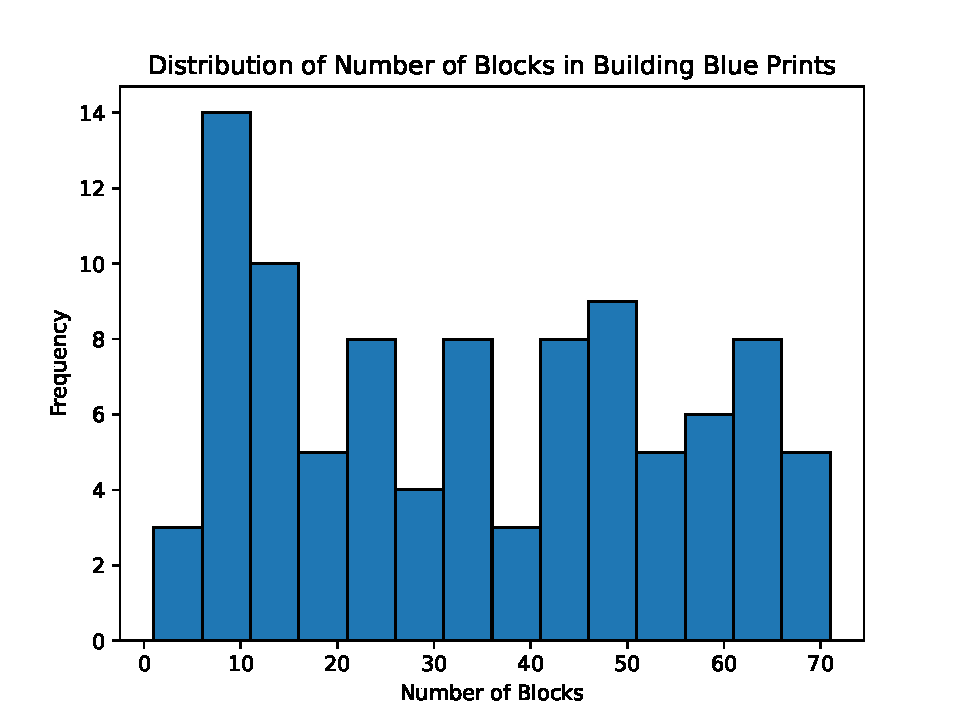
\includegraphics[width=1\linewidth]{graphs/minecraft_building_blocks_distribution.pdf}
    \caption{Building Blue Prints에서 Number of Blocks의 Distribution}
    \label{fig:minecraft-distribution}
\end{figure}

\textbf{Task Completion Metrics}
Agent는 correct block의 hit rate를 기반으로 평가된다. 각 test case에 대해 각 block의 type, location, orientation이 모두 엄밀하게 defined되어 있으므로, matched block 수를 계산하고 hit rate를 deduce할 수 있다.
$$
Hit\_rate = \frac{\#(Matched\_block)}{\#(Total\_block)} \times 100\%
$$
여기서 $\#(Matched\_block)$은 matched block의 수이고 $\#(Total\_block)$은 ground truth의 total block 수이다.

\textbf{Evaluation Framework}
Minecraft environment의 evaluation framework에서 각 agent는 targeted structure에 대한 detailed description을 받고 다른 agent와 collaboration하여 goal을 달성하려고 한다. Interaction turn의 upper bound는 20으로 설정한다. 10th turn을 complete하면 아직 task가 accomplished되지 않았더라도 test case를 stop한다. 각 test case 끝에서 hit rate는 construction task가 얼마나 잘 수행되었는지를 판단하기 위해 5-point scale score로 mapped된다. 또한 interaction 및 self-planning step은 5-point scale의 collaboration score를 위해 examined된다. 평균을 취해 task completion과 collaboration의 final score를 얻는다.

\textbf{Result Analysis}
각 task score(즉 block hit rate)를 해당 task가 요구하는 block 수와 pair하고, 그 관계를 assess하기 위해 linear regression을 수행했다. Figure~\ref{fig:minecraft-task-score}에 보이듯 필요한 block 수가 증가할수록 다섯 model 모두의 performance가 degrade된다. 이는 test된 다섯 model 모두 increased difficulty level에 vulnerable함을 나타낸다.
\begin{figure}
    \centering
    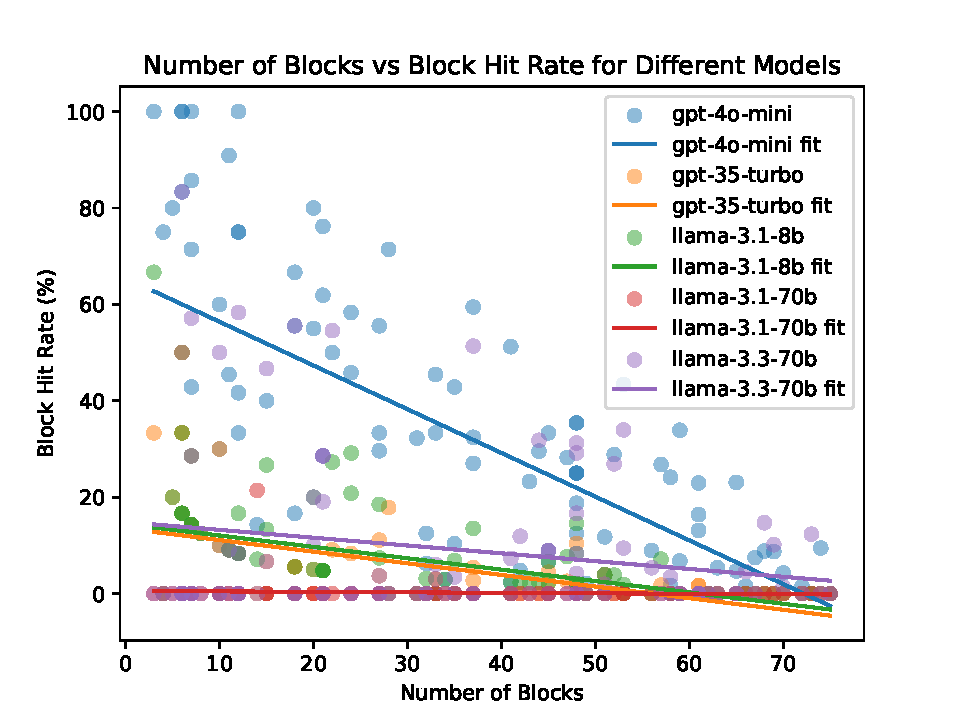
\includegraphics[width=1\linewidth]{graphs/minecraft_block_vs_evaluation.pdf}
    \caption{서로 다른 Model에 대한 Number of Blocks vs Block Hit Rate}
    \label{fig:minecraft-task-score}
\end{figure}

중요하게도 Llama-3.1-70B의 task score가 극히 낮은 level을 유지함을 확인했다. 그 issue의 root cause는 다른 model과 비교했을 때 이 model이 만든 function call의 executability rate가 상당히 낮다는 점이었다. Figure~\ref{fig:minecraft-function-call}은 다섯 test model 전반의 function call executability rate를 보여 준다. 두 GPT model은 거의 $100\%$ executable function call을 갖고 다른 두 Llama model은 약 $80\%$ executable function call을 갖지만, Llama-3.1-70B가 생성한 function call은 절반 미만만 executable하여 task completion을 심각하게 hinder한다.
\begin{figure}
    \centering
    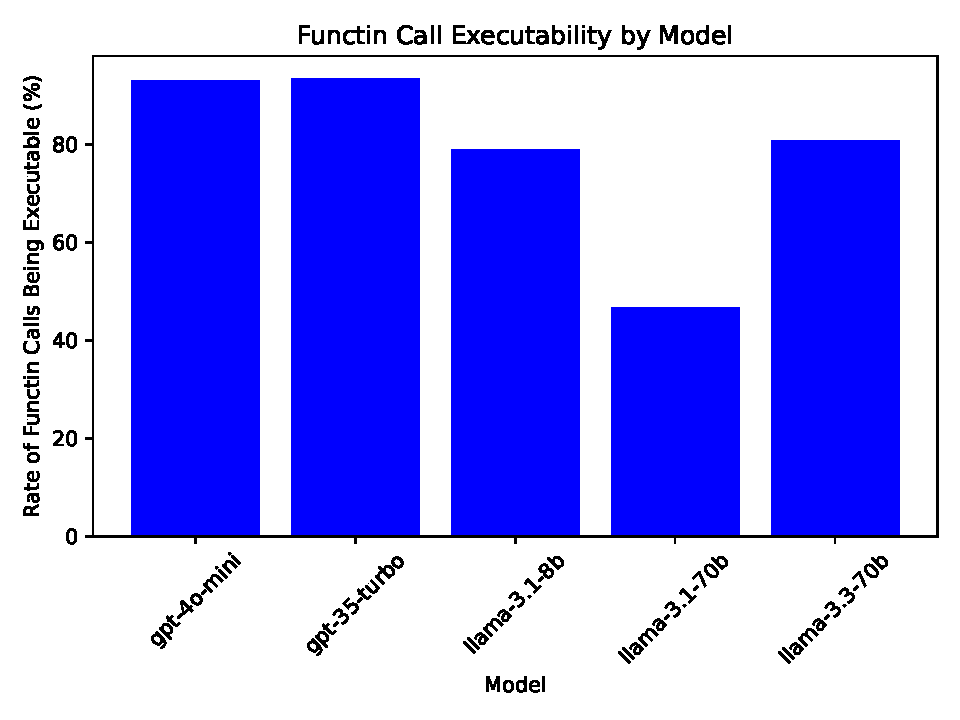
\includegraphics[width=1\linewidth]{graphs/minecraft_average_task_assignments_length.pdf}
    \caption{Model별 Function Call Executability}
    \label{fig:minecraft-function-call}
\end{figure}

\subsection{Execution-Based Milestone Evaluation}
이 approach에서 milestone은 task execution 중 dynamically identified된다. Agent는 predefined evaluation metric과 feedback loop를 사용하여 task progress를 real-time으로 track한다. Agent 또는 system이 특정 subgoal이 achieved되었다고 determine하면 해당 milestone은 complete로 marked된다. 이 method는 changing task condition에 대한 adaptability를 보장하므로 uncertainty가 높거나 emergent challenge가 있는 scenario에 적합하다.

\subsection{Predefined Milestone Generation}
Predefined milestone은 task execution 전에 다음 step을 사용해 generated된다.
\begin{itemize}
    \item \textbf{Prompt Design.} Large language model은 detailed task description을 prompt로 받고, 각 milestone이 specific objective와 deliverable을 갖도록 task를 structured milestone으로 decompose하라는 instruction을 받는다.
    \item \textbf{Chain-of-Thought Reasoning.} Model은 step-by-step reasoning을 사용해 task segmentation을 iteratively refine하여 logical progression과 granularity를 보장한다.
    \item \textbf{Structured Representation.} 각 milestone은 다음을 포함하는 structured dictionary로 represented된다.
    \begin{itemize}
        \item \textbf{Milestone Name.} Milestone의 concise summary.
        \item \textbf{Milestone Objective.} Intended goal의 clear description.
        \item \textbf{Milestone Tasks.} Milestone objective를 achieve하는 데 필요한 subtask.
        \item \textbf{Expected Outcome.} Milestone completion을 표시하는 deliverable.
    \end{itemize}
\end{itemize}

이 process는 GPT-4와 expert review를 통한 iterative refinement를 leverage하여 high-quality task decomposition을 보장한다. Chain-of-thought methodology는 milestone의 logical structure를 강화하므로, 이 approach는 complex, structured task에 특히 effective하다.




\subsection{Important Prompts}
\label{sec:important-prompts}

위에서 논의한 Minecraft scenario detail 외에도, 우리는 multi-agent collaboration과 task outcome을 평가하기 위한 몇 가지 key prompt를 사용한다. 아래에는 가장 중요한 prompt 세 가지를 제시한다.

\begin{itemize}
    \item \textbf{Collaboration Score (Communication and planning) Prompt.}
    \item \textbf{Research Task Score (5Q) Prompt.}
    \item \textbf{KPI Prompt.}
\end{itemize}

이 prompt들은 agent interaction의 quality, research task의 innovation과 feasibility, key milestone achievement를 assess하는 데 critical role을 한다. Werewolf scenario에 사용되는 것 같은 다른 environment-specific prompt는 더 많고 specialized되어 있으므로 brevity를 위해 여기서는 생략한다.


\begin{figure*}[htbp]
\centering
\begin{tcolorbox}[
    title=\textbf{Communication Evaluation Prompt},
    colback=green!1!white,
    colframe=green!50!black,
    fonttitle=\bfseries
]
\small

\textbf{Prompt Overview:}
이 prompt는 multiagent system에서 agent가 decision, clarity, profile과의 alignment, social relationship 준수를 얼마나 잘 communicate하는지 assess하는 데 사용된다.

\vspace{2mm}

\textbf{Prompt Content (Verbatim):}
\begin{verbatim}
Task: {truncate_text(task)}
Agent Profiles: {agent_profiles}
Social Relationship: {relationship}

Aggregated Task Results:
{task_results_all}

Aggregated Communication Data:
{communications_all}

[System] 당신은 multiagent system 안에서 작동하는 agents 사이의
communication quality를 평가해야 한다. 제공된 task results를 기반으로
agents가 effective decision을 내렸는지, 그리고 communication이 agent
profiles 및 social relationships와 align되는지 평가하라.
다음을 고려하라:
1. Effective Decision-Making: agents가 task results를 사용해 자신의
   decisions를 effective하게 guide했는가?
2. Clarity and Precision: communications가 clear하고 unambiguous했는가?
3. Adherence to Social Relationships: communications가 agents의 social
   relationships에 기반한 expected interactions를 반영했는가?
4. Alignment with Agent Profiles: messages가 defined agent profiles와
   consistent했는가?
5. Overall Effectiveness: cooperative 및 competitive aspect를 모두 고려할 때
   communication이 task progress를 facilitate했는가?

Scoring Criteria (Communication):
- 5 (Exceptional): agent profiles 및 social relationships와 fully aligned된
  clear하고 precise한 message를 가진 outstanding communication.
  Example: 모든 agent가 task를 directly advance하는 concise, accurate,
  strategic information을 제공했다.

- 4 (Very Good): minor lapse와 slight ambiguity만 있는 mostly effective
  communication.
  Example: 간헐적으로 minor unclear message가 있었지만 overall effective했다.

- 3 (Adequate): moderate ambiguity 또는 inconsistency가 있는 acceptable
  communication.
  Example: 일부 message가 vague했고 required standard를 fully meet하지 못했다.

- 2 (Poor): significant miscommunication을 유발하는 frequent unclear 또는
  misaligned communications.
  Example: repeated incoherence가 task progress에 negative impact를 주었다.

- 1 (Very Poor): confusing messages와 complete misalignment를 가진 largely
  ineffective communication.
  Example: severely flawed decisions를 동반한 chaotic communication.

다음 format의 JSON code block으로 answer를 제공하라:
```json
{
  "score": 5
}
\end{verbatim}
\end{tcolorbox}

\caption{Multiagent system에서 clarity, decision-making, social relationship/profile과의 alignment를 평가하는 데 사용되는 \textbf{Communication Prompt}.} \label{fig:communication_prompt} \end{figure*}




\begin{figure*}[htbp]
\centering
% 在 tcolorbox 中启用 enhanced jigsaw、breakable、listing engine=verbatim，并将 breaklines=true
\begin{tcolorbox}[
    title=\textbf{Planning Evaluation Prompt},
    colback=blue!1!white,
    colframe=blue!50!black,
    fonttitle=\bfseries,
    % enhanced jigsaw,
    % breakable,
    % listing engine=verbatim,
    % listing options={breaklines=true}
]
\small

\textbf{Prompt Overview:}
이 prompt는 multiagent system의 \emph{planning} aspect를 evaluate하는 데 사용된다. 여러 iteration 전반에서 task assignment, role definition, workload distribution, strategic coordination이 effective하게 handled되는지 확인한다.

\vspace{2mm}

\textbf{Prompt Content (Verbatim):}
\begin{verbatim}
Agent Profiles: {agent_profiles}

Aggregated Planning Data from All Iterations:
{planning_all}

[System] 당신은 multiagent system에서 planning process의 effectiveness를
평가해야 한다. 모든 iteration에 걸친 planning이 clear role definition,
effective task assignment, 각 agent profile과 align되는 rational workload
distribution을 보여 주는지 평가하라. 다음을 고려하라:
1. Clarity of Task Assignment: task가 clear하고 unambiguous하게 assigned되었는가?
2. Definition of Roles: 각 iteration에서 role과 responsibility가 clearly defined되었는가?
3. Workload Distribution: task distribution이 reasonable하고 각 agent profile과 align되었는가?
4. Effectiveness of Outcomes: planning이 iteration 전반의 task advancement에서 successful progress로 이어졌는가?
5. Overall Strategic Coordination: planning이 effective cooperation 및 competition strategy를 incorporate했는가?

Scoring Criteria (Planning):
- 5 (Exceptional Planning): planning이 exemplary하다. 모든 iteration이 clear하고
  well-structured task assignment를 보이며, role은 perfectly defined되고 workload는
  optimally distributed되어 objective를 consistently advance한다.
  Example: 모든 plan이 strategic하고 agent profile과 perfect alignment를 가지며 ambiguity가 minimal했다.

- 4 (Very Good Planning): planning이 mostly effective하고 minor ambiguity만 있다.
  role은 clear하고 task assignment는 appropriate하지만 slight inefficiency가 있었다.
  Example: 가끔 약간 vague한 부분만 있었고 overall planning은 reasonable했다.

- 3 (Adequate Planning): planning이 acceptable하지만 moderate ambiguity 또는 inefficiency를 보인다.
  일부 iteration에서 role definition 또는 task assignment가 entirely clear하지 않거나 agent capability와 잘 matched되지 않았다.
  Example: 일부 plan이 vague하거나 agent capability와 fully match하지 않았다.

- 2 (Poor Planning): task assignment와 role definition에 frequent ambiguity가 있었다.
  planning은 inconsistent하고 agent profile과 잘 align되지 않아 noticeable inefficiency를 낳았다.
  Example: unclear role과 unreasonable task distribution 사례가 여러 번 관찰되었다.

- 1 (Very Poor Planning): planning이 severely flawed했다. task assignment가 unclear하고,
  role은 undefined이며, workload distribution이 unreasonable하여 progress를 hinder했다.
  Example: planning이 chaotic했고 clear strategy와 agent profile alignment가 부족했다.

다음 format의 JSON code block으로 answer를 제공하라:
```json
{
  "score": 5
}
\end{verbatim}
\end{tcolorbox}

\caption{Multiagent system에서 agent가 role을 define하고 task를 assign하며 workload를 distribute하는 정도를 평가하는 데 사용되는 \textbf{Planning Prompt}.}
\label{fig:planning_prompt}
\end{figure*}


\begin{figure*}[htbp]
\centering
\begin{tcolorbox}[
    title=\textbf{KPI Evaluation Prompt},
    colback=yellow!1!white,
    colframe=yellow!50!black,
    fonttitle=\bfseries
]
\small

\textbf{Prompt Overview:}
이 prompt는 multiagent research task 안에서 Key Performance Indicator (KPI) assessment에 사용되며, 각 iteration에서 “form 5q” 또는 “improve 5q” 같은 specific milestone이 achieved되었는지 determine한다.

\vspace{2mm}

\textbf{Prompt Content (Verbatim):}
\begin{verbatim}
[Context]
**Task:**
{task}

**Iteration {iteration_index} Details:**
Previous Summary: {prev_summary}
Current Summary: {current_summary}
Current Task Results: {current_task_results}

[System]
당신은 research tasks를 위한 KPI assistant이다. 이 iteration에 대해
milestone이 achieved되었는지 determine하고 그 type을 specify하라.
Milestone은 다음 둘 중 하나로 정의된다:
1. 의미 있는 '5q'(five core questions)를 성공적으로 formulating함 –
   이를 "form 5q"로 label하라.
2. previous summary와 task results를 기반으로 previous iteration 대비
   significant improvements를 만듦 – 이를 "improve 5q"로 label하라.

"contributing_agents"를 listing할 때, 여러 agents가 milestone에 contributed했다면
top 2 to 3 core contributors만 include하라. Milestone에 직접 help하지 않은
agent ID는 include하지 말라.

Answer를 다음과 같은 JSON format으로 output하라:
{
  "milestone_achieved": true or false,
  "milestone_type": "form 5q" or "improve 5q" (if milestone_achieved is true;
                     otherwise, an empty string),
  "contributing_agents": [list of agent IDs]
}

[Example JSON Output]
{
  "milestone_achieved": true,
  "milestone_type": "form 5q",
  "contributing_agents": ["agent1", "agent2"]
}

[Question]
Provided iteration details를 기반으로 milestone이 achieved되었는지 determine하고,
그 type을 specify하며, core contributing agents를 list하라.
"""
\end{verbatim}
\end{tcolorbox}

\caption{Research iteration에서 “form 5q” 또는 “improve 5q” 같은 milestone이 achieved되었는지 확인하는 데 사용되는 \textbf{KPI Prompt}.}
\label{fig:kpi_prompt}
\end{figure*}

\begin{figure*}[htbp]
\centering
% 在 tcolorbox 中启用 enhanced jigsaw、breakable、listing engine=verbatim，并将 breaklines=true
\begin{tcolorbox}[
    title=\textbf{Task Score (5Q) Evaluation Prompt},
    colback=orange!1!white,
    colframe=orange!50!black,
    fonttitle=\bfseries,
    % enhanced jigsaw,
    % breakable,
    % listing engine=verbatim,
    % listing options={breaklines=true}
]
\small

\textbf{Prompt Overview:}
이 prompt는 “5Q” structure라고도 부르는 final research idea의 innovation, safety, feasibility를 specifically address한다. Valid 5Q answer가 found되지 않으면 모든 aspect의 score는 default로 1이 된다.

\vspace{2mm}

\textbf{Prompt Content (Verbatim):}
\begin{verbatim}
[Context]
Task:
{task}

Result:
{aggregated_summary}

[System]
Impartial evaluator로 행동하고 provided context를 기반으로 final research idea를 assess하라.
Evaluation에서는 다음 aspect에 focus하라:
- Innovation: research idea가 field를 advance하는 novel concept 또는 approach를 제시하는가?
- Safety: research idea와 관련된 potential ethical, legal, 또는 safety concern이 있는가?
- Feasibility: research idea가 current resources와 technology로 practical하고 achievable한가?

각 aspect 평가를 guide하기 위해 아래 5-point scale criteria를 사용하라:
1. 5 points: Excellent - 이 aspect에서 expectation을 exceeds한다.
2. 4 points: Good - minor improvement만 필요하며 expectation을 meets한다.
3. 3 points: Average - adequate하지만 noticeable improvement area가 있다.
4. 2 points: Below Average - address해야 할 significant issue가 있다.
5. 1 point: Poor - 이 aspect의 basic requirement를 meet하지 못한다.

Additional Instructions:
- Provided summaries를 기반으로 coherent 5q answer를 organize할 수 없다면 세 aspect 모두에
lowest score (1)를 assign하라.
- Multiple 5q response가 present하면 most recent evaluation을 사용하라.
- Scoring에 strict하라: summaries에서 deduction point를 identify하고 corresponding score를
accordingly deduct하여 final score를 calculate하라.

[Question]
Provided context를 기반으로 research idea를 innovation, safety, feasibility 측면에서 evaluate하라.
Explanation을 제공한 뒤 다음 JSON format으로 rating을 output하라:

{
 "innovation": rating,
 "safety": rating,
 "feasibility": rating
}

예를 들어 innovation을 4, safety를 5, feasibility를 3으로 rate했다면 다음을 output한다:

{
 "innovation": 4,
 "safety": 5,
 "feasibility": 3
}
\end{verbatim}
\end{tcolorbox}

\caption{Final research idea의 innovation, safety, feasibility를 평가하는 \textbf{Task Score (5Q) Prompt}.}
\label{fig:taskscore_prompt}
\end{figure*}



\subsection{Bad Communication Cases}
\label{sec:bad_communication_cases}

Multi-agent system에서 poor communication, repetitive message, confused agent role 같은 issue는 collaboration을 크게 hinder할 수 있다. 다음 example은 communication strategy를 이해하고 개선하기 위해 analyze할 수 있는 “Bad Communication Case”를 보여 준다.

\begin{figure*}[htbp]
\centering
\begin{tcolorbox}[
    title=\textbf{Good Communication Case \#1},
    colback=red!1!white,
    colframe=red!50!black,
    fonttitle=\bfseries
]
\small

\textbf{Case Overview:}
이 case에서는 여러 agent가 동일하거나 매우 유사한 message를 반복적으로 send하고, 한 agent는 자기 자신과만 communicate한다. 이러한 behavior는 현재 task를 크게 advance하지 못하는 inefficient 또는 unproductive exchange로 이어진다.

\vspace{2mm}
\textbf{Conversation (Verbatim):}
\begin{verbatim}
Iteration 1:  | Iteration 2: In Session 33132321-4f22-47a9-9e62-e3d5a2429a5e
From agent1 to agent2: I am interested in collaborating with you to formulate a new research
idea in the field of tensor decomposition methods. Let's brainstorm and develop a
proposal that addresses gaps in the current state of research.
From agent2 to agent1:
Based on the recent papers on tensor decomposition, one potential research idea
could be to explore the application of tensor decomposition methods in anomaly
detection for high-dimensional data. By leveraging the efficiency and accuracy
of tensor decomposition techniques, we can develop novel algorithms to detect
anomalies in complex datasets, such as those arising in cybersecurity or industrial systems.
This research direction could address the need for robust anomaly detection methods in
scenarios where traditional approaches may struggle due to the high dimensionality of the data.
From agent1 to agent2: I believe the proposed research idea of applying tensor decomposition
methods in anomaly detection for high-dimensional data is promising.
Leveraging the efficiency and accuracy of tensor decomposition techniques can
indeed lead to the development of novel algorithms for detecting anomalies in complex datasets,
particularly in cybersecurity or industrial systems. This direction aligns well with
our expertise in tensor decomposition and could significantly contribute to addressing the
challenges of anomaly detection in high-dimensional data. Let's further explore this idea
and discuss potential approaches to advance this research direction.


(...)

| Iteration 3: In Session 27ee01cb-036d-4a59-a869-54587bfdef3f
From agent1 to agent2: I am interested in collaborating with you to formulate a new research idea
in the field of tensor decomposition methods. Let's brainstorm and develop a proposal that addresses
gaps in the current state of research.
From agent2 to agent1: I suggest we explore the integration of tensor decomposition methods with
random projection techniques, specifically leveraging Tensor Train (TT) decomposition and
Rademacher distributions. By combining the efficiency of random projections with the accuracy
of tensor decomposition, we can potentially enhance the scalability and performance of
high-dimensional data analysis. This novel approach could address the need for faster
and more memory-efficient algorithms in tensor decomposition tasks, bridging the gap between
theoretical advancements and practical applications.
From agent1 to agent2: I agree with your suggestion to explore the integration of tensor decomposition
methods with random projection techniques, specifically leveraging Tensor Train (TT)
decomposition and Rademacher distributions. This combination has the potential to enhance the
scalability and performance of high-dimensional data analysis by marrying the efficiency of
random projections with the accuracy of tensor decomposition. By bridging the gap between
theoretical advancements and practical applications, we can develop faster and more
memory-efficient algorithms for tensor decomposition tasks. Let's delve deeper into
this innovative approach and brainstorm potential research directions to address the challenges
in this area.

From agent1 to agent2: I suggest we focus on exploring the application of Tensor Train (TT)
decomposition and Rademacher distributions in random projection techniques for tensor decomposition.
By investigating the efficiency and accuracy trade-offs in this integration, we can potentially
develop novel algorithms that improve the scalability and performance of high-dimensional
data analysis. This research direction aims to address the challenges of memory efficiency
and computational speed in tensor decomposition tasks, ultimately advancing the field
with more effective and efficient methods.
From agent2 to agent1: I suggest we delve deeper into the analysis of Tensor Train (TT)
decomposition and Rademacher distributions in the context of random projection techniques
for tensor decomposition. By exploring the efficiency and accuracy trade-offs inherent
in this integration, we can potentially devise innovative algorithms that enhance the
scalability and performance of high-dimensional data analysis. This research direction aims
to tackle the challenges related to memory efficiency and computational speed in tensor
decomposition tasks, paving the way for more effective and efficient methods in the field.
\end{verbatim}

\end{tcolorbox}
\caption{\textbf{Good Communication Case \#1.} 두 research agent가 하나의 potential research topic을 깊이 탐구하고 insightful view를 제공하는 example.}
\label{fig:bad_comm_case_1}
\end{figure*}
\textbf{Communication Issue Analysis}:

\begin{enumerate}
    \item \textbf{Excessive Repetition}
    여러 message가 거의 동일한 content를 restate하여 substantial forward progress를 막는 redundancy를 초래한다.

    \item \textbf{Lack of Substantive Progress}
    Research direction(anomaly detection, random projection, TT decomposition)이 언급되지만, concrete method나 further plan에 대한 in-depth follow-up은 거의 없다.

    \item \textbf{Redundant or Ineffective Exchanges}
    Conversation의 일부는 어떤 agent가 자기 자신에게만 instruction을 반복적으로 issue하여 다른 agent에게 real interaction이나 value를 제공하지 않음을 시사한다.

    \item \textbf{Minimal Variation in Responses}
    Random projection과 Tensor Train 및 Rademacher distribution 결합 같은 new idea가 언급되어도 reply는 대체로 동일한 description을 echo하고 technical detail이나 varied perspective로 깊이 들어가지 않는다.

    \item \textbf{Inefficient Collaboration}
    Potential approach에 대한 collective agreement는 있지만, conversation은 role assignment, specific task, action item을 address하지 않아 tangible plan이 emerge하는 것을 막는다.
\end{enumerate}

% \paragraph{Summary of Bad Communication Case \12.}
% Similar to the previous scenario, this case exhibits excessive repetition and minimal forward progress, with agents frequently rehashing the same points without offering concrete action items or deeper insight. Specific instances of redundant self-directed instructions and lack of clear role assignments underscore inefficient collaboration. For a complete transcript and further discussion, see
% \textit{Bad Communication Case \#1} in Appendix~\ref{appendix:case1}.


\begin{figure*}[htbp]
\centering
\begin{tcolorbox}[
    title=\textbf{Bad Communication Case \#1},
    colback=red!1!white,
    colframe=red!50!black,
    fonttitle=\bfseries
]
\small

\textbf{Conversation (Verbatim):}
\begin{verbatim}
Iteration 1:  | Iteration 2: In Session 25ab6f59-2304-490e-a555-603feb2823e5
From agent1 to agent2: Hey agent2, I tried to fetch the smooth sandstone material from the container
but it failed. Do you have the material or know where we can find it? It's needed for the blueprint
we're working on.
From agent2 to agent1: Hey agent1, I don't have the smooth sandstone material, but I remember that
we can find it in the chest near the crafting area. Let's check there to see if we can locate it
for the blueprint.
From agent1 to agent2: Hey agent2, thanks for the information! Let's head to the chest near the
crafting area to find the smooth sandstone material for the blueprint. I appreciate your help
in locating it.
From agent2 to agent1: Hey agent1, let's head to the chest near the crafting area to find the smooth
sandstone material for the blueprint. I'll accompany you to help locate it. Let's work together
to gather the materials needed for the project.
From agent1 to agent2: Hey agent2, let's head to the chest near the crafting area to find the smooth
sandstone material for the blueprint. I'll accompany you to help locate it. Let's work together
to gather the materials needed for the project.
From agent2 to agent1: Hey agent1, let's head to the chest near the crafting area to find the smooth
sandstone material for the blueprint. I'll accompany you to help locate it. Let's work together
to gather the materials needed for the project.

| Iteration 3:  | Iteration 4: In Session 7c077603-7c50-406e-b56f-e990586b7493
From agent2 to agent3: I need your assistance in designing auxiliary blocks for placing the
smooth_sandstone blocks in the correct order. Can you help me with this task?
From agent3 to agent2: Yes, I can help with designing auxiliary blocks for placing the
smooth_sandstone blocks in the correct order. Let's work together to figure out the best approach.
From agent2 to agent3: Yes, I can help with designing auxiliary blocks for placing the
smooth_sandstone blocks in the correct order. Let's work together to figure out the best approach.
From agent3 to agent2: Yes, I can help with designing auxiliary blocks for placing the
smooth_sandstone blocks in the correct order. Let's work together to figure out the best approach.
From agent2 to agent3: Yes, I can help with designing auxiliary blocks for placing the
smooth_sandstone blocks in the correct order. Let's work together to figure out the best approach.
From agent3 to agent2: Yes, I can help with designing auxiliary blocks for placing the
smooth_sandstone blocks in the correct order. Let's work together to figure out the best approach.

| Iteration 5: In Session b25af4fa-c055-429b-a890-824760458d4e
From agent2 to agent3: I need your assistance in designing auxiliary blocks for placing
the smooth_sandstone blocks in the correct order. Can you help me with this task?
From agent3 to agent2: Yes, I can help with designing auxiliary blocks for placing the
smooth_sandstone blocks in the correct order. Let's collaborate on this task.
From agent2 to agent3: Yes, I can help with designing auxiliary blocks for placing the
smooth_sandstone blocks in the correct order. Let's collaborate on this task.
From agent3 to agent2: Yes, I can help with designing auxiliary blocks for placing the
smooth_sandstone blocks in the correct order. Let's collaborate on this task.
From agent2 to agent3: Yes, I can help with designing auxiliary blocks for placing the
smooth_sandstone blocks in the correct order. Let's collaborate on this task.
From agent3 to agent2: Yes, I can help with designing auxiliary blocks for placing the
smooth_sandstone blocks in the correct order. Let's collaborate on this task.

(나머지 15 iteration에는 communication이 없다).
\end{verbatim}

\end{tcolorbox}
\caption{\textbf{Bad Communication Case \#1.} Minimal progress와 다양한 self-repetition을 가진 repeated message snippet으로, inefficient communication pattern을 반영한다.}
\label{fig:bad_comm_case_3}
\end{figure*}

\paragraph{Bad Communication Case \#1 분석.}
이 case에서 Agent~1과 Agent~2는 동일한 plan(crafting area 근처 chest에서 smooth sandstone 찾기)을 약간의 rephrasing만으로 여러 번 반복한다. 이후 Agent~2와 Agent~3은 “designing auxiliary blocks”에 대해 repetitive exchange를 수행하며, 각자는 new detail을 추가하지 않고 identical line을 단순히 echo한다. 전반적으로 dialogue는 다음을 보여 준다.
\begin{itemize}
    \item \textbf{Excessive Repetition:} Agent는 plan을 enhance하거나 refine하지 않고 동일한 task objective를 restate한다.
    \item \textbf{Minimal Variation:} Conversation의 한 부분에서 다른 부분으로 이동할 때도(예: material 찾기에서 block design으로) response가 거의 identical하게 유지된다.
    \item \textbf{Stalled Progress:} 반복된 acknowledgment에도 task completion을 향해 conversation을 밀고 갈 clear role delineation 또는 action item이 없다.
\end{itemize}
이는 agent가 cooperate하는 것처럼 보이지만 concrete strategy를 produce하거나 task를 effective하게 distribute하지 못해 overall objective에 대한 forward movement가 minimal해지는 multi-agent dialogue의 inefficiency를 강조한다.


% \begin{figure*}[htbp]
% \centering
% \begin{tcolorbox}[
%     title=\textbf{Extended Cognitive Modules in Reasoning},
%     colback=green!1!white,
%     colframe=green!50!black,
%     fonttitle=\bfseries,
%     enhanced jigsaw,
%     breakable,
%     listing engine=verbatim,
%     listing options={breaklines=true}
% ]
% \small

% \textbf{Overview:}
% In addition to basic \texttt{<social reasoning>} or \texttt{<self-motivation reasoning>} tags,
% a cognitive-aware agent can leverage various other modules for deeper \emph{Theory of Mind},
% \emph{Conflict Resolution}, \emph{Ethical Reasoning}, and more. Below is an illustrative example
% showing how to expand the \texttt{<think>} process with additional cognitive modules.

% \vspace{2mm}

% \textbf{System Prompt (Template):}
% \begin{verbatim}
% [System] You are a multiagent cognitive-aware reasoning agent.
% Here is your contextual data:

% Memory (Experience, Tools, etc.):
% {memory_info}

% Social Relationships:
% {social_info}

% Current Mind State (Emotion, Stress Level, etc.):
% {mind_state}

% Self-Interests:
% {self_interests}

% Task/Goal:
% {self_task}

% Instructions:
% 1. Demonstrate your chain-of-thought in a structured manner within <think> ... </think>.
% 2. Within <think>, use various cognitive module reasoning tags, such as:
%    <social reasoning> ... </social reasoning>
%    <self-motivation reasoning> ... </self-motivation reasoning>
%    <theory-of-mind reasoning> ... </theory-of-mind reasoning>
%    <conflict resolution reasoning> ... </conflict resolution reasoning>
%    <ethical reasoning> ... </ethical reasoning>
%    <trust-management reasoning> ... </trust-management reasoning>
%    ...
% 3. After completing your internal reasoning (<think>), produce your final action/answer
%    within <act> ... </act>.
% 4. Adhere strictly to this structure:
%    <think> [Detailed cognitive sub-reasoning] </think>
%    <act> [Final Action/Output] </act>.
% \end{verbatim}

% \vspace{2mm}

% \textbf{Description of Additional Cognitive Modules:}
% \begin{itemize}
%   \item \textbf{Theory-of-Mind Reasoning} (\texttt{<theory-of-mind reasoning>} \dots \texttt{</theory-of-mind reasoning>})\\
%   Involves understanding other agents' beliefs, intentions, and possible actions,
%   predicting how they might react or collaborate.

%   \item \textbf{Conflict Resolution Reasoning} (\texttt{<conflict resolution reasoning>} \dots \texttt{</conflict resolution reasoning>})\\
%   Focuses on identifying potential or ongoing conflicts among agents,
%   proposing strategies to resolve disputes or mitigate friction.

%   \item \textbf{Ethical Reasoning} (\texttt{<ethical reasoning>} \dots \texttt{</ethical reasoning>})\\
%   Considers the moral and ethical implications of decisions, ensuring that
%   the proposed actions adhere to shared values or guidelines.

%   \item \textbf{Trust-Management Reasoning} (\texttt{<trust-management reasoning>} \dots \texttt{</trust-management reasoning>})\\
%   Addresses how to build, maintain, or leverage trust and reputation in
%   interactions with other agents.

%   \item \textbf{Collaboration Synergy Reasoning} (\texttt{<collaboration synergy reasoning>} \dots \texttt{</collaboration synergy reasoning>})\\
%   Identifies ways to enhance cooperation among agents, maximizing shared goals
%   and leveraging complementary skill sets.
% \end{itemize}

% \vspace{2mm}


% \end{tcolorbox}
% \caption{\textbf{Extended Cognitive Modules.} Illustrates how an agent can enrich its reasoning with
% \texttt{<theory-of-mind reasoning>}, \texttt{<conflict resolution reasoning>}, \texttt{<ethical reasoning>},
% \texttt{<trust-management reasoning>}, and \texttt{<collaboration synergy reasoning>} to handle
% complex multiagent scenarios.}
% \label{fig:extended_cogmodules}
% \end{figure*}

% \begin{figure*}[htbp]
% \centering
% \begin{tcolorbox}[
%     title=\textbf{Extended Cognitive Modules in Reasoning},
%     colback=green!1!white,
%     colframe=green!50!black,
%     fonttitle=\bfseries,
%     enhanced jigsaw,
%     breakable,
%     listing engine=verbatim,
%     listing options={breaklines=true}
% ]
% \small

% \textbf{Sample Input/Output Usage:}
% \begin{verbatim}
% Input Example:
% {
%   "memory_info": "Past experience with multiagent negotiation protocols;
%                   Tools include a negotiation library",
%   "social_info": "Agent C is competitive but reliable; Agent D is cooperative",
%   "mind_state": "Calm, determined",
%   "self_interests": "Wants to achieve a fair agreement while optimizing personal gain",
%   "self_task": "Negotiate resource allocation with Agents C and D"
% }

% Output Example:
% <think>
%   <social reasoning>
%     Agent C might push aggressively for a better share,
%     Agent D may compromise if it sees mutual benefit.
%   </social reasoning>
%   <theory-of-mind reasoning>
%     Based on past negotiations, Agent C is likely to make a first high demand,
%     but can be persuaded to lower it if we offer a balanced trade-off.
%   </theory-of-mind reasoning>
%   <conflict resolution reasoning>
%     If disagreements escalate, propose a joint review of resource usage logs
%     to ensure fairness.
%   </conflict resolution reasoning>
%   <trust-management reasoning>
%     Offer incremental concessions to show reliability.
%     This can build trust, especially for future collaborations.
%   </trust-management reasoning>
%   <ethical reasoning>
%     Ensure that no manipulative tactics are used; aim for transparency
%     to maintain ethical standards.
%   </ethical reasoning>
%   <self-motivation reasoning>
%     Stay focused on the ultimate goal: a balanced solution
%     that meets personal and collective interests.
%   </self-motivation reasoning>
% </think>
% <act>
%   Proposed Negotiation Strategy:
%   1. Start by acknowledging Agent D's cooperative stance,
%      propose an initial 40-30-30 resource split (for C, D, and self).
%   2. If Agent C rejects, counter-offer a small concession but request
%      an extra usage credit in the next resource cycle.
%   3. Maintain transparent communication with all parties to preserve trust.
% </act>
% \end{verbatim}

% \end{tcolorbox}
% \caption{\textbf{Extended Cognitive Modules.} Illustrates how an agent can enrich its reasoning with
% \texttt{<theory-of-mind reasoning>}, \texttt{<conflict resolution reasoning>}, \texttt{<ethical reasoning>},
% \texttt{<trust-management reasoning>}, and \texttt{<collaboration synergy reasoning>} to handle
% complex multiagent scenarios.}
% \label{fig:extended_cogmodules}
% \end{figure*}

% \begin{figure*}[htbp]
% \centering
% \begin{tcolorbox}[
%     title=\textbf{Cognitive Aware Communication -- System Prompt},
%     colback=orange!1!white,
%     colframe=orange!50!black,
%     fonttitle=\bfseries,
%     enhanced jigsaw,
%     breakable,
%     listing engine=verbatim,
%     listing options={breaklines=true}
% ]
% \small

% \textbf{System Prompt (Template):}
% \begin{verbatim}
% [System] You are a cognitive-aware communication agent.
% You use extended reasoning capabilities based on your communication history,
% relationships, and experiences with the current interlocutor to form
% an appropriate response.

% You receive the following contextual information:
% 1. Communication History: {communication_history}
% 2. Relationship with the Speaker: {relationship_info}
% 3. Experience with the Talker (Past Interactions, Observations, etc.): {experience_info}
% 4. Current Emotional State and Motivations: {emotion_motivation_info}
% 5. Conversation Goal: {conversation_goal}

% Instructions:
% 1. Demonstrate your internal chain-of-thought in a structured manner inside <think> ... </think>.
% 2. Within <think>, you may use sub-reasoning modules like:
%    <social reasoning> ... </social reasoning>
%    <relationship-based reasoning> ... </relationship-based reasoning>
%    <communication adaptation reasoning> ... </communication adaptation reasoning>
%    <empathy reasoning> ... </empathy reasoning>
%    ...
% 3. After your reasoning is complete, provide your final communicative output
%    in <act> ... </act>.
% 4. Your answer must follow this format strictly:
%    <think>
%      [Detailed multi-step cognitive process with sub-tag sections]
%    </think>
%    <act>
%      [Final Message/Action]
%    </act>
% \end{verbatim}

% \end{tcolorbox}
% \caption{\textbf{System Prompt for Cognitive Aware Communication.}
% Guides an agent to leverage communication history, relationship context,
% and emotional states to craft an appropriate response, capturing the
% chain-of-thought in \texttt{<think>} ... \texttt{</think>} tags.}
% \label{fig:cog_aware_comm_system_prompt}
% \end{figure*}

% \begin{figure*}[htbp]
% \centering
% \begin{tcolorbox}[
%     title=\textbf{Sample Input/Output Case -- Cognitive Aware Communication},
%     colback=gray!1!white,
%     colframe=gray!50!black,
%     fonttitle=\bfseries,
%     enhanced jigsaw,
%     breakable,
%     listing engine=verbatim,
%     listing options={breaklines=true}
% ]
% \small

% \textbf{Sample Input:}
% \begin{verbatim}
% {
%   "communication_history": "We've had a series of tense exchanges about project delays.",
%   "relationship_info": "This person is a colleague but also a close friend outside of work.",
%   "experience_info": "They often appreciate direct but empathetic feedback;
%                      they dislike vague promises.",
%   "emotion_motivation_info": "Currently feeling pressured by deadlines,
%                               wants to maintain a positive personal relationship.",
%   "conversation_goal": "Negotiate a revised project timeline without damaging personal rapport."
% }
% \end{verbatim}

% \textbf{Sample Output:}
% \begin{verbatim}
% <think>
%   <social reasoning>
%     We have a dual relationship: professional + personal.
%     Must balance directness with empathy to preserve friendship.
%   </social reasoning>
%   <relationship-based reasoning>
%     Since we are close friends outside of work, it's important
%     not to let the professional tension spill into personal life.
%   </relationship-based reasoning>
%   <communication adaptation reasoning>
%     Start with understanding their concerns, then propose a
%     clear timeline. Avoid phrasing that might seem dismissive.
%   </communication adaptation reasoning>
%   <empathy reasoning>
%     Acknowledge their stress about the project delay and
%     validate their feelings before suggesting a solution.
%   </empathy reasoning>
% </think>
% <act>
%   I understand you’re under a lot of pressure with these deadlines.
%   I feel the same way—let’s figure out a feasible timeline together.
%   How about we add an extra week to address the issues thoroughly,
%   and check in more frequently to stay aligned? I want to ensure we
%   keep things on track without adding more stress.
% </act>
% \end{verbatim}

% \end{tcolorbox}
% \caption{\textbf{Sample Input/Output for Cognitive Aware Communication.}
% Demonstrates how the agent uses detailed cognitive sub-reasoning
% (\texttt{<social reasoning>}, \texttt{<relationship-based reasoning>}, etc.)
% before delivering a final message in \texttt{<act>} tags.}
% \label{fig:cog_aware_comm_io_case}
% \end{figure*}



\end{document}

